
\documentclass[]{interact}
\usepackage{epstopdf}% To incorporate .eps illustrations using PDFLaTeX, etc.
\usepackage[caption=false]{subfig}% Support for small, `sub' figures and tables
\usepackage{array}% Support controlled alignment in paragraph-style table columns
\renewcommand{\thesubfigure}{\textit{\alph{subfigure}}}% IJRS style: italic subfigure letters in roman parentheses
\usepackage[section]{placeins}% Prevent figures and tables from drifting beyond their section
\setcounter{topnumber}{3}
\setcounter{bottomnumber}{2}
\setcounter{totalnumber}{5}
\renewcommand{\topfraction}{0.90}
\renewcommand{\bottomfraction}{0.80}
\renewcommand{\textfraction}{0.08}
\renewcommand{\floatpagefraction}{0.75}
\widowpenalty=10000
\clubpenalty=10000
\displaywidowpenalty=10000

\usepackage[natbibapa]{apacite}% APA author-year citation support. Commands using natbib.sty MUST be deactivated first!
\setlength\bibhang{12pt}% To set the indentation in the list of references using apacite.sty.
\renewcommand\bibliographytypesize{\fontsize{10}{11.8}\selectfont}% Keep 10-point references while avoiding an otherwise nearly empty final page.
\usepackage[colorlinks=true, citecolor=blue, linkcolor=blue, urlcolor=blue]{hyperref}% Clickable hyperlinks


\theoremstyle{plain}% Theorem-like structures provided by amsthm.sty
\newtheorem{theorem}{Theorem}[section]
\newtheorem{lemma}[theorem]{Lemma}
\newtheorem{corollary}[theorem]{Corollary}
\newtheorem{proposition}[theorem]{Proposition}

\theoremstyle{definition}
\newtheorem{definition}[theorem]{Definition}
\newtheorem{example}[theorem]{Example}

\theoremstyle{remark}
\newtheorem{remark}{Remark}
\newtheorem{notation}{Notation}

% Revision markup generated from the supplied original and current sources.
\usepackage[normalem]{ulem}
\usepackage{color}
\usepackage[left]{lineno}
\definecolor{DIFaddcolor}{RGB}{0,63,180}
\definecolor{DIFdelcolor}{RGB}{220,35,35}
\DeclareRobustCommand{\DIFadd}[1]{{\protect\color{DIFaddcolor}\uwave{#1}}}
\DeclareRobustCommand{\DIFdel}[1]{{\protect\color{DIFdelcolor}\sout{#1}}}
\widowpenalty=10000
\clubpenalty=10000
\displaywidowpenalty=10000
\pdfstringdefDisableCommands{%
  \def\DIFadd#1{#1}%
  \def\DIFdel#1{}%
}

\begin{document}
\linenumbers

\articletype{Review Article}% Specify the article type or omit as appropriate

\title{Deep learning and multi-level fusion for land-use and land-cover classification: Technological evolution trajectory and future trends}

\author{
\name{Jie Cheng\textsuperscript{a}, Jie Xie\textsuperscript{a}\thanks{CONTACT Jie Xie. Email: xiej8734@gmail.com}, Shupei Xia\textsuperscript{a} and Alejandro C.\ Frery\textsuperscript{b}}
\affil{\textsuperscript{a}School of Computer and Electronic Information / School of Artificial Intelligence, Nanjing Normal University, Nanjing, China; \textsuperscript{b}School of Mathematics and Statistics, Victoria University of Wellington, New Zealand}
}

\maketitle

\noindent\footnotesize\textit{Revision markup: deleted text is shown in red with strikeout, and added text is shown in blue with a wavy underline. The newly added fusion-level comparison table is shown in blue. Model-table edits are marked within individual cells; references are placed below the table for readability. In the bibliography, red entries are the original versions and blue entries are the revised or newly added versions.}\normalsize\par\medskip

\begin{abstract}
Land Use/Land Cover \DIFdel{Change} (\DIFdel{LULCC}\hspace{0.33em}\DIFadd{LULC}) \DIFadd{classification} is essential to understand human-environment interactions, ecological impacts, and sustainable land management. Given the growing complexity and scale of \DIFdel{LULCC} \DIFdel{dynamics} \DIFadd{Earth} \DIFadd{observation} \DIFadd{data}, accurately \DIFdel{capturing} \DIFdel{these} \DIFdel{processes} \DIFadd{classifying} \DIFadd{LULC} remains a significant challenge. With the development of Earth observation technology and artificial intelligence, deep learning combined with multi-source data fusion has \DIFdel{become} \DIFdel{the} \DIFdel{core} \DIFdel{driving} \DIFdel{force} \DIFadd{received} \DIFadd{increasing} \DIFadd{attention} for \DIFdel{the} \DIFdel{LULCC} \DIFdel{simulation} \DIFadd{LULC} \DIFadd{classification}. To clarify the trajectory of technological evolution and future trends in this field, this study conducts an in-depth analysis of 261 \DIFdel{core} \DIFdel{literatures} \DIFadd{publications} published from 2006 to 2025 based on the Web of Science Core Collection, integrating \DIFdel{systematic} \DIFadd{technical} and bibliometric review methods\DIFadd{.} \DIFadd{The} \DIFadd{search} \DIFadd{required} \DIFadd{both} \DIFadd{deep} \DIFadd{learning} \DIFadd{and} \DIFadd{fusion} \DIFadd{terms}\DIFadd{;} \DIFadd{it} \DIFadd{does} \DIFadd{not} \DIFadd{represent} \DIFadd{the} \DIFadd{entire} \DIFadd{LULC} \DIFadd{literature}. Our results show that: (1) The number of published papers in this \DIFdel{field} \DIFadd{corpus} has \DIFdel{witnessed} \DIFdel{an} \DIFdel{exponential} \DIFdel{growth} \DIFadd{increased} \DIFadd{substantially} since 2016; (2) \DIFdel{In} \DIFdel{terms} \DIFdel{of} \DIFdel{technological} \DIFdel{paradigms}\DIFdel{,} \DIFadd{Research} \DIFadd{attention} \DIFadd{within} the \DIFdel{research} \DIFdel{focus} \DIFdel{has} \DIFdel{undergone} \DIFdel{a} \DIFdel{fundamental} \DIFdel{shift} \DIFdel{from} \DIFdel{single} \DIFdel{data} \DIFdel{source} \DIFdel{and} \DIFdel{traditional} \DIFdel{machine} \DIFdel{learning} \DIFdel{to} \DIFadd{corpus} \DIFadd{centres} \DIFadd{on} multi-source heterogeneous data fusion and deep learning; (3) \DIFadd{The} \DIFadd{suitability} \DIFadd{of} \DIFadd{data-level}\DIFadd{,} feature-level \DIFdel{fusion} \DIFdel{has} \DIFdel{replaced} \DIFdel{data-level}\DIFadd{,} and decision-level fusion \DIFdel{as} \DIFdel{the} \DIFdel{current} \DIFdel{main} \DIFdel{strategy} \DIFadd{depends} \DIFadd{on} \DIFadd{data} \DIFadd{alignment}\DIFadd{,} \DIFadd{training} \DIFadd{resources}\DIFadd{,} \DIFadd{and} \DIFadd{application} \DIFadd{requirements}; (4) Future research should focus on the development of Explainable Artificial Intelligence, \DIFdel{general} remote sensing foundation models, \DIFadd{uncertainty-aware} \DIFadd{learning}\DIFadd{,} and \DIFdel{intelligent} \DIFadd{multimodal} data governance technologies.
\end{abstract}

\begin{keywords}
\DIFdel{Land} \DIFdel{Use}\DIFdel{/}\DIFdel{Land} \DIFdel{Cover}\DIFdel{,}
\DIFadd{Land-use} \DIFadd{and} \DIFadd{land-cover} \DIFadd{classification}\DIFadd{;} deep learning\DIFdel{,}\DIFadd{;} multi-source data fusion\DIFdel{,}\DIFadd{;} feature fusion\DIFdel{,}\DIFadd{;} Transformer\DIFdel{,}\DIFadd{;} Mamba
\end{keywords}


\section{Introduction}

Land-use and land-cover (LULC) information constitutes a fundamental baseline for understanding Earth system dynamics and is pivotal in urban planning, ecosystem assessment, disaster monitoring, and global climate change research {\hypersetup{citecolor=red}\color{red}\citep{ORIG1}} {\color{blue}\citep{1}}. However, optical remote sensing alone is insufficient to capture the full complexity of land surface processes. Consequently, complementary modalities including \DIFadd{light} \DIFadd{detection} \DIFadd{and} \DIFadd{ranging} \DIFadd{(}LiDAR\DIFdel{,}\DIFadd{)} \DIFadd{and} \DIFadd{synthetic} \DIFadd{aperture} \DIFadd{radar} \DIFadd{(}SAR\DIFdel{,} \DIFdel{and} \DIFdel{GNSS}\DIFadd{)} are increasingly \DIFdel{essential} \DIFadd{used}, as they provide \DIFdel{unique} structural\DIFdel{,} \DIFdel{temporal}\DIFdel{,} and \DIFdel{positional} \DIFadd{all-weather} information. With the rapid advancement of Earth observation technologies that integrate these multi-source data, the field has entered the era of remote sensing big data, \DIFdel{characterized} \DIFadd{characterised} by high spatial, temporal, and \DIFdel{hyperspectral} \DIFadd{spectral} resolutions. Nonetheless, accurate and automated classification of complex Earth \DIFdel{surface} \DIFdel{dynamics} \DIFadd{surfaces} remains a significant challenge in geographic information science.


Historically, LULC classification initially relied on statistical methods such as Gaussian maximum likelihood classification and later shifted to traditional machine learning algorithms like Support Vector Machines (SVM) and Random Forest (RF). While effective \DIFdel{for} \DIFdel{small-scale} \DIFdel{areas} \DIFadd{with} \DIFadd{suitable} \DIFadd{features} \DIFadd{and} \DIFadd{limited} \DIFadd{training} \DIFadd{samples}, these shallow models \DIFdel{often} \DIFdel{fail} \DIFdel{to} \DIFadd{may} \DIFadd{not} capture high-level semantic features and depend substantially on manual feature engineering, which \DIFdel{consequently} \DIFdel{limits} \DIFadd{can} \DIFadd{limit} their \DIFdel{generalization} \DIFadd{generalisation} capabilities in complex heterogeneous scenes. Since 2015, the emergence of Deep Learning (DL) has substantially transformed the field \citep{2}. Algorithms including Convolutional Neural \DIFdel{Network} \DIFadd{Networks} (\DIFdel{CNN}\hspace{0.33em}\DIFadd{CNNs}) and the more recent \DIFdel{Transformer} \DIFdel{have} \DIFdel{consistently} \DIFdel{outperformed} \DIFdel{traditional} \DIFdel{methods} \DIFdel{by} \DIFadd{Transformers} \DIFadd{can} automatically \DIFdel{learning} \DIFadd{learn} hierarchical representations directly from raw data\DIFadd{.} \DIFadd{Their} \DIFadd{performance} \DIFadd{relative} \DIFadd{to} \DIFadd{traditional} \DIFadd{methods} \DIFadd{depends} \DIFadd{on} \DIFadd{the} \DIFadd{dataset}\DIFadd{,} \DIFadd{training} \DIFadd{samples}\DIFadd{,} \DIFadd{sensor} \DIFadd{combination}\DIFadd{,} \DIFadd{and} \DIFadd{evaluation} \DIFadd{protocol}.


Parallel to the evolution of algorithms, the limitations of single-source remote sensing data have become increasingly prominent. Optical imagery is susceptible to cloud cover and lighting conditions, SAR lacks rich spectral information, and LiDAR data \DIFdel{is} \DIFadd{are} often constrained by acquisition costs. Consequently, multi-source data fusion that integrates the complementary strengths of optical imagery in terms of spectral content, SAR with respect to texture, structure, and dielectric properties, and LiDAR for elevation information has \DIFdel{become} \DIFdel{an} \DIFdel{inevitable} \DIFadd{been} \DIFadd{investigated} \DIFadd{as} \DIFadd{a} strategy to \DIFdel{overcome} \DIFdel{the} \DIFdel{accuracy} \DIFdel{limitations} \DIFdel{of} \DIFadd{improve} LULC classification. The intersection of deep learning and multi-source fusion \DIFdel{now} \DIFdel{represents} \DIFdel{the} \DIFdel{current} \DIFdel{technical} \DIFdel{frontier} \DIFadd{has} \DIFadd{attracted} \DIFadd{increasing} \DIFadd{research} \DIFadd{attention}. Despite the \DIFdel{exponential} growth in publications, a comprehensive understanding of how these technologies have evolved over the past two decades remains relatively fragmented \citep{5}\DIFadd{.}

\DIFadd{Sensor} \DIFadd{observations} \DIFadd{are} \DIFadd{not} \DIFadd{the} \DIFadd{only} \DIFadd{relevant} \DIFadd{information} \DIFadd{source}\DIFadd{.} \DIFadd{Crowdsourced} \DIFadd{geographic} \DIFadd{information} \DIFadd{can} \DIFadd{provide} \DIFadd{labels}\DIFadd{,} \DIFadd{semantic} \DIFadd{context}\DIFadd{,} \DIFadd{and} \DIFadd{rapid} \DIFadd{updates} \DIFadd{for} \DIFadd{LULC} \DIFadd{mapping}\DIFadd{,} \DIFadd{but} \DIFadd{its} \DIFadd{spatial} \DIFadd{coverage}\DIFadd{,} \DIFadd{positional} \DIFadd{accuracy}\DIFadd{,} \DIFadd{contributor} \DIFadd{bias}\DIFadd{,} \DIFadd{class} \DIFadd{consistency}\DIFadd{,} \DIFadd{and} \DIFadd{licensing} \DIFadd{conditions} \DIFadd{require} \DIFadd{explicit} \DIFadd{quality} \DIFadd{control} {\color{blue}\citep{wu2024crowdsourced}}\DIFadd{.} \DIFadd{In} \DIFadd{this} \DIFadd{review}\DIFadd{,} \emph{\DIFadd{multi-source} \DIFadd{fusion}} \DIFadd{denotes} \DIFadd{the} \DIFadd{integration} \DIFadd{of} \DIFadd{observations} \DIFadd{or} \DIFadd{derived} \DIFadd{products} \DIFadd{from} \DIFadd{multiple} \DIFadd{sources}\DIFadd{,} \DIFadd{whereas} \emph{\DIFadd{multimodal} \DIFadd{learning}} \DIFadd{denotes} \DIFadd{models} \DIFadd{that} \DIFadd{learn} \DIFadd{from} \DIFadd{data} \DIFadd{with} \DIFadd{different} \DIFadd{measurement} \DIFadd{or} \DIFadd{representational} \DIFadd{characteristics}\DIFadd{.} \DIFadd{These} \DIFadd{terms} \DIFadd{are} \DIFadd{therefore} \DIFadd{related} \DIFadd{but} \DIFadd{not} \DIFadd{interchangeable}.

Although numerous review articles on LULC classification or remote sensing data fusion have been published, existing studies face several limitations in meeting the demand for a macro-scale understanding of the field's evolution. First, existing reviews often focus on a single technical lineage and suffer from a time lag. For instance, Ma et al. systematically \DIFdel{summarized} \DIFadd{summarised} the early applications of deep learning in remote sensing, but their focus was primarily on CNN architectures {\hypersetup{citecolor=red}\color{red}\citep{ORIGma2019deep}} {\color{blue}\citep{56}}. Since their work predates the emergence of Vision \DIFdel{Foundation} \DIFdel{Models} \DIFdel{such} \DIFdel{as} \DIFdel{Transformer} \DIFadd{Transformers} and State Space Models like Mamba \DIFdel{after} \DIFdel{2020}, it fails to cover \DIFdel{the} \DIFdel{latest} \DIFdel{technical} \DIFdel{paradigm} \DIFdel{shifts} \DIFadd{these} \DIFadd{subsequent} \DIFadd{developments}. While recent scholars including Aleissaee et al. have provided \DIFdel{specialized} \DIFadd{specialised} reviews on Transformers, they concentrate on emerging technologies with limited discussion of previous traditional algorithms \citep{7}. Second, there is a lack of quantitative scientometric support. Although Ghamisi et al. provided a detailed technical \DIFdel{categorization} \DIFadd{categorisation} of multi-source data fusion strategies including data-level, feature-level, and decision-level fusion, their work remains a qualitative technical review {\hypersetup{citecolor=red}\color{red}\citep{ORIG6,7,8}} {\color{blue}\citep{6}}. \DIFdel{Such} \DIFdel{articles} \DIFdel{tend} \DIFdel{to} \DIFdel{list} \DIFdel{algorithmic} \DIFdel{details} \DIFdel{without} \DIFdel{the} \DIFdel{support} \DIFdel{of} \DIFdel{large-sample} Bibliometric analysis\DIFdel{,} \DIFdel{making} \DIFdel{it} \DIFdel{difficult} \DIFdel{for} \DIFdel{researchers} \DIFdel{to} \DIFdel{objectively} \DIFdel{grasp} \DIFadd{can} \DIFadd{complement} \DIFadd{these} \DIFadd{technical} \DIFadd{reviews} \DIFadd{by} \DIFadd{describing} the geographical distribution of \DIFdel{global} \DIFdel{research} \DIFdel{power} \DIFadd{publications}, \DIFdel{the} \DIFdel{evolution} \DIFdel{of} collaboration networks, and \DIFdel{the} \DIFdel{spatio-temporal} \DIFdel{migration} \DIFdel{of} research hotspots \DIFdel{from} \DIFadd{within} a \DIFdel{macro} \DIFdel{perspective} \DIFadd{defined} \DIFadd{corpus}.


This study conducts a \DIFdel{systematic} bibliometric analysis and \DIFadd{technical} review based on the Web of Science Core Collection for the period 2006--2025. \DIFdel{Unlike} \DIFdel{previous} \DIFdel{studies} \DIFdel{that} \DIFdel{focus} \DIFdel{solely} \DIFdel{on} \DIFdel{algorithmic} \DIFdel{techniques} \DIFdel{or} \DIFdel{traditional} \DIFdel{reviews}\DIFdel{,} This paper combines quantitative bibliometric indicators (\DIFdel{utilizing}\hspace{0.33em}\DIFadd{utilising} tools such as VOSviewer and HistCite \citep{9,10}) with qualitative technical discussions. This research aims to: (1) map \DIFdel{the} \DIFdel{global} \DIFdel{research} \DIFdel{landscape} \DIFdel{to} \DIFdel{identify} \DIFdel{core} \DIFadd{publication} \DIFadd{and} \DIFadd{citation} \DIFadd{patterns} \DIFadd{across} countries, institutions, and \DIFdel{high-impact} authors \DIFadd{in} \DIFadd{the} \DIFadd{retrieved} \DIFadd{corpus}; (2) track the evolution of research hotspots, \DIFdel{particularly} \DIFdel{the} \DIFdel{shift} \DIFdel{from} \DIFadd{including} CNN-based feature extraction \DIFdel{to} \DIFadd{and} emerging trends such as Transformer and attention mechanisms; (3) compare the \DIFdel{effectiveness} \DIFadd{requirements}\DIFadd{,} \DIFadd{limitations}\DIFadd{,} \DIFadd{and} \DIFadd{suitable} \DIFadd{applications} of different fusion strategies\DIFdel{,} \DIFdel{highlighting} \DIFdel{the} \DIFdel{dominance} \DIFdel{of} \DIFdel{feature} \DIFdel{fusion}; and (4) critically \DIFdel{analyze} \DIFadd{analyse} current challenges (e.g., data heterogeneity and model interpretability) to explore potential future research trajectories {\hypersetup{citecolor=red}\color{red}\citep{ORIGli2024feddiff}}\DIFadd{.}

\DIFadd{Publications} \DIFadd{from} \DIFadd{2026} \DIFadd{are} \DIFadd{included} \DIFadd{only} \DIFadd{as} \DIFadd{narrative} \DIFadd{updates} \DIFadd{and} \DIFadd{do} \DIFadd{not} \DIFadd{enter} \DIFadd{the} \DIFadd{2006--2025} \DIFadd{bibliometric} \DIFadd{counts}.

\section{Data and Methods}

\subsection{Data Collection}
\label{sec:data_collection} 
In the contemporary era, scientific literature datasets have become increasingly accessible to researchers. The \DIFadd{data} \DIFadd{utilised} \DIFadd{for} \DIFadd{this} \DIFadd{review} \DIFadd{were} \DIFadd{retrieved} \DIFadd{from} \DIFadd{the} Web of Science (WoS) \DIFdel{is} \DIFdel{widely} \DIFdel{recognized} \DIFdel{as} \DIFdel{one} \DIFdel{of} \DIFdel{the} \DIFdel{most} \DIFdel{authoritative} \DIFdel{and} \DIFdel{representative} \DIFdel{scientific} \DIFdel{databases} \DIFdel{globally}\DIFdel{.} \DIFdel{Therefore}\DIFdel{,} \DIFdel{the} \DIFdel{data} \DIFdel{utilized} \DIFdel{for} \DIFdel{this} \DIFdel{review} \DIFdel{were} \DIFdel{primarily} \DIFdel{retrieved} \DIFdel{from} \DIFdel{the} \DIFdel{WoS} Core Collection \citep{11}. \DIFdel{To} \DIFdel{comprehensively} \DIFdel{cover} \DIFdel{various} \DIFdel{models} \DIFdel{and} \DIFdel{simulation} \DIFdel{studies} \DIFdel{related} \DIFdel{to} \DIFdel{LULC} \DIFadd{The} \DIFadd{search} \DIFadd{used} \DIFadd{Advanced} \DIFadd{Search} \DIFadd{with} \DIFadd{the} \DIFadd{Topic} \DIFadd{field} \DIFadd{(}\texttt{\DIFadd{TS}}\DIFadd{)}\DIFadd{,} \DIFadd{which} \DIFadd{covers} \DIFadd{titles}\DIFadd{,} \DIFadd{abstracts}\DIFadd{,} \DIFadd{author} \DIFadd{keywords}, and \DIFadd{Keywords} \DIFadd{Plus}\DIFadd{,} \DIFadd{under} \DIFadd{the} \DIFadd{default} \DIFadd{Core} \DIFadd{Collection} \DIFadd{index} \DIFadd{coverage} \DIFadd{available} \DIFadd{through} \DIFadd{the} \DIFadd{authors'} \DIFadd{institutional} \DIFadd{subscription}\DIFadd{.} To \DIFdel{clearly} define the \DIFdel{research} \DIFdel{scope} \DIFadd{intersection} of \DIFdel{the} \DIFdel{field} \DIFadd{deep} \DIFadd{learning}\DIFadd{,} \DIFadd{fusion}\DIFadd{,} \DIFadd{and} \DIFadd{LULC} \DIFadd{classification}, the search query was constructed and is \DIFdel{summarized} \DIFadd{summarised} in Table~\ref{tab:search_strategy}.

Considering that deep learning has emerged as a relatively recent research hotspot, the time span was set from 2006 to 2025 to capture pivotal progress in LULC \DIFdel{modeling}\DIFdel{.} \DIFdel{During} \DIFdel{the} \DIFdel{early} \DIFdel{21st} \DIFdel{century}\DIFdel{,} \DIFdel{major} \DIFdel{global} \DIFdel{environmental} \DIFdel{initiatives} \DIFdel{were} \DIFdel{dominated} \DIFdel{by} \DIFdel{traditional} \DIFdel{methodologies}\DIFdel{;} \DIFdel{however}\DIFdel{,} \DIFdel{the} \DIFdel{subsequent} \DIFdel{surge} \DIFdel{in} \DIFdel{deep} \DIFdel{learning} \DIFdel{has} \DIFdel{fundamentally} \DIFdel{reshaped} \DIFdel{the} \DIFdel{field's} \DIFdel{methodological} \DIFdel{landscape} \DIFadd{classification}. The final retrieval, completed in \DIFdel{December} \DIFdel{2025} \DIFadd{January} \DIFadd{2026}, yielded a total of 261 relevant publications \DIFadd{after} \DIFadd{the} \DIFadd{screening} \DIFadd{described} \DIFadd{below}\DIFadd{.} \DIFadd{Records} \DIFadd{were} \DIFadd{exported} \DIFadd{as} \DIFadd{a} \DIFadd{plain-text} \DIFadd{file} \DIFadd{with} \DIFadd{`}\DIFadd{`}\DIFadd{Full} \DIFadd{Record} \DIFadd{and} \DIFadd{Cited} \DIFadd{References''}. The \DIFdel{detailed} \DIFdel{classification} \DIFdel{and} \DIFdel{statistics} \DIFdel{of} \DIFdel{the} search \DIFdel{results} \DIFadd{settings} are \DIFdel{summarized} \DIFadd{summarised} in Table~\ref{tab:search_strategy}.


\begin{table}[htb!]
	\centering
	\setlength{\belowcaptionskip}{5pt}
		\caption{\DIFdel{Detailed} \DIFdel{classification} \DIFdel{and} \DIFdel{statistics} \DIFdel{of} \DIFdel{the}\hspace{0.33em}Literature search strategy \DIFadd{and} \DIFadd{Boolean} \DIFadd{query}.}
		\label{tab:search_strategy}
		\small 
		\setlength{\tabcolsep}{3pt}
		\renewcommand{\arraystretch}{1.4}
		\begin{tabular}{@{} p{4.1cm} p{9.7cm} @{}} 
		\toprule
		\textbf{Item} & \textbf{Details} \\
		\midrule
		Data source & Web of Science Core Collection \\
		\DIFadd{Search} \DIFadd{interface} \DIFadd{and} \DIFadd{field} & \DIFadd{Advanced} \DIFadd{Search}\DIFadd{;} \DIFadd{Topic} \DIFadd{(}\texttt{\DIFadd{TS}}\DIFadd{)} \\
		\DIFadd{Index} \DIFadd{coverage} & \DIFadd{Default} \DIFadd{Core} \DIFadd{Collection} \DIFadd{index} \DIFadd{coverage} \DIFadd{available} \DIFadd{through} \DIFadd{the} \DIFadd{authors'} \DIFadd{institutional} \DIFadd{subscription}\DIFadd{;} \DIFadd{no} \DIFadd{individual} \DIFadd{citation} \DIFadd{indexes} \DIFadd{manually} \DIFadd{selected} \\
		Period & 2006--2025 \\
		Language & English \\
		Document type & ``Article'', ``Proceeding Paper'' \\
		Search date & \DIFdel{December} \DIFdel{2025} \DIFadd{January} \DIFadd{2026} \\
		\DIFadd{Export} \DIFadd{format} & \DIFadd{Plain-text} \DIFadd{file}\DIFadd{;} \DIFadd{`}\DIFadd{`}\DIFadd{Full} \DIFadd{Record} \DIFadd{and} \DIFadd{Cited} \DIFadd{References''} \\
		\midrule
		\textbf{Search structure} & \textbf{(Three conceptual blocks, combined with AND)} \\
		Block A (sensor/method) & ``ensemble'' OR ``fusion'' \\
		Block B (topic) & ``land use classification'' OR ``land cover classification'' OR ``land use recognition'' OR ``land cover recognition'' OR ``land use detection'' OR ``land cover detection'' \\
		Block C (technique) & ``deep learning'' \\
		\midrule
			Full Boolean query & \parbox{9.7cm}{\texttt{TS=((``ensemble'' OR ``fusion'') AND (``land use classification'' OR ``land cover classification'' OR ``land use recognition'' OR ``land cover recognition'' OR ``land use detection'' OR ``land cover detection'') AND (``deep learning''))}} \\
		\bottomrule
	\end{tabular}
\end{table}


\subsection{Research Framework and Methodology}
\label{sec:fusion_coding}
\label{sec:methodology}

The research framework of this study is structured into three distinct phases: data collection, bibliometric analysis, and discussion/synthesis, as illustrated in Fig.~\ref{fig:flowchart}. 

During the data collection phase, literature retrieval was conducted using the Advanced Search \DIFdel{function} \DIFadd{interface} within the Web of Science Core Collection\DIFadd{.} \DIFadd{The} \DIFadd{query} \DIFadd{was} \DIFadd{applied} \DIFadd{to} \DIFadd{the} \DIFadd{Topic} \DIFadd{field} \DIFadd{(}\texttt{\DIFadd{TS}}\DIFadd{)} \DIFadd{under} \DIFadd{the} \DIFadd{default} \DIFadd{index} \DIFadd{coverage} \DIFadd{available} \DIFadd{through} \DIFadd{the} \DIFadd{authors'} \DIFadd{institutional} \DIFadd{subscription}, \DIFdel{with} \DIFdel{the} \DIFdel{specific} \DIFdel{search} \DIFdel{strategy} \DIFadd{as} detailed in Section~\ref{sec:data_collection}. \DIFdel{An} \DIFadd{The} initial \DIFdel{screening} \DIFadd{search} \DIFadd{returned} \DIFadd{283} \DIFadd{records}\DIFadd{.} \DIFadd{Application} \DIFadd{of} \DIFadd{the} \DIFadd{language} \DIFadd{criterion} \DIFadd{excluded} \DIFadd{two} \DIFadd{non-English} \DIFadd{records}\DIFadd{,} \DIFadd{leaving} \DIFadd{281} \DIFadd{records}\DIFadd{.} \DIFadd{The} \DIFadd{document-type} \DIFadd{filter} \DIFadd{subsequently} \DIFadd{excluded} \DIFadd{20} \DIFadd{records} \DIFadd{that} \DIFadd{were} \DIFadd{neither} \DIFadd{articles} \DIFadd{nor} \DIFadd{proceeding} \DIFadd{papers}\DIFadd{.} \DIFadd{Because} \DIFadd{all} \DIFadd{records} \DIFadd{originated} \DIFadd{from} \DIFadd{a} \DIFadd{single} \DIFadd{WoSCC} \DIFadd{retrieval}\DIFadd{,} \DIFadd{no} \DIFadd{cross-database} \DIFadd{merging} was performed \DIFdel{based} \DIFdel{on} \DIFadd{and} \DIFadd{no} \DIFadd{records} \DIFadd{were} \DIFadd{removed} \DIFadd{as} \DIFadd{duplicates}\DIFadd{;} \DIFadd{the} \DIFadd{reduction} \DIFadd{from} \DIFadd{283} \DIFadd{to} \DIFadd{261} \DIFadd{resulted} \DIFadd{solely} \DIFadd{from} \DIFadd{the} \DIFadd{stated} language \DIFdel{(}\DIFdel{limited} \DIFdel{to} \DIFdel{English}\DIFdel{)} and \DIFdel{document} \DIFdel{type} \DIFdel{(}\DIFdel{excluding} \DIFdel{Review} \DIFdel{Articles}\DIFdel{,} \DIFdel{Early} \DIFdel{Access}\DIFdel{,} \DIFdel{Retracted} \DIFadd{document-type} \DIFadd{criteria}\DIFadd{.} \DIFadd{The} \DIFadd{final} \DIFadd{corpus} \DIFadd{therefore} \DIFadd{comprised} \DIFadd{261} publications, \DIFadd{including} \DIFadd{231} \DIFadd{articles} and \DIFdel{Editorial} \DIFdel{Material}\DIFdel{)} \DIFadd{30} \DIFadd{proceeding} \DIFadd{papers}. \DIFdel{This} \DIFdel{resulted} \DIFdel{in} \DIFdel{a} \DIFdel{final} \DIFdel{dataset} \DIFdel{of} \DIFdel{261} \DIFdel{relevant} \DIFdel{publications} \DIFadd{No} \DIFadd{records} \DIFadd{were} \DIFadd{retrieved} \DIFadd{for} \DIFadd{2006--2014}\DIFadd{,} \DIFadd{and} \DIFadd{only} \DIFadd{one} \DIFadd{record} \DIFadd{was} \DIFadd{retrieved} \DIFadd{for} \DIFadd{2015}. These \DIFdel{rigorous} \DIFdel{inclusion} criteria \DIFdel{ensure} \DIFdel{a} \DIFdel{high-quality} \DIFdel{sample} \DIFdel{library} \DIFdel{based} \DIFdel{on} \DIFdel{peer-reviewed} \DIFdel{research}\DIFdel{.} \DIFdel{Notably}\DIFdel{,} \DIFdel{Review} \DIFdel{Articles} \DIFdel{were} \DIFdel{excluded} \DIFdel{to} \DIFdel{avoid} \DIFdel{potential} \DIFdel{`}\DIFdel{`}\DIFdel{noise''} \DIFadd{define} \DIFadd{the} \DIFadd{analysed} \DIFadd{corpus} \DIFadd{but} \DIFadd{do} \DIFadd{not} \DIFadd{remove} \DIFadd{database-coverage} or \DIFdel{over-representation} \DIFdel{in} \DIFdel{citation} \DIFdel{analysis}\DIFdel{,} \DIFdel{as} \DIFdel{they} \DIFdel{typically} \DIFdel{cite} \DIFdel{a} \DIFdel{vast} \DIFdel{number} \DIFdel{of} \DIFdel{papers}\DIFdel{.} \DIFdel{Other} \DIFdel{document} \DIFdel{types} \DIFdel{were} \DIFdel{omitted} \DIFdel{due} \DIFdel{to} \DIFdel{their} \DIFdel{limited} \DIFdel{quantity} \DIFdel{and} \DIFdel{lower} \DIFdel{thematic} \DIFdel{relevance}\DIFdel{.} \DIFdel{Consequently}\DIFdel{,} \DIFdel{`}\DIFdel{`}\DIFdel{Articles''} \DIFdel{and} \DIFdel{`}\DIFdel{`}\DIFdel{Proceeding} \DIFdel{Papers''} \DIFdel{were} \DIFdel{selected} \DIFdel{as} \DIFdel{the} \DIFdel{primary} \DIFdel{document} \DIFdel{types} \DIFdel{for} \DIFdel{this} \DIFdel{study} {\hypersetup{citecolor=red}\color{red}\citep{ORIG12}} \DIFadd{topic-screening} \DIFadd{bias}.

This study combines fundamental bibliometric analysis \citep{14,16} with network analysis methods \citep{13} to reveal \DIFdel{global} \DIFdel{academic} \DIFadd{publication} trends and identify research hotspots \DIFdel{in} \DIFadd{within} the \DIFdel{field} \DIFdel{of} \DIFadd{retrieved} LULC \DIFdel{remote} \DIFdel{sensing} classification \DIFadd{corpus}. For a better understanding of the subsequent analysis, the relevant numerical indicators are introduced first, followed by an elaboration on network-based analysis methods, including co-word analysis, co-author analysis, and co-citation analysis. 


Currently, several software tools are available for the analysis and \DIFdel{visualization} \DIFadd{visualisation} of scientometric information. In this study, three \DIFdel{specialized} \DIFadd{specialised} tools were employed: HistCite, VOSviewer \DIFadd{version} \DIFadd{1}\DIFadd{.}\DIFadd{6}\DIFadd{.}\DIFadd{20}, and the Bibliometrix R package \citep{15}. HistCite provides a highly functional interactive interface capable of outputting diverse statistical metrics, such as annual publication volume and rankings of representative authors, countries, journals, and institutions \citep{9}. Bibliometrix and VOSviewer were \DIFdel{utilized} \DIFadd{utilised} to construct and comprehensively \DIFdel{analyze} \DIFadd{analyse} co-word networks \citep{17}, co-author relationships \citep{18}, and co-citation references \citep{19}.

\DIFadd{Before} \DIFadd{network} \DIFadd{construction}\DIFadd{,} \DIFadd{keyword} \DIFadd{variants} \DIFadd{were} \DIFadd{processed} \DIFadd{using} \DIFadd{the} \DIFadd{archived} \DIFadd{period-specific} \DIFadd{and} \DIFadd{full-period} \DIFadd{VOSviewer} \DIFadd{thesauri}\DIFadd{,} \DIFadd{including} \DIFadd{spelling} \DIFadd{and} \DIFadd{abbreviation} \DIFadd{normalisation} \DIFadd{and} \DIFadd{fusion-related} \DIFadd{concept} \DIFadd{aggregation}\DIFadd{.} \DIFadd{Affiliation} \DIFadd{names} \DIFadd{were} \DIFadd{manually} \DIFadd{checked}\DIFadd{.} \DIFadd{The} \DIFadd{retained} \DIFadd{keyword} \DIFadd{tables} \DIFadd{are} \DIFadd{consistent} \DIFadd{with} \DIFadd{a} \DIFadd{minimum} \DIFadd{occurrence} \DIFadd{threshold} \DIFadd{of} \DIFadd{three}\DIFadd{.} \DIFadd{The} \DIFadd{evidence} \DIFadd{for} \DIFadd{these} \DIFadd{settings} \DIFadd{and} \DIFadd{the} \DIFadd{limits} \DIFadd{of} \DIFadd{reconstruction} \DIFadd{are} \DIFadd{detailed} \DIFadd{in} \DIFadd{the} \DIFadd{supporting} \DIFadd{methodological} \DIFadd{notes}\DIFadd{.}

\DIFadd{All} \DIFadd{261} \DIFadd{records} \DIFadd{were} \DIFadd{included} \DIFadd{in} \DIFadd{the} \DIFadd{bibliometric} \DIFadd{analyses}\DIFadd{.} \DIFadd{To} \DIFadd{complement} \DIFadd{these} \DIFadd{analyses} \DIFadd{with} \DIFadd{a} \DIFadd{technical} \DIFadd{review}\DIFadd{,} \DIFadd{a} \DIFadd{separate} \DIFadd{manual} \DIFadd{content} \DIFadd{screen} \DIFadd{assigned} \DIFadd{fusion} \DIFadd{levels} \DIFadd{to} \DIFadd{163} \DIFadd{records} \DIFadd{whose} \DIFadd{abstracts}\DIFadd{,} \DIFadd{author} \DIFadd{keywords}\DIFadd{,} \DIFadd{dataset} \DIFadd{information}\DIFadd{,} \DIFadd{and} \DIFadd{model} \DIFadd{descriptions} \DIFadd{identified} \DIFadd{an} \DIFadd{explicit} \DIFadd{integration} \DIFadd{operation}\DIFadd{.} \DIFadd{Integration} \DIFadd{before} \DIFadd{representation} \DIFadd{learning} \DIFadd{was} \DIFadd{coded} \DIFadd{as} \DIFadd{data-level} \DIFadd{fusion}\DIFadd{,} \DIFadd{combination} \DIFadd{of} \DIFadd{intermediate} \DIFadd{representations} \DIFadd{before} \DIFadd{prediction} \DIFadd{as} \DIFadd{feature-level} \DIFadd{fusion}\DIFadd{,} \DIFadd{and} \DIFadd{aggregation} \DIFadd{of} \DIFadd{independently} \DIFadd{generated} \DIFadd{predictions} \DIFadd{as} \DIFadd{decision-level} \DIFadd{fusion}\DIFadd{.} \DIFadd{Integration} \DIFadd{at} \DIFadd{more} \DIFadd{than} \DIFadd{one} \DIFadd{stage} \DIFadd{was} \DIFadd{coded} \DIFadd{as} \DIFadd{hybrid}\DIFadd{.} \DIFadd{The} \DIFadd{other} \DIFadd{98} \DIFadd{records} \DIFadd{remained} \DIFadd{in} \DIFadd{the} \DIFadd{bibliometric} \DIFadd{corpus} \DIFadd{but} \DIFadd{were} \DIFadd{excluded} \DIFadd{from} \DIFadd{fusion-level} \DIFadd{counts} \DIFadd{because} \DIFadd{no} \DIFadd{qualifying} \DIFadd{assignment} \DIFadd{was} \DIFadd{retained}\DIFadd{.} \DIFadd{These} \DIFadd{counts} \DIFadd{describe} \DIFadd{the} \DIFadd{163-record} \DIFadd{subset}\DIFadd{,} \DIFadd{not} \DIFadd{a} \DIFadd{distribution} \DIFadd{across} \DIFadd{all} \DIFadd{261} \DIFadd{records}\DIFadd{.} \DIFadd{Record-level} \DIFadd{assignments} \DIFadd{and} \DIFadd{corpus-reconciliation} \DIFadd{details} \DIFadd{are} \DIFadd{provided} \DIFadd{in} \DIFadd{the} \DIFadd{supporting} \DIFadd{materials}\DIFadd{.}

The annual publication output reflects the research activity \DIFdel{and} \DIFdel{academic} \DIFdel{influence} within \DIFdel{a} \DIFdel{specific} \DIFdel{field} \DIFadd{the} \DIFadd{retrieved} \DIFadd{corpus} over time. In this study, we explore the status of LULC classification research by \DIFdel{analyzing} \DIFadd{analysing} the temporal distribution of annual publications, Total Local Citation Score (TLCS), and Total Global Citation Score (TGCS) \citep{20}. \DIFdel{While} \DIFadd{TLCS} \DIFadd{counts} \DIFadd{citations} \DIFadd{from} \DIFadd{other} \DIFadd{records} \DIFadd{in} the \DIFdel{number} \DIFdel{of} \DIFdel{publications} \DIFdel{directly} \DIFdel{represents} \DIFdel{the} \DIFdel{volume} \DIFdel{of} \DIFdel{records} \DIFdel{indexed} \DIFdel{in} \DIFadd{selected} \DIFadd{corpus}\DIFadd{,} \DIFadd{whereas} \DIFadd{TGCS} \DIFadd{counts} \DIFadd{citations} \DIFadd{recorded} \DIFadd{across} the Web of Science database \DIFdel{each} \DIFdel{year}\DIFadd{.} \DIFadd{These} \DIFadd{are} \DIFadd{citation-frequency} \DIFadd{indicators}, \DIFdel{TLCS} \DIFdel{and} \DIFdel{TGCS} \DIFdel{measure} \DIFdel{the} \DIFdel{local} \DIFdel{and} \DIFdel{global} \DIFdel{academic} \DIFdel{impact} \DIFadd{not} \DIFadd{direct} \DIFadd{measures} of \DIFdel{these} \DIFdel{works}\DIFdel{,} \DIFdel{respectively} \DIFadd{research} \DIFadd{quality}. The trends \DIFdel{for} \DIFdel{LULC} \DIFdel{research} from \DIFdel{2016} \DIFadd{2015} to 2025 are illustrated in Fig.~\ref{fig:pub_trends}\DIFadd{;} \DIFadd{no} \DIFadd{records} \DIFadd{were} \DIFadd{retrieved} \DIFadd{for} \DIFadd{2006--2014}.

\begin{figure}[htb!]
	\centering
	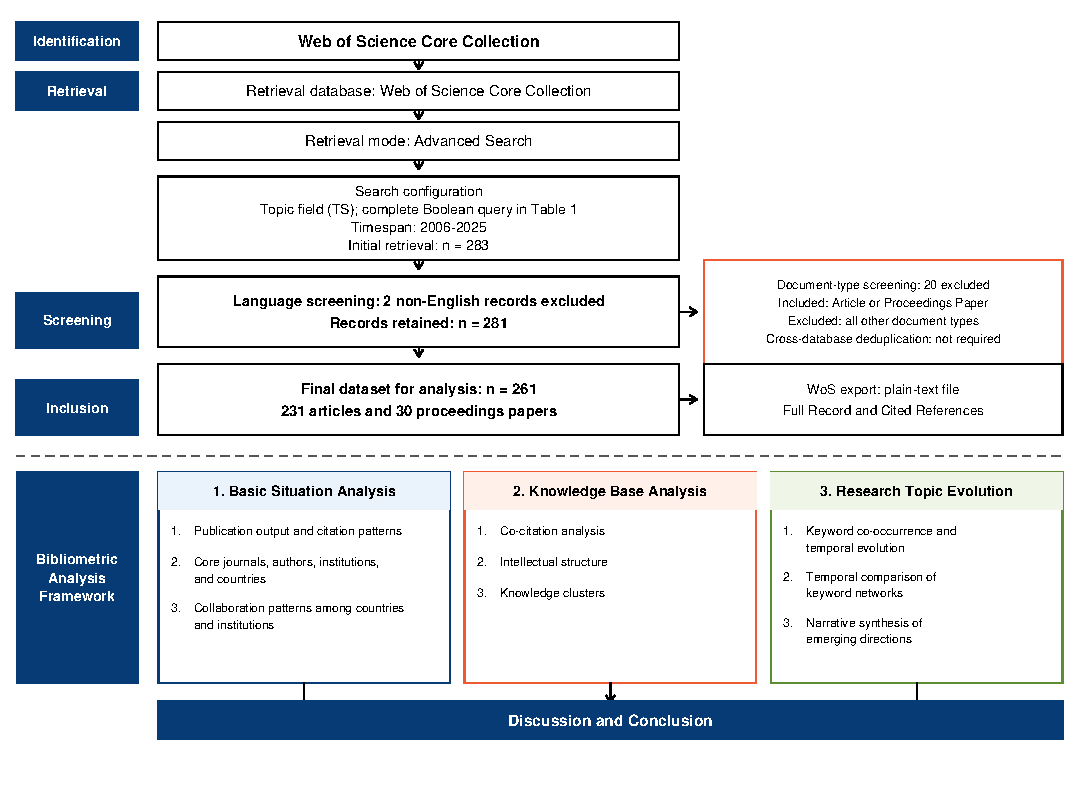
\includegraphics[width=0.9\linewidth]{Figures/flowchart.pdf} 
	\caption{\DIFdel{Flowchart} \DIFdel{of} \DIFdel{the} \DIFdel{research} \DIFdel{on} \DIFdel{technological} \DIFdel{development} \DIFdel{in} \DIFdel{LULC}\hspace{0.33em}\DIFadd{Workflow} \DIFadd{for} \DIFadd{literature} \DIFadd{retrieval}\DIFadd{,} \DIFadd{bibliometric} \DIFadd{analysis}\DIFadd{,} \DIFadd{and} \DIFadd{technical} \DIFadd{synthesis}.}
	\label{fig:flowchart}
\end{figure}


\section{Basic Situation Analysis}
\subsection{Yearly Output}

\begin{figure}[htb!]
	\centering
	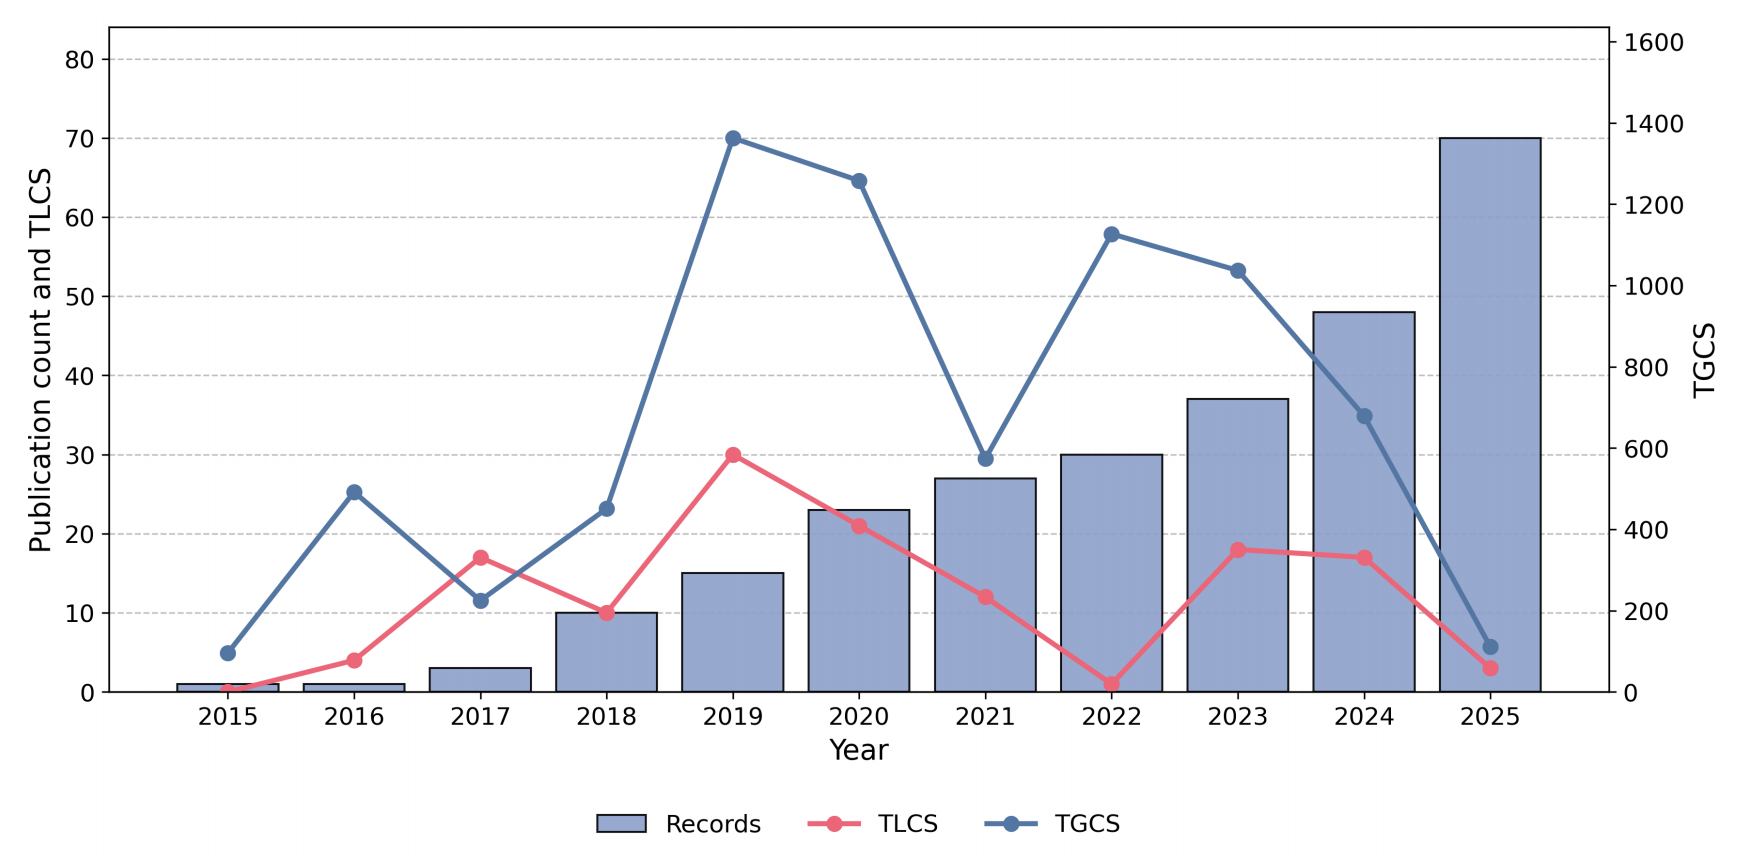
\includegraphics[width=0.75\columnwidth]{picture_2.png}
	\caption{Yearly publication output, TLCS, and TGCS \DIFdel{of} \DIFdel{LULC} \DIFdel{research} \DIFadd{for} \DIFadd{the} \DIFadd{retrieved} \DIFadd{corpus} (\DIFdel{2016--2025}\hspace{0.33em}\DIFadd{2015--2025})\DIFadd{;} \DIFadd{no} \DIFadd{records} \DIFadd{were} \DIFadd{retrieved} \DIFadd{for} \DIFadd{2006--2014}.}
	\label{fig:pub_trends}
\end{figure}

The period 2006--2014 is not explicitly detailed in the figure \DIFdel{due} \DIFdel{to} \DIFdel{the} \DIFdel{negligible} \DIFdel{number} \DIFdel{of} \DIFadd{because} \DIFadd{no} publications \DIFadd{were} \DIFadd{retrieved}; however, the single relevant paper published in 2015 is included to mark the onset of research growth. As shown in the figure, the annual volume of publications has exhibited a consistent upward trend. This growth \DIFdel{is} \DIFdel{primarily} \DIFdel{attributed} \DIFdel{to} \DIFadd{coincided} \DIFadd{with} the rapid advancement of deep learning algorithms and the continuous enhancement of computational power {\hypersetup{citecolor=red}\color{red}\citep{ORIGma2019deep}} {\color{blue}\citep{56}}. Notably, the final three years (2023--2025) represent the peak of productivity \DIFadd{in} \DIFadd{the} \DIFadd{retrieved} \DIFadd{corpus}, with 37, 48, and 70 papers published, respectively {\hypersetup{citecolor=red}\color{red}\citep{ORIGtuia2023toward}}\DIFadd{.} \DIFadd{This} \DIFadd{trend} \DIFadd{does} \DIFadd{not} \DIFadd{establish} \DIFadd{the} \DIFadd{share} \DIFadd{of} \DIFadd{fusion} \DIFadd{research} \DIFadd{in} \DIFadd{the} \DIFadd{broader} \DIFadd{LULC} \DIFadd{literature}.

While publication volume is \DIFdel{a} \DIFdel{reliable} \DIFadd{an} indicator of research activity, it does not fully capture academic influence. To address this, TLCS and TGCS based on citation counts are employed to gauge scholarly impact. Notably, TGCS values are generally \DIFdel{significantly} higher than TLCS, as they encompass citations from the entire Web of Science database rather than just within the selected local dataset {\hypersetup{citecolor=red}\color{red}\citep{ORIGbornmann2011citation}} {\color{blue}\citep{bornmann2011citation}}.

TLCS reached its peak in 2019 (30), indicating that papers published in this year have attracted substantial attention within the \DIFdel{specialized} \DIFdel{LULC} \DIFdel{community} \DIFadd{selected} \DIFadd{corpus}. Analysis reveals that two highly cited papers were the primary contributors to this peak: ``Advanced Multi-Sensor Optical Remote Sensing for Urban Land Use and Land Cover Classification: Outcome of the 2018 IEEE GRSS Data Fusion Contest'' (TLCS=17) \citep{21} and ``Combining Sentinel-1 and Sentinel-2 Satellite Image Time Series for land cover mapping via a multi-source deep learning architecture'' (TLCS=8) \citep{22}. Furthermore, although 2017 had a lower volume of publications, it maintained a relatively high TLCS. This is largely due to the \DIFdel{influential} work ``Hyperspectral and LiDAR Data Fusion Using Extinction Profiles and Deep Convolutional Neural Network'' (TLCS=15) \citep{23}. \DIFdel{Given} \DIFdel{that} \DIFdel{deep} \DIFdel{learning} \DIFadd{Annual} \DIFadd{citation} \DIFadd{totals} \DIFadd{can} \DIFadd{be} \DIFadd{concentrated} \DIFadd{in} \DIFadd{a} \DIFadd{small} \DIFadd{number} \DIFadd{of} \DIFadd{papers} and \DIFdel{multi-source} \DIFdel{fusion} are \DIFdel{contemporary} \DIFdel{research} \DIFdel{hotspots}\DIFdel{,} \DIFdel{these} \DIFdel{studies} \DIFdel{have} \DIFdel{naturally} \DIFdel{attracted} \DIFdel{extensive} \DIFdel{attention} \DIFadd{affected} \DIFadd{by} \DIFadd{publication} \DIFadd{age} \DIFadd{and} \DIFadd{citation} \DIFadd{practices}.

TGCS similarly peaked in 2019 (1363), driven by the aforementioned works and complemented by ``Urban Tree Species Classification Using a WorldView-2/3 and LiDAR Data Fusion Approach and Deep Learning'' {\hypersetup{citecolor=red}\color{red}\citep{ORIG26}} {\color{blue}\citep{26}}. A secondary peak in TGCS occurred in 2020 (1258)\DIFdel{,} \DIFdel{aligning} \DIFdel{with} \DIFdel{the} \DIFdel{TLCS} \DIFdel{trend}. In this year, ``Cloud removal in Sentinel-2 imagery using a deep residual neural network and SAR-optical data fusion'' \citep{27} contributed \DIFdel{significantly} \DIFdel{with} 345 global citations. Interestingly, despite a very low publication count in 2016, the year achieved a \DIFdel{remarkably} high TGCS due to the \DIFdel{seminal} work ``Deep Learning Earth Observation Classification Using ImageNet Pretrained Networks'' \citep{28}, which contributed 492 citations.

\DIFdel{It} \DIFdel{is} \DIFdel{obvious} \DIFdel{that} \DIFdel{high-impact}

\DIFadd{Within} \DIFadd{this} \DIFadd{deliberately} \DIFadd{focused} \DIFadd{corpus}\DIFadd{,} \DIFadd{several} \DIFadd{highly} \DIFadd{cited} studies \DIFdel{consistently} \DIFdel{focus} \DIFdel{on} \DIFadd{concern} the intersection of deep learning and multi-source fusion. We also observe local peaks in the 2023 TLCS and 2022 TGCS following minor declines, which may be attributed to the delayed citation window effect {\hypersetup{citecolor=red}\color{red}\citep{ORIG4,ORIGbornmann2011citation}} {\color{blue}\citep{bornmann2011citation}}. Conversely, the scores for 2024 and 2025 remain relatively low, as newly published papers typically require several years to accumulate significant citation counts.


\subsection{Core Journals, Authors, Institutions, and Countries}

\subsubsection{Active Journals}


Scientific journals serve as the primary conduits for disseminating research findings and academic activities. The 261 publications \DIFdel{analyzed} \DIFadd{analysed} in this study were distributed across 81 different journals. The top ten journals ranked by publication count, Local Citation Score (TLCS), and Total Global Citation Score (TGCS) are \DIFdel{summarized} \DIFadd{summarised} in Fig.~\ref{fig:journal_impact}.
\begin{figure}[htb!] 
	\centering
	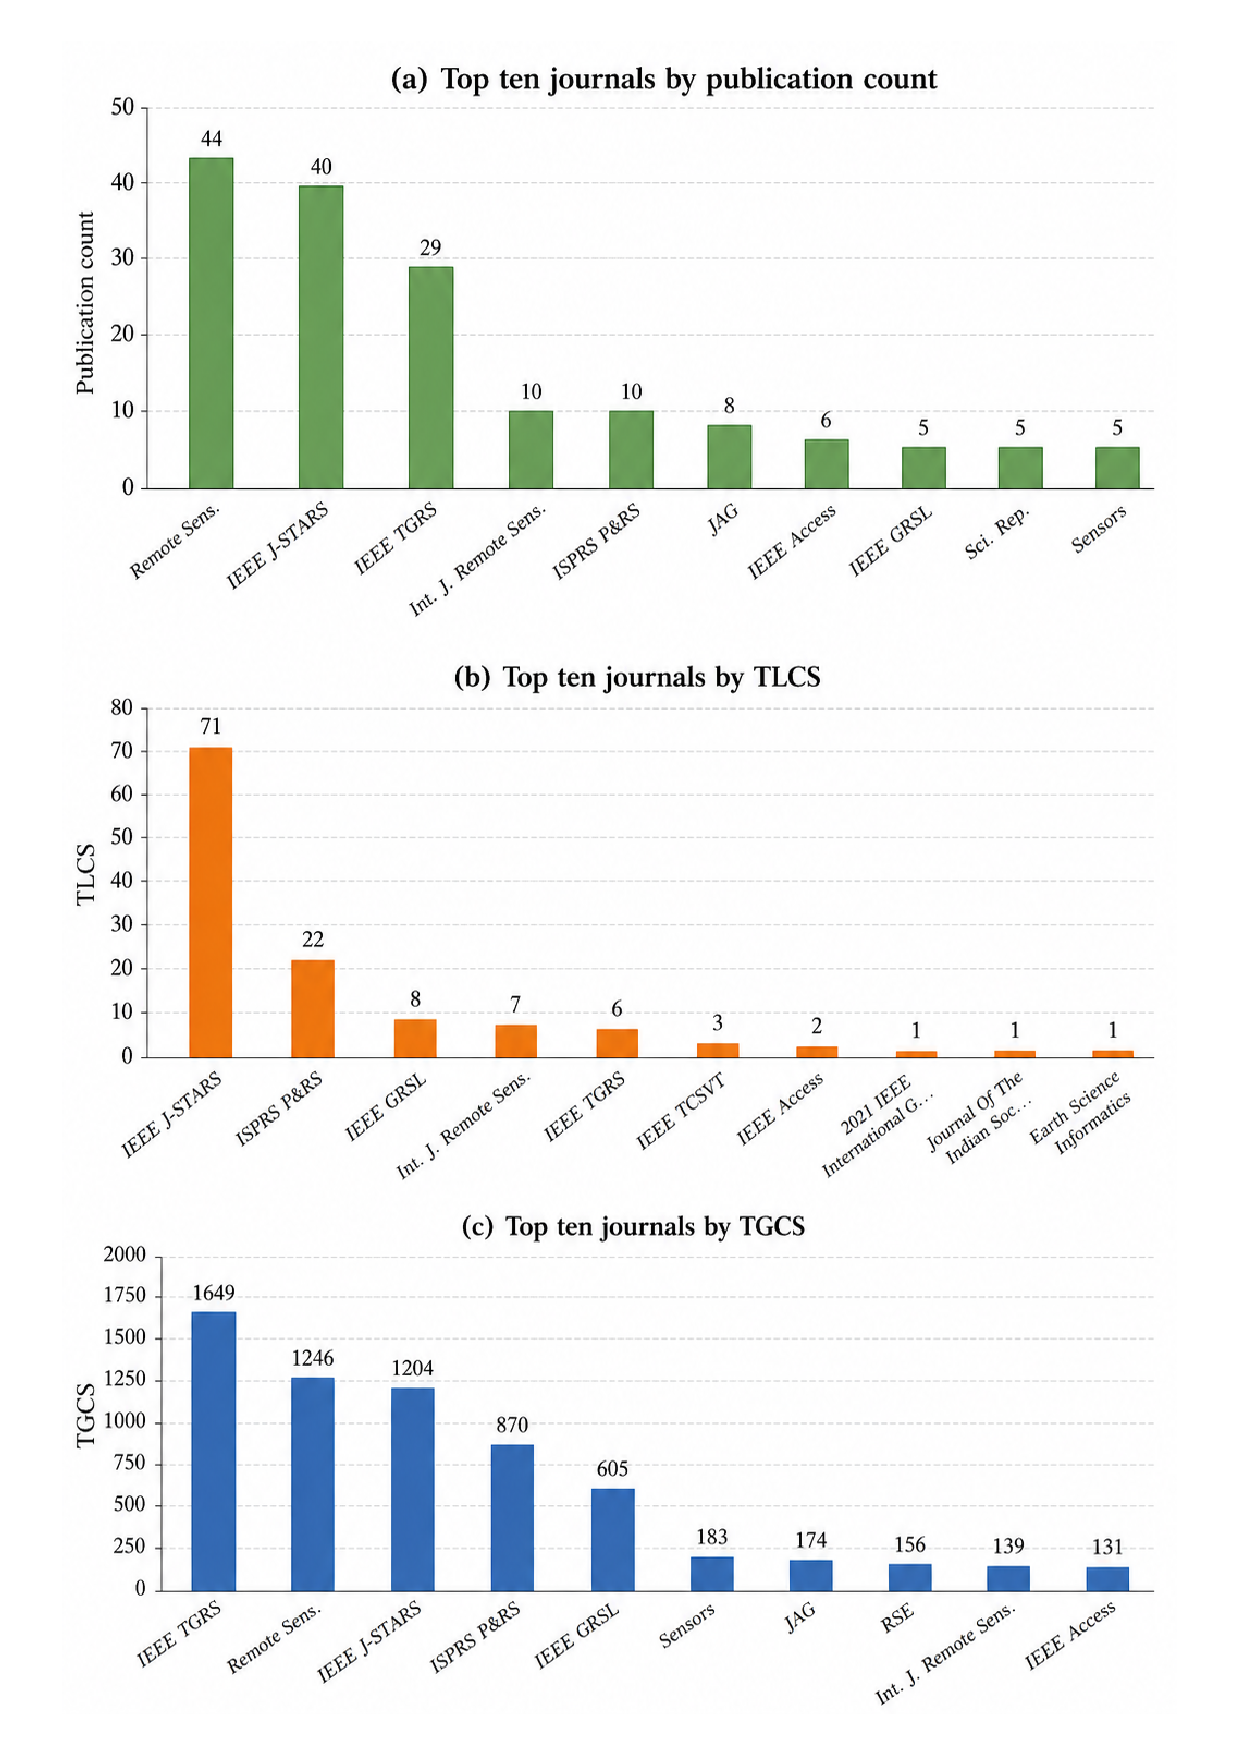
\includegraphics[width=0.67\columnwidth]{Figures/Picture_3.pdf} 
	\caption{Publication count, TLCS, and TGCS per journal (2006--2025).}
	\label{fig:journal_impact}
\end{figure}


According to Fig.~\ref{fig:journal_impact}(a), \textit{Remote Sensing} ranks first in terms of publication volume, making it the most active journal \DIFdel{in} \DIFadd{within} the \DIFdel{LULC} \DIFdel{research} \DIFdel{domain} \DIFadd{retrieved} \DIFadd{corpus}. However, its TLCS (7) only ranks fourth, \DIFdel{showing} \DIFdel{a} \DIFdel{significant} \DIFdel{discrepancy} compared to its \DIFdel{high} TGCS (1246). \DIFdel{This} \DIFdel{may} \DIFdel{be} \DIFdel{attributed} \DIFdel{to} \DIFdel{its} \DIFdel{status} \DIFdel{as} \DIFadd{These} \DIFadd{indicators} \DIFadd{use} \DIFadd{different} \DIFadd{citation} \DIFadd{populations}\DIFadd{;} \DIFadd{the} \DIFadd{observed} \DIFadd{difference} \DIFadd{does} \DIFadd{not} \DIFadd{establish} an \DIFdel{open-access} \DIFadd{effect} \DIFadd{of} \DIFadd{open} \DIFadd{access} \DIFadd{or} journal \DIFdel{with} \DIFdel{a} \DIFdel{broad} \DIFdel{and} \DIFdel{multidisciplinary} scope \DIFdel{(}\DIFdel{covering} \DIFdel{ecology}\DIFdel{,} \DIFdel{agriculture}\DIFdel{,} \DIFdel{hydrology}\DIFdel{,} \DIFdel{etc}\DIFdel{.}\DIFdel{)}\DIFdel{.} \DIFdel{Consequently}\DIFdel{,} \DIFdel{only} \DIFdel{a} \DIFdel{fraction} \DIFdel{of} \DIFdel{its} \DIFdel{total} \DIFdel{papers}\DIFdel{,} \DIFdel{those} \DIFdel{highly} \DIFdel{aligned} \DIFdel{with} \DIFdel{deep} \DIFdel{learning} \DIFdel{and} \DIFdel{remote} \DIFdel{sensing} \DIFdel{processing}\DIFdel{,} \DIFdel{are} \DIFdel{cited} \DIFdel{within} \DIFdel{this} \DIFdel{local} \DIFdel{sample} \DIFdel{set} \DIFdel{(}\DIFdel{low} \DIFdel{TLCS}\DIFdel{)}\DIFdel{,} \DIFdel{whereas} \DIFdel{its} \DIFdel{wide} \DIFdel{global} \DIFdel{audience} \DIFdel{leads} \DIFdel{to} \DIFdel{high} \DIFdel{cross-disciplinary} \DIFdel{citations} \DIFdel{(}\DIFdel{high} \DIFdel{TGCS}\DIFdel{)}.

In contrast, \textit{IEEE J-STARS} ranks first in TLCS and third in TGCS (Fig.~\ref{fig:journal_impact}(b, c)), \DIFdel{indicating} \DIFdel{that} \DIFdel{its} \DIFdel{publications} \DIFdel{are} \DIFdel{not} \DIFdel{only} \DIFdel{highly} \DIFdel{cited} within the \DIFdel{LULC} \DIFdel{community} \DIFdel{but} \DIFdel{also} \DIFdel{attract} \DIFdel{extensive} \DIFdel{attention} \DIFdel{from} \DIFdel{the} \DIFdel{broader} \DIFdel{scientific} \DIFdel{world} \DIFadd{retrieved} \DIFadd{corpus}. Furthermore, \textit{IEEE TGRS} leads in TGCS (1649), \DIFdel{which} \DIFdel{is} \DIFdel{consistent} \DIFdel{with} \DIFdel{its} \DIFdel{reputation} \DIFdel{as} \DIFdel{one} \DIFdel{of} \DIFdel{the} \DIFdel{oldest} \DIFadd{although} \DIFadd{raw} \DIFadd{citation} \DIFadd{totals} \DIFadd{are} \DIFadd{influenced} \DIFadd{by} \DIFadd{publication} \DIFadd{age} and \DIFdel{most} \DIFdel{prestigious} \DIFdel{top-tier} \DIFdel{journals} \DIFdel{in} \DIFdel{the} \DIFdel{remote} \DIFdel{sensing} \DIFdel{field} \DIFdel{since} \DIFdel{1963} \DIFadd{a} \DIFadd{few} \DIFadd{highly} \DIFadd{cited} \DIFadd{papers}.


\subsubsection{Important Authors}

Identifying key authors helps researchers grasp research hotspots and academic trends. In this study, 1,083 authors contributed to the 261 \DIFdel{analyzed} \DIFadd{analysed} papers. The authors were ranked based on publication count, TLCS, and TGCS, as illustrated in Fig.~\ref{fig:author_impact}. 


\begin{figure}[htb!] 
	\centering
	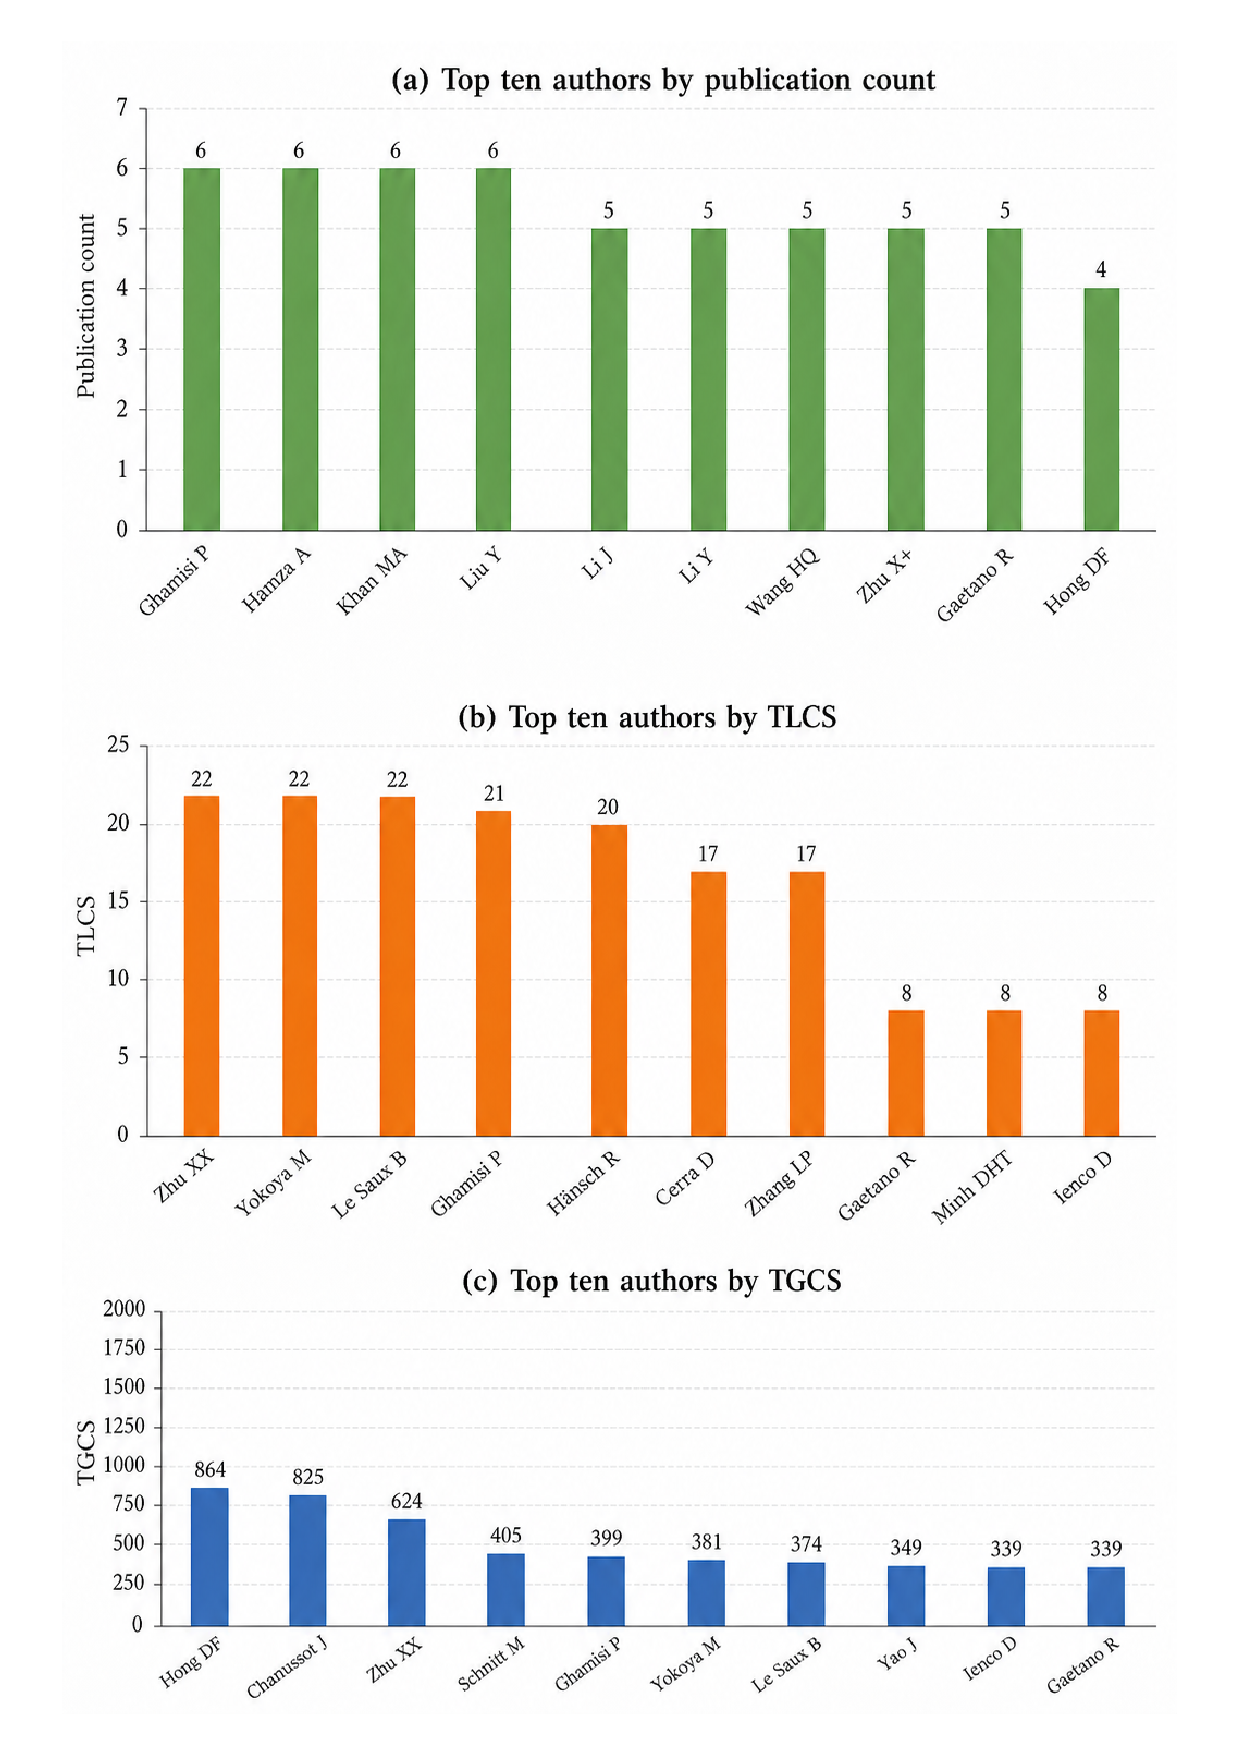
\includegraphics[width=0.67\columnwidth]{Figures/Picture_4.pdf} 
	\caption{Publication count, TLCS, and TGCS per author \DIFdel{for} \DIFdel{LULC} \DIFdel{research} \DIFadd{within} \DIFadd{the} \DIFadd{retrieved} \DIFadd{corpus} (2006--2025).}
	\label{fig:author_impact}
\end{figure}

While Ghamisi P., Hamza A., Khan M. A., and Liu Y. lead in publication count with six papers each, further analysis of Fig.~\ref{fig:author_impact} (b, c) reveals that only Ghamisi P. maintains a top-ten ranking in both TLCS (5th, 21) and TGCS (5th, 399). This demonstrates his \DIFdel{significant} \DIFdel{contribution} \DIFdel{to} \DIFadd{citation} \DIFadd{impact} \DIFadd{within} both the local \DIFdel{community} \DIFadd{corpus} and \DIFdel{global} \DIFdel{impact} \DIFadd{the} \DIFadd{wider} \DIFadd{Web} \DIFadd{of} \DIFadd{Science} \DIFadd{database}. Notably, Zhu X. X., Yokoya N., and Le Saux B. also exhibit high TLCS values (22 each). The collaborative work by Ghamisi P. and Zhu X. X., ``Hyperspectral and LiDAR Data Fusion Using Extinction Profiles and Deep Convolutional Neural Network'' \citep{23}, contributed a notable TLCS of 15. \DIFdel{The} \DIFdel{frequent} \DIFdel{collaboration} \DIFdel{between} \DIFdel{these} \DIFdel{two} \DIFdel{authors} \DIFdel{and} \DIFdel{others} \DIFdel{highlights} \DIFdel{their} \DIFdel{roles} \DIFdel{as} \DIFdel{influential} \DIFdel{academic} \DIFdel{partners}\DIFdel{.} \DIFdel{From} \DIFdel{a} \DIFdel{global} \DIFdel{perspective}\DIFdel{,} Hong D. F. shows the \DIFdel{greatest} \DIFdel{influence} \DIFadd{highest} \DIFadd{TGCS} in \DIFdel{TGCS} \DIFadd{the} \DIFadd{retrieved} \DIFadd{corpus}, primarily due to the work of 2022 ``Convolutional Neural Networks for Multimodal Remote Sensing Data Classification'' \citep{2}, which achieved a TGCS of 450.


\subsubsection{Active Institutions and Main Countries}
Institutions play a pivotal role in \DIFdel{analyzing} \DIFdel{global} \DIFadd{analysing} developmental trends within \DIFdel{a} \DIFdel{specific} \DIFdel{academic} \DIFdel{field} \DIFadd{the} \DIFadd{retrieved} \DIFadd{LULC} \DIFadd{literature}. By calculating the affiliations of all authors, a total of 420 institutions were identified. The statistical results for publication volume, Local Citation Score (TLCS), and Total Global Citation Score (TGCS) for each institution are \DIFdel{summarized} \DIFadd{summarised} in Fig.~\ref{fig:inst_impact}. Wuhan University leads with 24 publications, making it the most active institution \DIFdel{in} \DIFdel{this} \DIFdel{field} \DIFadd{within} \DIFadd{the} \DIFadd{retrieved} \DIFadd{corpus}. The Chinese Academy of Sciences (CAS) and Huazhong University of Science and Technology follow in second and third place, with 22 and 10 publications, respectively. Notably, the output from Wuhan University and CAS \DIFdel{significantly} exceeds that of \DIFadd{the} other \DIFadd{listed} institutions.


In terms of TLCS rankings, the German Aerospace Center (DLR) and Zhuhai University hold prominent positions. Wuhan University, \DIFadd{the} \DIFadd{Pakistan} \DIFadd{Institute} \DIFadd{of} \DIFadd{Engineering} \DIFadd{and} \DIFadd{Applied} \DIFadd{Sciences} \DIFadd{(}PIEAS\DIFadd{)}, and \DIFadd{the} University of Technology Sydney follow closely, each with a TLCS of 22. These results indicate that Wuhan University not only maintains high \DIFdel{annual} \DIFadd{publication} output but also \DIFdel{commands} \DIFdel{significant} \DIFdel{academic} \DIFdel{recognition} \DIFadd{receives} \DIFadd{substantial} \DIFadd{citation} \DIFadd{attention} within the \DIFdel{field} \DIFadd{analysed} \DIFadd{corpus}. Regarding TGCS (as shown in Fig.~\ref{fig:inst_impact}(c)), CAS and Zhejiang University \DIFdel{emerge} \DIFdel{as} \DIFadd{have} the \DIFdel{leading} \DIFdel{global} \DIFdel{institutions} \DIFadd{highest} \DIFadd{TGCS} \DIFadd{values} \DIFadd{in} \DIFadd{the} \DIFadd{retrieved} \DIFadd{corpus}. 


National contribution is another critical dimension for assessing academic activity in LULC. The retrieved literature spans 134 countries\DIFdel{,} \DIFdel{demonstrating} \DIFdel{the} \DIFdel{worldwide} \DIFdel{importance} \DIFdel{of} \DIFdel{this} \DIFdel{field}. The top ten countries by publication volume account for 89.30\% of the total output. Fig.~\ref{fig:country_impact} illustrates the distribution of the top ten countries across the three metrics: publication count, TLCS, and TGCS. Germany and China rank within the top three across all three metrics. However, raw publication counts do not fully reflect national research intensity; \DIFdel{contributions} \DIFdel{are} \DIFdel{better} \DIFdel{assessed} \DIFdel{relative} \DIFdel{to} population size\DIFadd{,} \DIFadd{research-system} \DIFadd{size}\DIFadd{,} \DIFadd{database} \DIFadd{coverage}\DIFadd{,} and \DIFdel{the} \DIFdel{number} \DIFadd{publication} \DIFadd{age} \DIFadd{can} \DIFadd{affect} \DIFadd{these} \DIFadd{indicators}\DIFadd{.} \DIFadd{No} \DIFadd{normalised} \DIFadd{comparison} of \DIFdel{active} \DIFdel{PhD} \DIFdel{researchers} \DIFdel{in} \DIFdel{each} \DIFdel{country}\DIFdel{.} \DIFdel{When} \DIFdel{these} \DIFdel{normalization} \DIFdel{factors} \DIFdel{are} \DIFdel{considered}\DIFdel{,} \DIFdel{the} \DIFdel{relative} \DIFdel{standing} \DIFdel{of} \DIFdel{some} \DIFdel{countries} \DIFdel{may} \DIFdel{shift}\DIFdel{.} \DIFdel{Furthermore}\DIFdel{,} \DIFdel{several} \DIFdel{prestigious} \DIFdel{institutions} \DIFdel{are} \DIFdel{based} \DIFdel{in} \DIFdel{these} \DIFdel{two} \DIFdel{nations}\DIFdel{,} \DIFdel{underscoring} \DIFdel{their} \DIFdel{dominant} \DIFdel{influence} \DIFdel{in} \DIFdel{both} \DIFdel{the} \DIFdel{local} \DIFdel{academic} \DIFdel{community} \DIFdel{and} \DIFdel{the} \DIFdel{global} \DIFdel{scientific} \DIFdel{sphere} \DIFadd{national} \DIFadd{research} \DIFadd{capacity} \DIFadd{was} \DIFadd{performed}. Six countries, including China, Germany, India, France, the UK, and Japan, consistently rank among the top ten across all indicators \DIFadd{in} \DIFadd{this} \DIFadd{corpus}. 


As shown in Figs.~\ref{fig:country_impact} and~\ref{fig:country_collab_compact}, China \DIFdel{holds} \DIFdel{an} \DIFdel{absolute} \DIFdel{leading} \DIFdel{position}\DIFdel{,} \DIFdel{with} \DIFdel{its} \DIFdel{total} \DIFadd{has} \DIFadd{the} \DIFadd{largest} publication \DIFdel{volume} \DIFdel{far} \DIFdel{exceeding} \DIFdel{that} \DIFdel{of} \DIFdel{other} \DIFdel{nations} \DIFadd{count} \DIFadd{in} \DIFadd{the} \DIFadd{retrieved} \DIFadd{corpus}. The \DIFdel{vast} majority of China's \DIFdel{research} \DIFdel{is} \DIFdel{conducted} \DIFdel{independently} \DIFdel{within} \DIFdel{the} \DIFdel{country} \DIFadd{records} \DIFadd{are} \DIFadd{single-country} \DIFadd{publications} (indicated by the large light-green portion in Fig.~\ref{fig:country_collab_compact}), while multi-country collaborative papers represent a smaller fraction. This spatial distribution is further elucidated in Fig.~\ref{fig:collab_map}, which \DIFdel{visualizes} \DIFadd{visualises} the intensity and geographical direction of these partnerships. \DIFdel{Despite} \DIFdel{the} \DIFdel{high} \DIFdel{proportion} \DIFdel{of} \DIFdel{independent} \DIFdel{research}\DIFdel{,} \DIFdel{China} \DIFdel{maintains} \DIFdel{a} \DIFdel{robust} \DIFdel{international} \DIFdel{network}\DIFdel{,} \DIFdel{with} \DIFdel{significant} Collaborative links \DIFdel{extending} \DIFdel{primarily} \DIFadd{extend} \DIFadd{from} \DIFadd{China} to \DIFadd{countries} \DIFadd{in} North America, Europe, and Australia \DIFadd{within} \DIFadd{this} \DIFadd{corpus}.

Other countries exhibit distinct collaboration patterns: India and Germany also show a high proportion of \DIFdel{independent} \DIFdel{research} \DIFadd{single-country} \DIFadd{publications}. In contrast, while the total publication volumes for the USA, South Korea, Iran, and Australia decrease sequentially, their proportion of international collaborative papers (indicated in red in Fig.~\ref{fig:country_collab_compact}) is \DIFdel{significantly} more prominent. As illustrated in the geographical distribution (Fig.~\ref{fig:collab_map}), these nations \DIFdel{act} \DIFdel{as} \DIFdel{key} \DIFdel{nodes} \DIFadd{have} \DIFadd{international} \DIFadd{collaborative} \DIFadd{links}\DIFadd{.} \DIFadd{These} \DIFadd{patterns} \DIFadd{describe} \DIFadd{co-authorship} in the \DIFdel{global} \DIFdel{LULC} \DIFadd{selected} \DIFadd{corpus} \DIFadd{and} \DIFadd{do} \DIFadd{not} \DIFadd{establish} \DIFadd{that} \DIFadd{collaboration} \DIFadd{increased} research \DIFdel{network}\DIFdel{,} \DIFdel{facilitating} \DIFdel{transcontinental} \DIFdel{knowledge} \DIFdel{flow} \DIFadd{quality} \DIFadd{or} \DIFadd{citation} \DIFadd{impact}. \DIFdel{This} \DIFdel{reflects} \DIFdel{that} \DIFdel{while} \DIFdel{China} \DIFdel{leads} \DIFdel{in} \DIFdel{volume} \DIFdel{through} \DIFdel{primarily} \DIFdel{independent} \DIFdel{research}\DIFdel{,} \DIFdel{followed} \DIFdel{by} \DIFdel{India} \DIFdel{and} \DIFdel{Germany}\DIFdel{,} \DIFdel{other} \DIFdel{nations} \DIFdel{leverage} \DIFdel{international} \DIFdel{cooperation} \DIFdel{more} \DIFdel{extensively} \DIFdel{to} \DIFdel{enhance} \DIFdel{their} \DIFdel{scientific} \DIFdel{impact} \DIFdel{and} \DIFdel{resource} \DIFdel{sharing}\DIFdel{.}

\begin{figure}[!htbp]
	\centering
	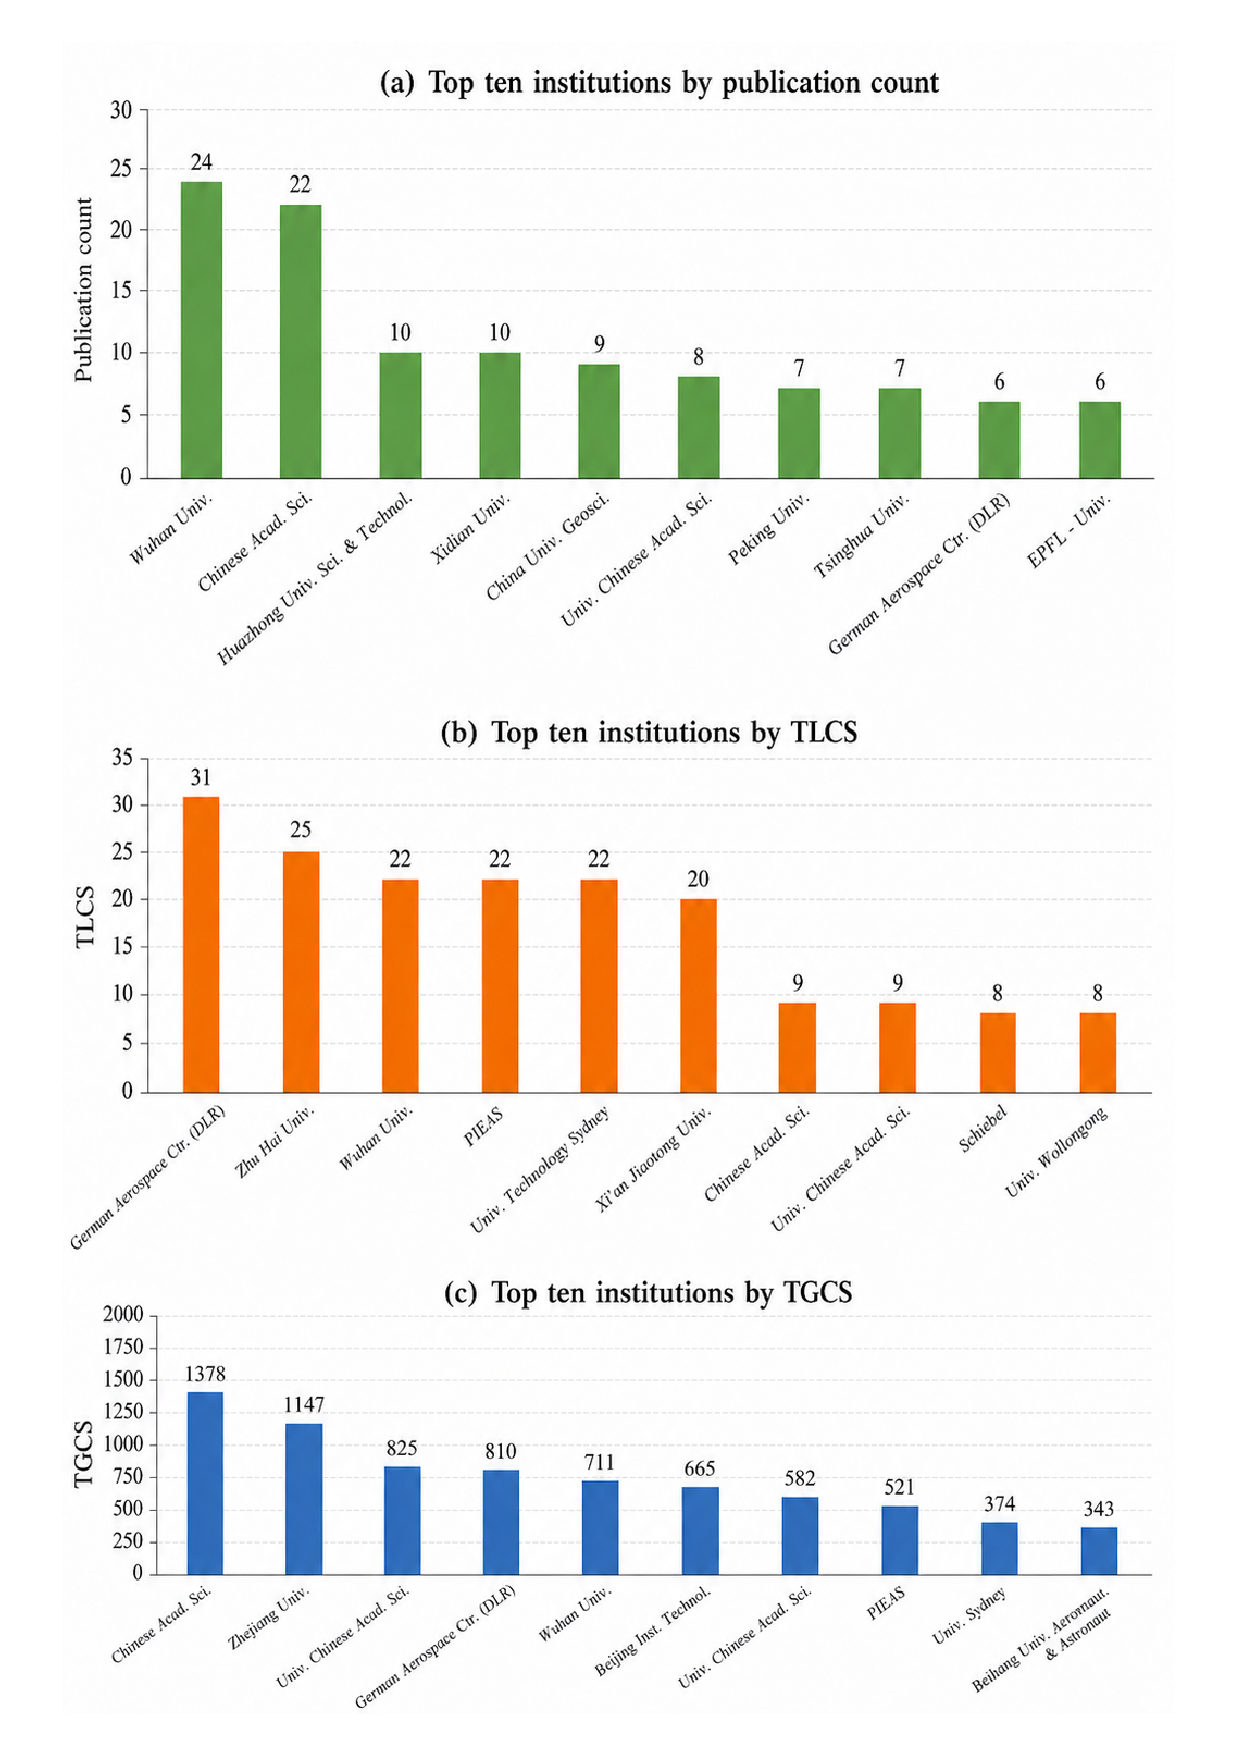
\includegraphics[width=0.67\columnwidth]{Figures/Picture_5.pdf} 
	\caption{Publication volume, TLCS, and TGCS per institution \DIFdel{for} \DIFdel{LULC} \DIFdel{research} \DIFadd{within} \DIFadd{the} \DIFadd{retrieved} \DIFadd{corpus} (2006--2025).}
	\label{fig:inst_impact}
\end{figure}




\begin{figure}[!htbp]
	\centering
	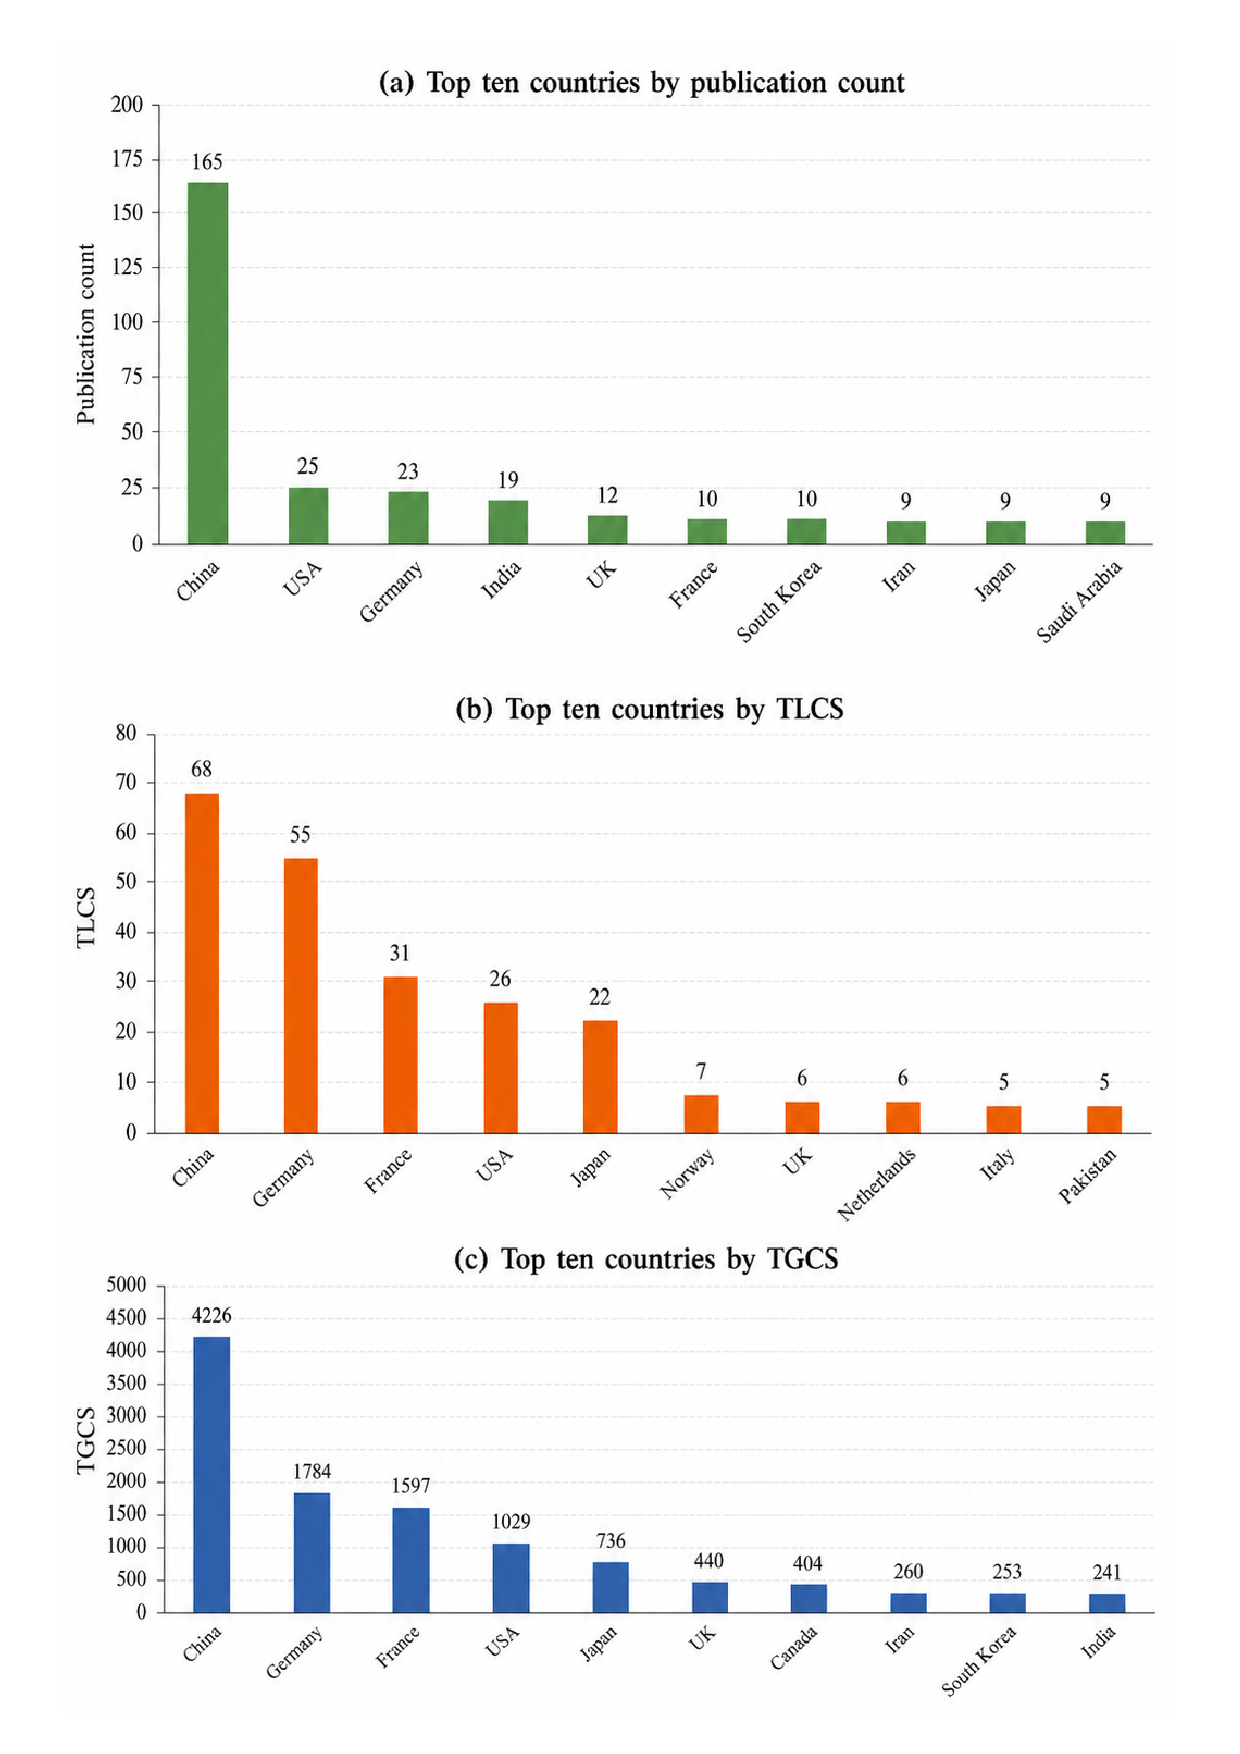
\includegraphics[width=0.67\columnwidth]{Figures/Picture_6.pdf} 
	\caption{Top ten countries ranked by publication volume, TLCS, and TGCS \DIFdel{for} \DIFdel{LULC} \DIFdel{research} \DIFadd{within} \DIFadd{the} \DIFadd{retrieved} \DIFadd{corpus} (2006--2025).}
	\label{fig:country_impact}
\end{figure}

\FloatBarrier

\begin{figure}[htb!]
	\centering	
	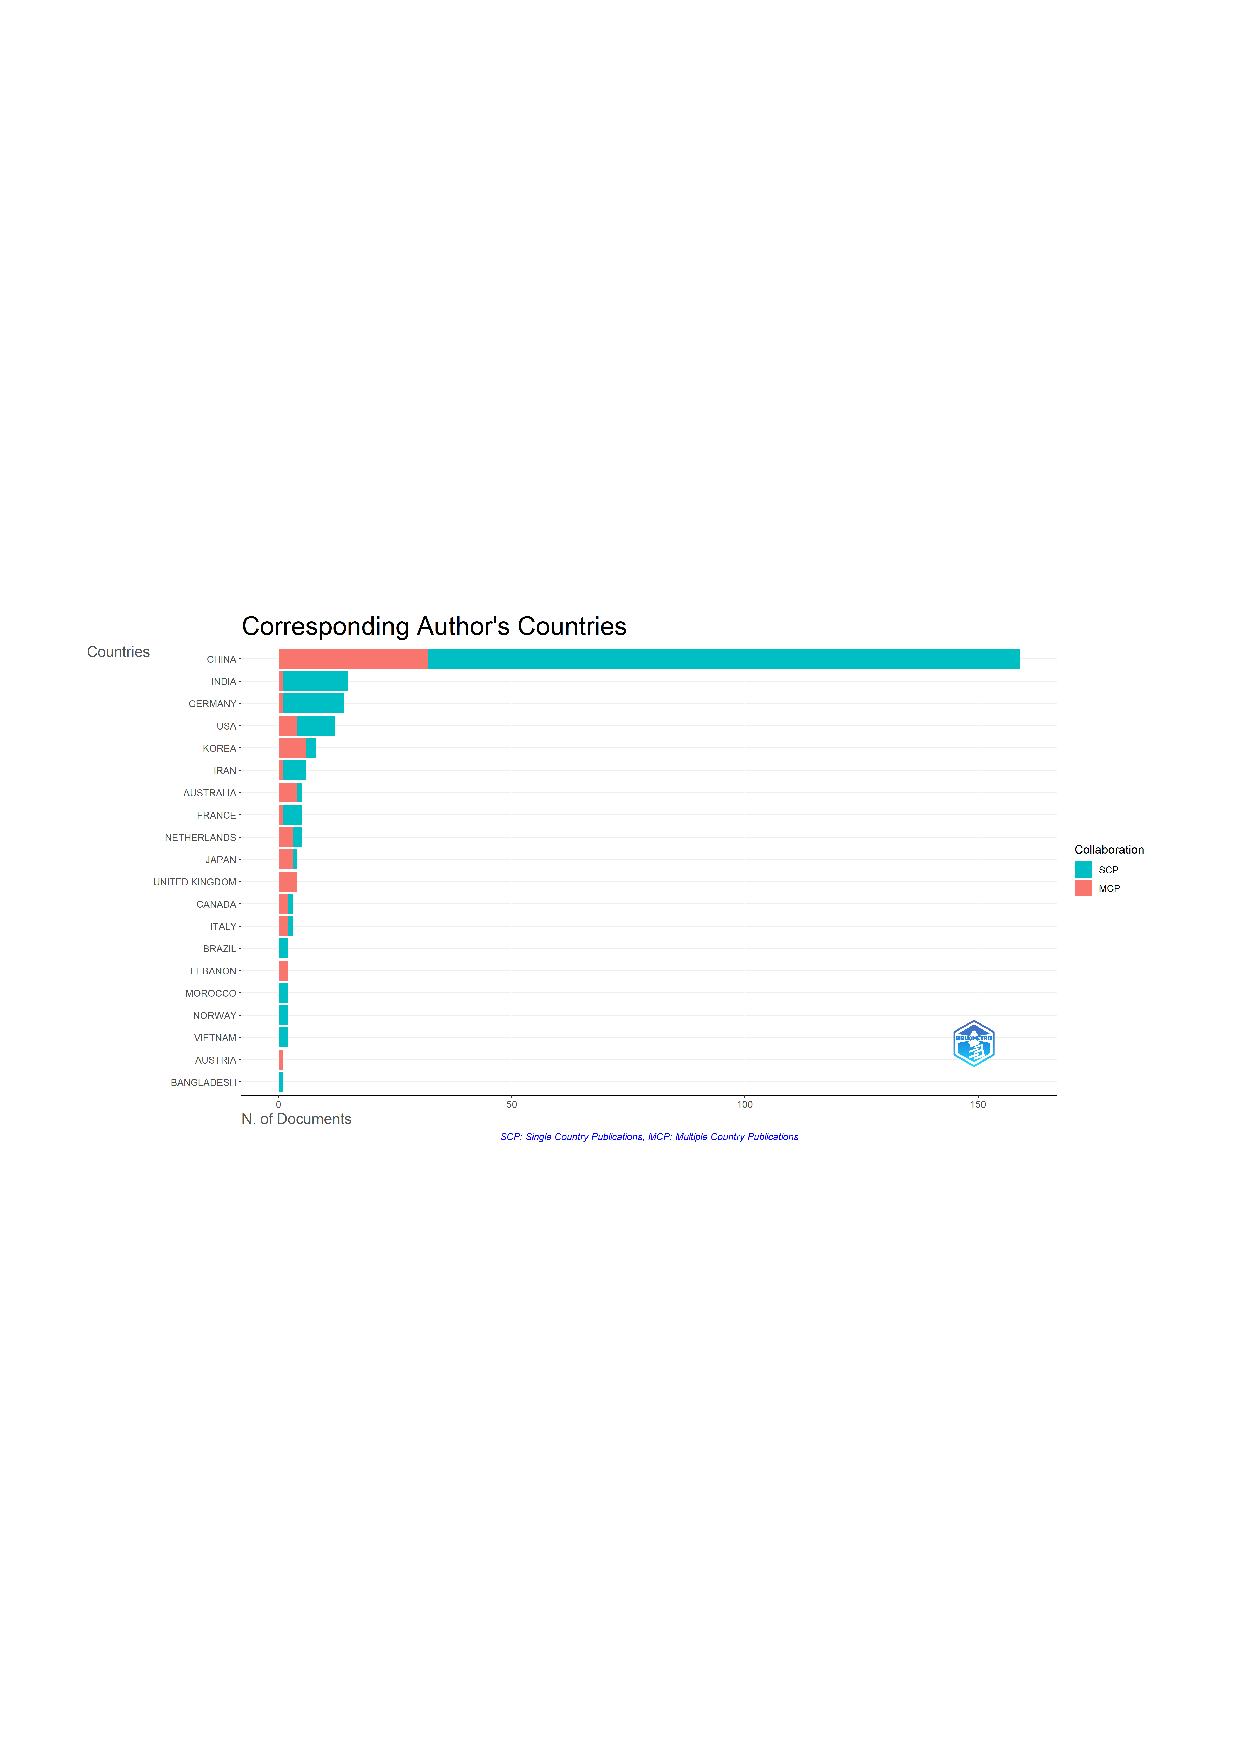
\includegraphics[width=1.0\textwidth, height=0.38\textheight, keepaspectratio]{Figures/picture_7.pdf}
	\vspace{-10pt}
	\caption{Collaboration analysis of major countries: MCP versus SCP. Here, MCP denotes Multiple Country Publication (i.e., co-authors from two or more different countries), while SCP denotes Single Country Publication (i.e., all authors affiliated with the same country)\DIFadd{.}}
	\label{fig:country_collab_compact}
	\vspace{10pt}
	
	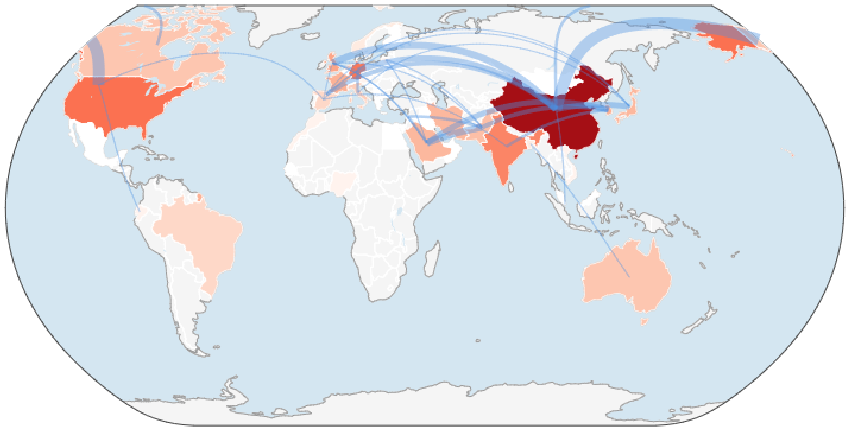
\includegraphics[width=\linewidth]{Figures/newplot_original_pdf_fig8.pdf}
	\vspace{-10pt}
	\caption{Geographical distribution of international research collaborations.}
	\label{fig:collab_map}
\end{figure}

\section{Results and Discussion}

\subsection{Keyword Co-occurrence and Temporal Evolution}

In this study, VOSviewer software was employed to conduct a keyword hotspot analysis on 261 publications related to LULC \DIFdel{simulation} \DIFadd{classification} indexed in the Web of Science database from 2006 to 2025. The analysis reveals the core research trends and \DIFadd{their} \DIFadd{temporal} \DIFadd{evolution} \DIFadd{within} the \DIFdel{evolutionary} \DIFdel{path} \DIFdel{of} \DIFdel{the} \DIFdel{field} \DIFadd{retrieved} \DIFadd{corpus}, as illustrated in Fig.~\ref{fig:keyword_evolution}. Notably, \DIFdel{due} \DIFdel{to} \DIFdel{the} \DIFdel{limited} \DIFdel{number} \DIFdel{of} \DIFdel{publications} \DIFdel{between} \DIFdel{2006} \DIFadd{because} \DIFadd{no} \DIFadd{records} \DIFadd{were} \DIFadd{retrieved} \DIFadd{for} \DIFadd{2006--2014} and \DIFadd{only} \DIFadd{one} \DIFadd{for} 2015, keyword \DIFdel{visualization} \DIFadd{visualisation} for that specific decade is omitted.

\begin{figure}[!htbp]
	\centering
	\subfloat[2016--2020]{%
		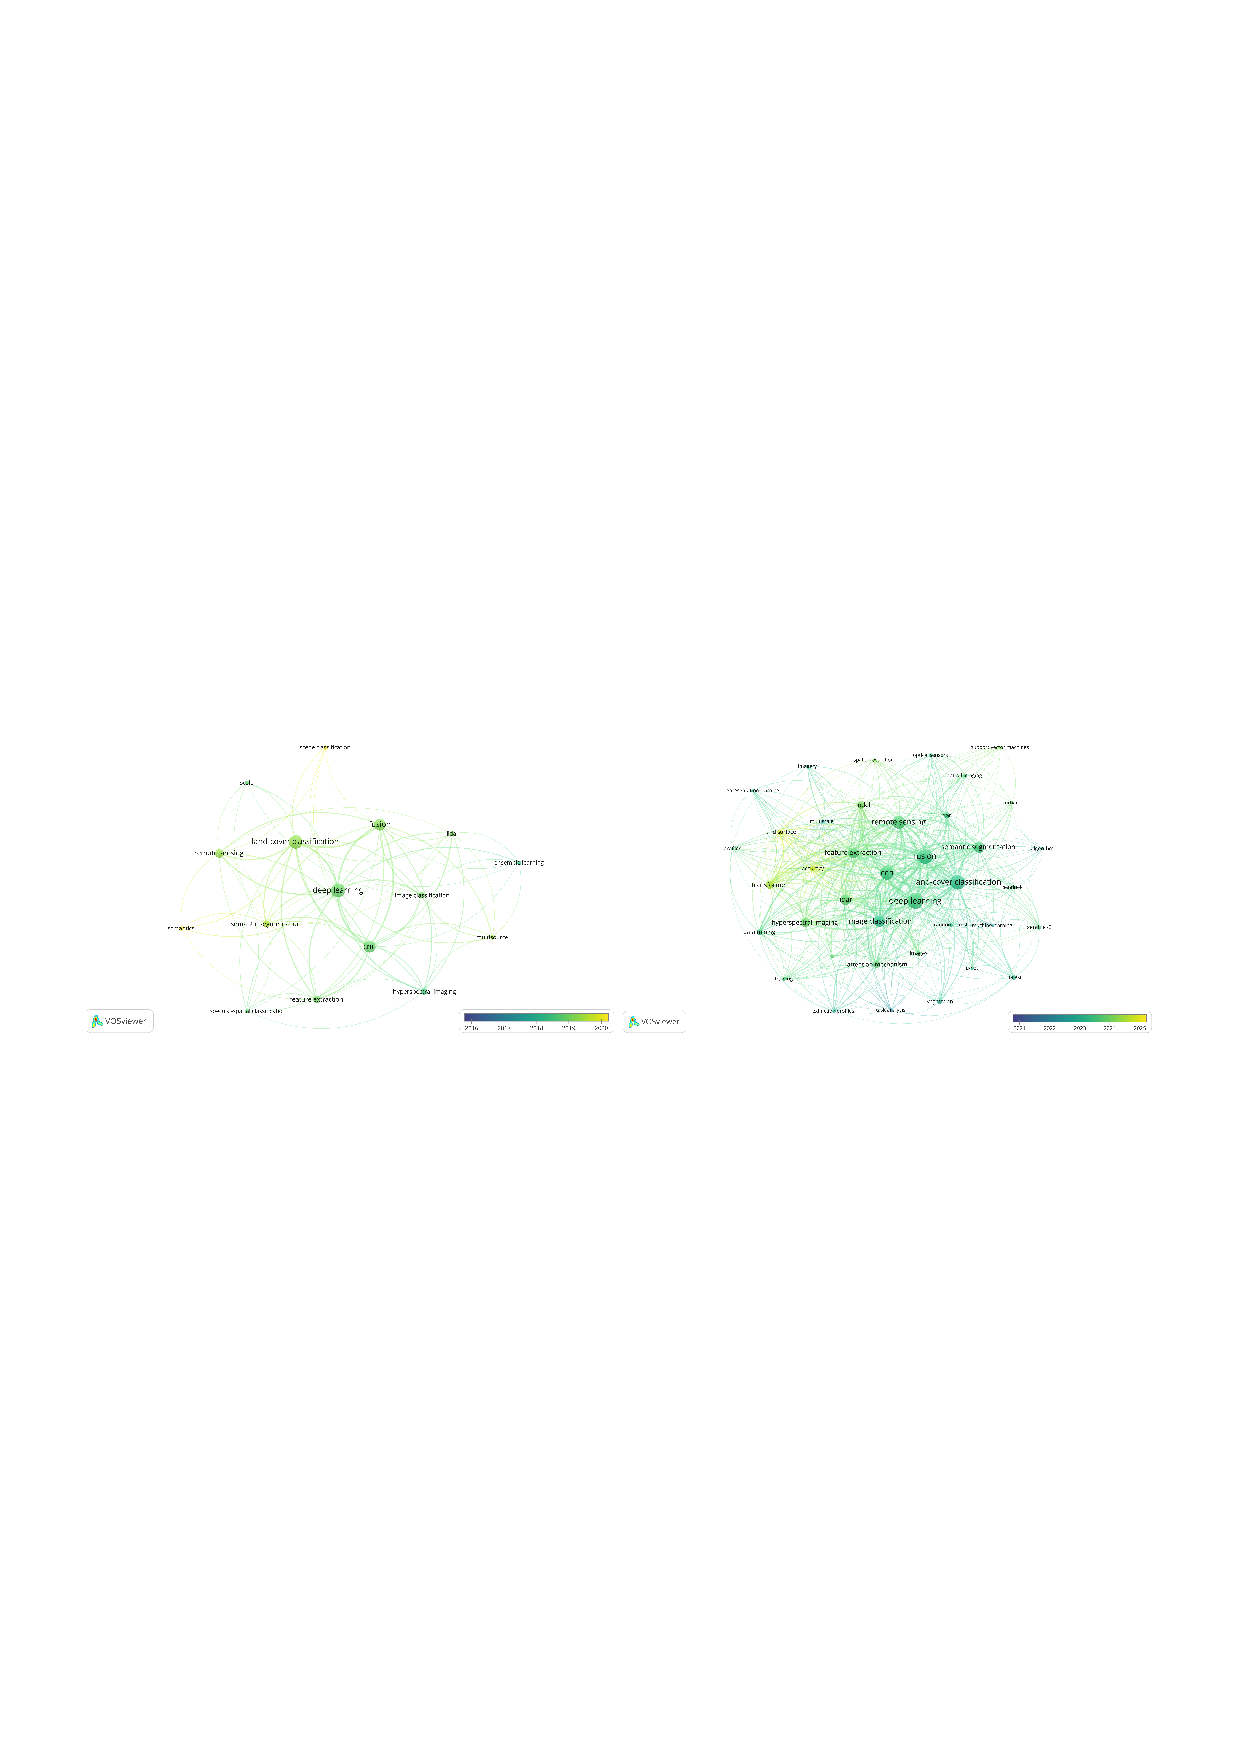
\includegraphics[
			width=0.96\linewidth,
			trim=0 0 256 0,
			clip
		]{Figures/picture_8.pdf}}
	\par\vspace{8pt}
	\subfloat[2021--2025]{%
		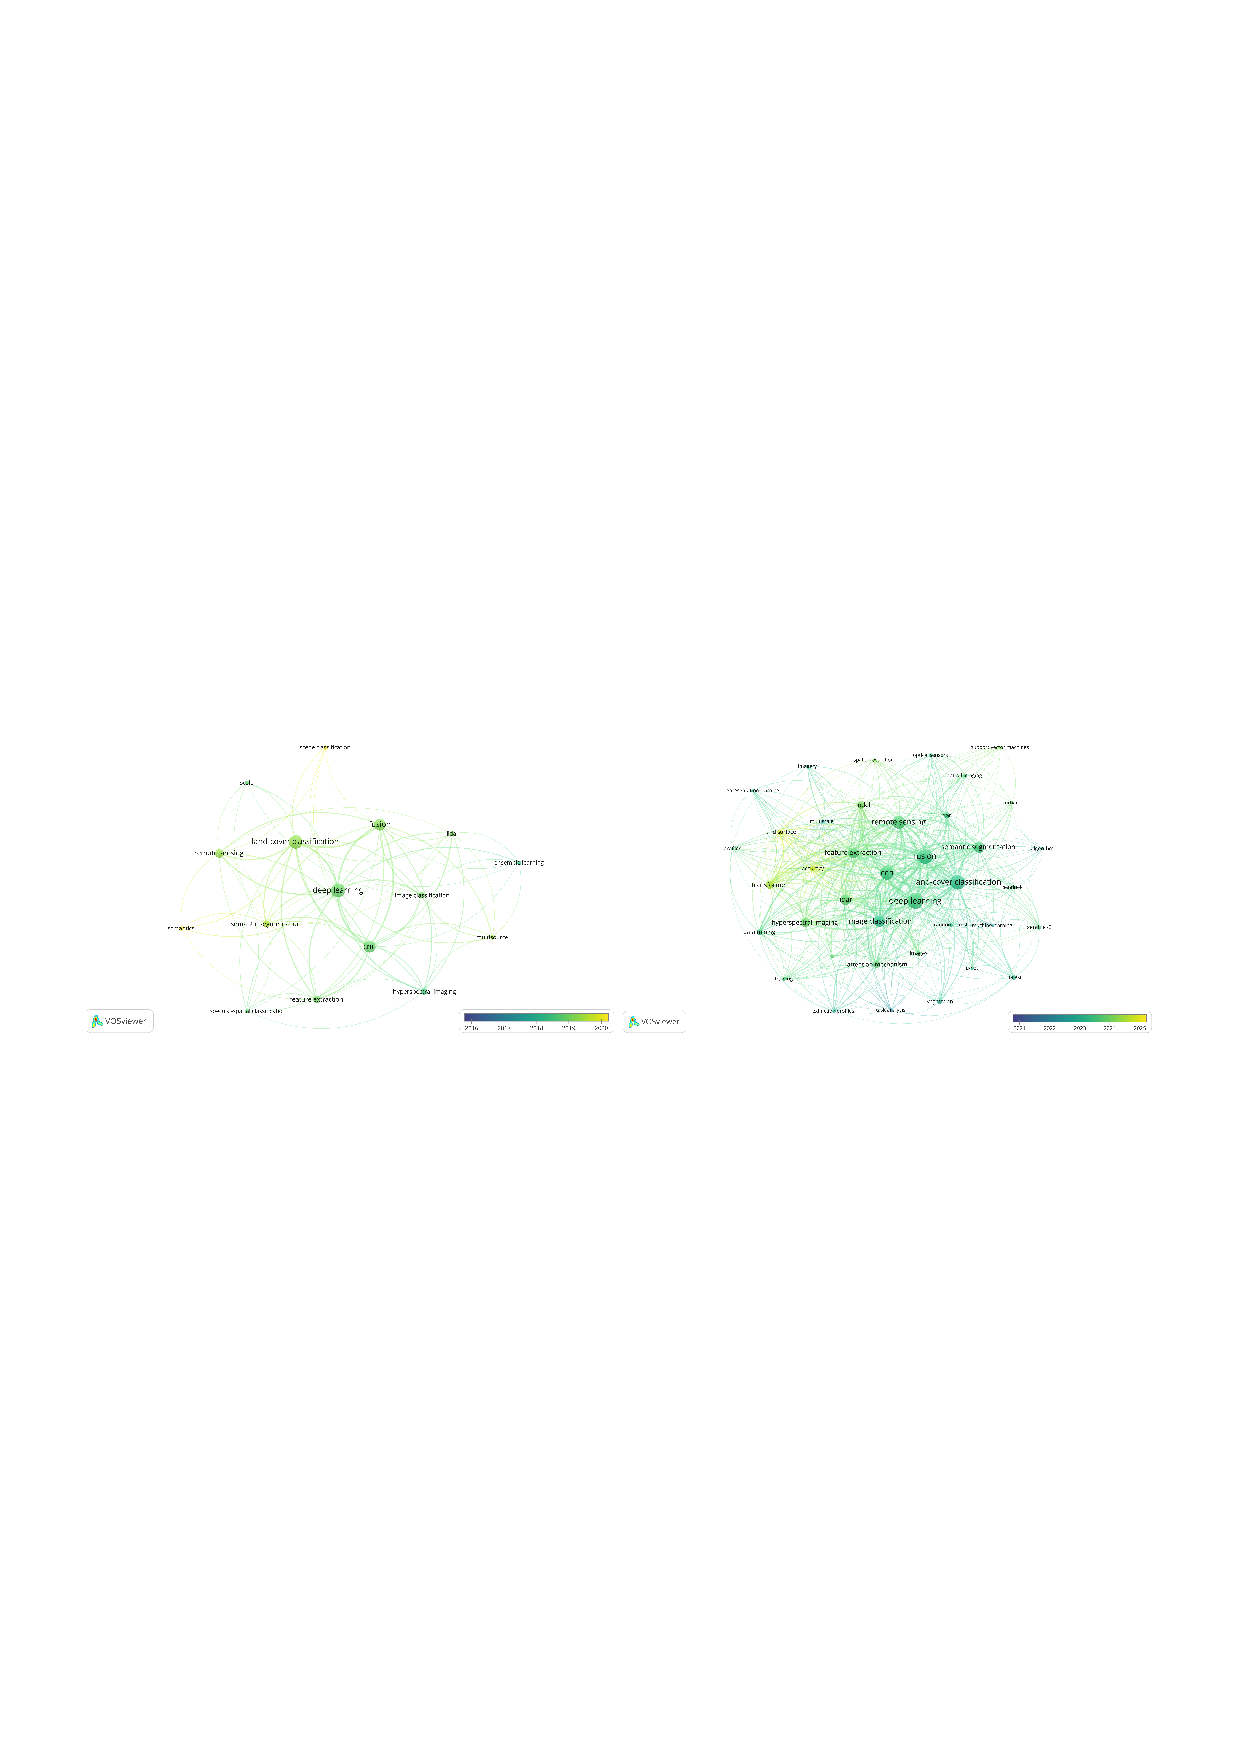
\includegraphics[
			width=0.96\linewidth,
			trim=256 0 0 0,
			clip
		]{Figures/picture_8.pdf}}
	\caption{\DIFadd{Keyword} \DIFadd{co-occurrence} \DIFadd{networks} \DIFadd{for} \DIFadd{the} \DIFadd{retrieved} \DIFadd{LULC} \DIFadd{classification} \DIFadd{literature}\DIFadd{:} \DIFadd{(}\DIFadd{a}\DIFadd{)} \DIFadd{2016--2020}\DIFadd{;} \DIFadd{(}\DIFadd{b}\DIFadd{)} \DIFadd{2021--2025}\DIFadd{.} \DIFadd{For} \DIFadd{readability}\DIFadd{,} \DIFadd{labels} \DIFadd{are} \DIFadd{displayed} \DIFadd{only} \DIFadd{for} \DIFadd{the} \DIFadd{more} \DIFadd{prominent} \DIFadd{nodes} \DIFadd{selected} \DIFadd{by} \DIFadd{the} \DIFadd{visualisation} \DIFadd{software}\DIFadd{;} \DIFadd{all} \DIFadd{retained} \DIFadd{nodes} \DIFadd{contribute} \DIFadd{to} \DIFadd{network} \DIFadd{construction}\DIFadd{.}}
	\label{fig:keyword_evolution}
\end{figure}

\begin{figure}[!htbp]
	\centering
	\includegraphics[width=0.98\linewidth]{Figures/new_all.pdf}
	\caption{Keyword co-occurrence network \DIFdel{and} \DIFdel{temporal} \DIFdel{evolution} \DIFdel{in} \DIFadd{for} \DIFadd{the} \DIFadd{retrieved} LULC \DIFdel{simulation} \DIFdel{research} \DIFdel{(}\DIFdel{2016--2025}\DIFdel{)}\DIFdel{:} \DIFdel{(}\DIFdel{left}\DIFdel{)} \DIFdel{2016--2020} \DIFdel{period}\DIFdel{;} \DIFdel{(}\DIFdel{right}\DIFdel{)} \DIFdel{2021--2025} \DIFdel{period}\DIFdel{.}\DIFdel{Comprehensive} \DIFdel{keyword} \DIFdel{co-occurrence} \DIFdel{network} \DIFdel{of} \DIFdel{LULC} \DIFdel{simulation} \DIFdel{research} \DIFadd{classification} \DIFadd{literature} (2006--2025)\DIFadd{.} \DIFadd{For} \DIFadd{readability}, \DIFdel{highlighting} \DIFadd{labels} \DIFadd{are} \DIFadd{displayed} \DIFadd{only} \DIFadd{for} the \DIFdel{integration} \DIFdel{of} \DIFdel{deep} \DIFdel{learning} \DIFdel{and} \DIFdel{multi-source} \DIFdel{data} \DIFdel{fusion} \DIFadd{more} \DIFadd{prominent} \DIFadd{nodes} \DIFadd{selected} \DIFadd{by} \DIFadd{the} \DIFadd{visualisation} \DIFadd{software}\DIFadd{;} \DIFadd{all} \DIFadd{retained} \DIFadd{nodes} \DIFadd{contribute} \DIFadd{to} \DIFadd{network} \DIFadd{construction}.}
	\label{fig:keyword_all}
\end{figure}

As shown in Fig.~\ref{fig:keyword_evolution}, during the 2016--2020 period (\DIFdel{left} \DIFdel{portion} \DIFdel{of} \DIFdel{the} \DIFdel{network}\hspace{0.33em}\DIFadd{upper} \DIFadd{panel}), the focus of \DIFadd{the} \DIFadd{retrieved} LULC \DIFdel{simulation} \DIFadd{classification} research was concentrated on keywords such as ``\DIFdel{land-classification''}\DIFadd{land-cover} \DIFadd{classification''}, ``deep learning'', ``fusion'', and ``CNN''. These keywords recorded occurrences of 33, 30, 23, and 23, respectively, with their Total Link Strength (TLS) ranking highest at 101, 84, 72, and 72. \DIFdel{This} \DIFdel{indicates} \DIFdel{that} \DIFdel{the} \DIFdel{academic} \DIFdel{community} \DIFdel{during} \DIFdel{this} \DIFdel{stage} \DIFdel{began} \DIFadd{These} \DIFadd{terms} \DIFadd{indicate} \DIFadd{attention} to \DIFdel{extensively} \DIFdel{integrate} multi-source data fusion \DIFdel{with} \DIFadd{and} deep learning \DIFdel{architectures} {\hypersetup{citecolor=red}\color{red}\citep{23}}\DIFdel{,} \DIFdel{witnessing} \DIFadd{within} the \DIFdel{evolution} \DIFdel{of} \DIFdel{LULC} \DIFdel{research} \DIFdel{into} \DIFdel{a} \DIFdel{multi-disciplinary} \DIFdel{intersection} {\hypersetup{citecolor=red}\color{red}\citep{ORIG6}} \DIFadd{selected} \DIFadd{corpus} {\color{blue}\citep{23,6}}\DIFadd{;} \DIFadd{their} \DIFadd{frequencies} \DIFadd{do} \DIFadd{not} \DIFadd{establish} \DIFadd{technical} \DIFadd{superiority} \DIFadd{or} \DIFadd{replacement}.

According to the analysis of the 2021--2025 period (\DIFdel{right} \DIFdel{portion}\hspace{0.33em}\DIFadd{lower} \DIFadd{panel} of Fig.~\ref{fig:keyword_evolution}), \DIFdel{research} \DIFdel{hotspots} \DIFdel{have} \DIFdel{further} \DIFdel{intensified} \DIFdel{around} \DIFdel{four} \DIFdel{distinct} \DIFdel{clusters} \DIFadd{several} \DIFadd{terms} \DIFadd{occur} \DIFadd{more} \DIFadd{frequently} \DIFadd{within} \DIFadd{the} \DIFadd{retrieved} \DIFadd{corpus}. The occurrences for ``deep learning'', ``fusion'', and ``CNN'' \DIFdel{soared} \DIFdel{to} \DIFadd{were} 104, 94, and 83, with their TLS reaching 422, 422, and 399, respectively. The ``remote sensing'' node also appears prominently with 69 occurrences and a TLS of 351, \DIFdel{serving} \DIFdel{as} \DIFadd{within} the \DIFdel{core} \DIFdel{infrastructural} \DIFdel{support} \DIFdel{upon} \DIFdel{which} \DIFdel{all} \DIFdel{thematic} \DIFdel{research} \DIFdel{is} \DIFdel{built} \DIFadd{later-period} \DIFadd{network}. Similarly, the ``land-cover classification'' node remains highly conspicuous, \DIFdel{confirming} \DIFdel{its} \DIFdel{status} \DIFdel{as} \DIFdel{a} \DIFdel{classic} \DIFdel{and} \DIFdel{continuously} \DIFdel{trending} \DIFdel{task} \DIFdel{in} \DIFadd{indicating} \DIFadd{continuing} \DIFadd{attention} \DIFadd{within} the \DIFdel{remote} \DIFdel{sensing} \DIFdel{domain} \DIFadd{retrieved} \DIFadd{corpus} \citep{cao2020urban}. \DIFadd{TLS} \DIFadd{depends} \DIFadd{on} \DIFadd{the} \DIFadd{size} \DIFadd{and} \DIFadd{structure} \DIFadd{of} \DIFadd{each} \DIFadd{period-specific} \DIFadd{network}\DIFadd{;} \DIFadd{values} \DIFadd{from} \DIFadd{independently} \DIFadd{constructed} \DIFadd{networks} \DIFadd{should} \DIFadd{not} \DIFadd{be} \DIFadd{interpreted} \DIFadd{as} \DIFadd{directly} \DIFadd{comparable} \DIFadd{measures} \DIFadd{of} \DIFadd{technological} \DIFadd{progress} \DIFadd{or} \DIFadd{performance}\DIFadd{.}

To gain a more holistic perspective, Fig.~\ref{fig:keyword_all} presents the comprehensive keyword co-occurrence network across the entire study period. The dense interconnection between ``deep learning'' and various sensor-specific nodes, such as ``hyperspectral imaging'', ``LiDAR'', and ``SAR'' \DIFdel{underscores} \DIFdel{a} \DIFdel{paradigm} \DIFdel{shift} \DIFdel{toward} \DIFdel{high-dimensional} \DIFdel{data} \DIFdel{processing} \DIFadd{indicates} \DIFadd{co-occurrence} \DIFadd{within} \DIFadd{this} \DIFadd{focused} \DIFadd{literature}. Notably, emerging keywords like ``Transformer'', ``attention mechanism'', and ``Mamba'' \DIFdel{occupy} \DIFdel{strategic} \DIFdel{positions} \DIFadd{are} \DIFadd{also} \DIFadd{present} within the network. \DIFdel{This} \DIFdel{suggests} \DIFdel{a} \DIFdel{transition} \DIFdel{from} \DIFdel{local} \DIFdel{feature} \DIFdel{extraction} \DIFdel{to} \DIFdel{global} \DIFdel{contextual} \DIFdel{modeling} \DIFdel{in} \DIFdel{LULC} \DIFdel{simulation} \DIFdel{tasks} \DIFadd{Their} \DIFadd{presence} \DIFadd{indicates} \DIFadd{research} \DIFadd{attention}\DIFadd{,} \DIFadd{not} \DIFadd{superiority} \DIFadd{over} \DIFadd{earlier} \DIFadd{methods}.

In contrast, nodes representing traditional methods \DIFadd{and} \DIFadd{sensor} \DIFadd{terms}, such as ``support vector \DIFdel{machines} \DIFadd{machines''},\DIFdel{''} ``optical \DIFdel{sensors} \DIFadd{sensors''},\DIFdel{''} and ``random forest'' \citep{belgiu2016random}\DIFadd{,} are smaller \DIFdel{and} \DIFdel{characterized} \DIFdel{by} \DIFdel{greener} \DIFdel{hues} \DIFadd{in} \DIFadd{the} \DIFadd{displayed} \DIFadd{network}\DIFadd{.} \DIFadd{This} \DIFadd{describes} \DIFadd{their} \DIFadd{occurrence} \DIFadd{in} \DIFadd{the} \DIFadd{selected} \DIFadd{deep-learning-and-fusion} \DIFadd{corpus}\DIFadd{,} \DIFadd{not} \DIFadd{declining} \DIFadd{use} \DIFadd{across} \DIFadd{LULC} \DIFadd{research}\DIFadd{.} \DIFadd{Colours} in the temporal overlay \DIFadd{in} \DIFadd{Fig}. \DIFdel{This} \DIFdel{suggests} \DIFdel{that} \DIFdel{while} \DIFdel{they} \DIFdel{remain} \DIFdel{essential} \DIFdel{baseline}\DIFadd{~}{\color{blue}\ref{fig:keyword_evolution} }\DIFadd{indicate} \DIFadd{average} \DIFadd{publication} \DIFadd{year} \DIFadd{rather} \DIFadd{than} \DIFadd{performance} or \DIFdel{complementary} \DIFdel{techniques}\DIFdel{,} \DIFdel{their} \DIFdel{relative} research \DIFdel{heat} \DIFdel{has} \DIFdel{declined} \DIFdel{compared} \DIFdel{to} \DIFdel{modern} \DIFdel{deep} \DIFdel{learning} \DIFdel{approaches} \DIFadd{quality}. \DIFdel{Meanwhile}\DIFdel{,} Nodes related to multi-source data fusion \DIFdel{maintain} \DIFdel{a} \DIFdel{significant} \DIFdel{scale}\DIFdel{.} \DIFdel{This} \DIFdel{demonstrates} \DIFdel{that} \DIFdel{multi-source} \DIFdel{remote} \DIFdel{sensing} \DIFdel{data} \DIFdel{fusion} \DIFdel{remains} \DIFdel{a} \DIFdel{consistent} \DIFdel{research} \DIFdel{priority}\DIFdel{,} \DIFdel{increasingly} \DIFdel{coupled} \DIFdel{with} \DIFdel{deep} \DIFdel{learning} \DIFdel{in} \DIFdel{recent} \DIFdel{years}\DIFdel{.} \DIFdel{Furthermore}\DIFdel{,} \DIFdel{the} \DIFdel{appearance} \DIFdel{of} \DIFadd{remain} \DIFadd{prominent}\DIFadd{;} ``representation learning'' and ``self-attention'' \DIFdel{on} \DIFadd{also} \DIFadd{indicate} \DIFadd{topics} \DIFadd{investigated} \DIFadd{within} the \DIFdel{periphery} \DIFdel{of} \DIFdel{the} \DIFdel{network} \DIFdel{marks} \DIFdel{the} \DIFdel{latest} \DIFdel{frontiers} \DIFdel{in} \DIFdel{the} \DIFdel{transition} \DIFdel{toward} \DIFdel{advanced} \DIFdel{feature} \DIFdel{extraction} \DIFdel{and} \DIFdel{autonomous} \DIFdel{model} \DIFdel{adaptation} \DIFadd{corpus}.

\FloatBarrier
\subsection{Intellectual Structure}
To reveal the theoretical foundations and intellectual origins of this field, a document co-citation network was constructed using VOSviewer, as illustrated in Fig.~\ref{fig:intellectual_structure}. Co-citation analysis identifies \DIFdel{the} \DIFdel{semantic} relationships between documents based on their simultaneous citation patterns\DIFadd{;} \DIFadd{it} \DIFadd{does} \DIFadd{not} \DIFadd{directly} \DIFadd{measure} \DIFadd{technical} \DIFadd{performance}\DIFadd{.}

\DIFadd{The} \DIFadd{co-citation} \DIFadd{network} \DIFadd{was} \DIFadd{normalised} \DIFadd{using} \DIFadd{the} \DIFadd{association-strength} \DIFadd{method}\DIFadd{.} \DIFadd{Clusters} \DIFadd{were} \DIFadd{identified} \DIFadd{using} \DIFadd{the} \DIFadd{VOSviewer} \DIFadd{clustering} \DIFadd{algorithm} \DIFadd{with} \DIFadd{a} \DIFadd{resolution} \DIFadd{parameter} \DIFadd{of} \DIFadd{1}\DIFadd{.}\DIFadd{00} \DIFadd{and} \DIFadd{a} \DIFadd{minimum} \DIFadd{cluster} \DIFadd{size} \DIFadd{of} \DIFadd{1}\DIFadd{.} \DIFadd{Each} \DIFadd{node} \DIFadd{represents} \DIFadd{a} \DIFadd{cited} \DIFadd{reference}\DIFadd{,} \DIFadd{with} \DIFadd{larger} \DIFadd{nodes} \DIFadd{indicating} \DIFadd{higher} \DIFadd{citation} \DIFadd{counts}\DIFadd{.} \DIFadd{Links} \DIFadd{represent} \DIFadd{co-citation} \DIFadd{relationships}\DIFadd{,} \DIFadd{with} \DIFadd{greater} \DIFadd{link} \DIFadd{strength} \DIFadd{indicating} \DIFadd{more} \DIFadd{frequent} \DIFadd{co-citation}\DIFadd{;} \DIFadd{shorter} \DIFadd{distances} \DIFadd{generally} \DIFadd{indicate} \DIFadd{closer} \DIFadd{relationships} \DIFadd{within} \DIFadd{the} \DIFadd{network}\DIFadd{.} \DIFadd{Colours} \DIFadd{denote} \DIFadd{the} \DIFadd{clusters} \DIFadd{identified} \DIFadd{from} \DIFadd{the} \DIFadd{co-citation} \DIFadd{structure}\DIFadd{.} \DIFadd{These} \DIFadd{clusters} \DIFadd{are} \DIFadd{treated} \DIFadd{as} \DIFadd{interconnected} \DIFadd{structural} \DIFadd{groupings} \DIFadd{rather} \DIFadd{than} \DIFadd{mutually} \DIFadd{exclusive} \DIFadd{research} \DIFadd{themes}.

The results reveal four distinct clusters, representing \DIFadd{groups} \DIFadd{of} \DIFadd{references} \DIFadd{cited} \DIFadd{together} \DIFadd{in} the \DIFdel{knowledge} \DIFdel{lineage} \DIFdel{of} \DIFdel{deep} \DIFdel{learning-based} \DIFdel{LULC} \DIFdel{research} \DIFadd{retrieved} \DIFadd{corpus} \citep{19}:

\begin{figure}[!htbp]
	\centering
	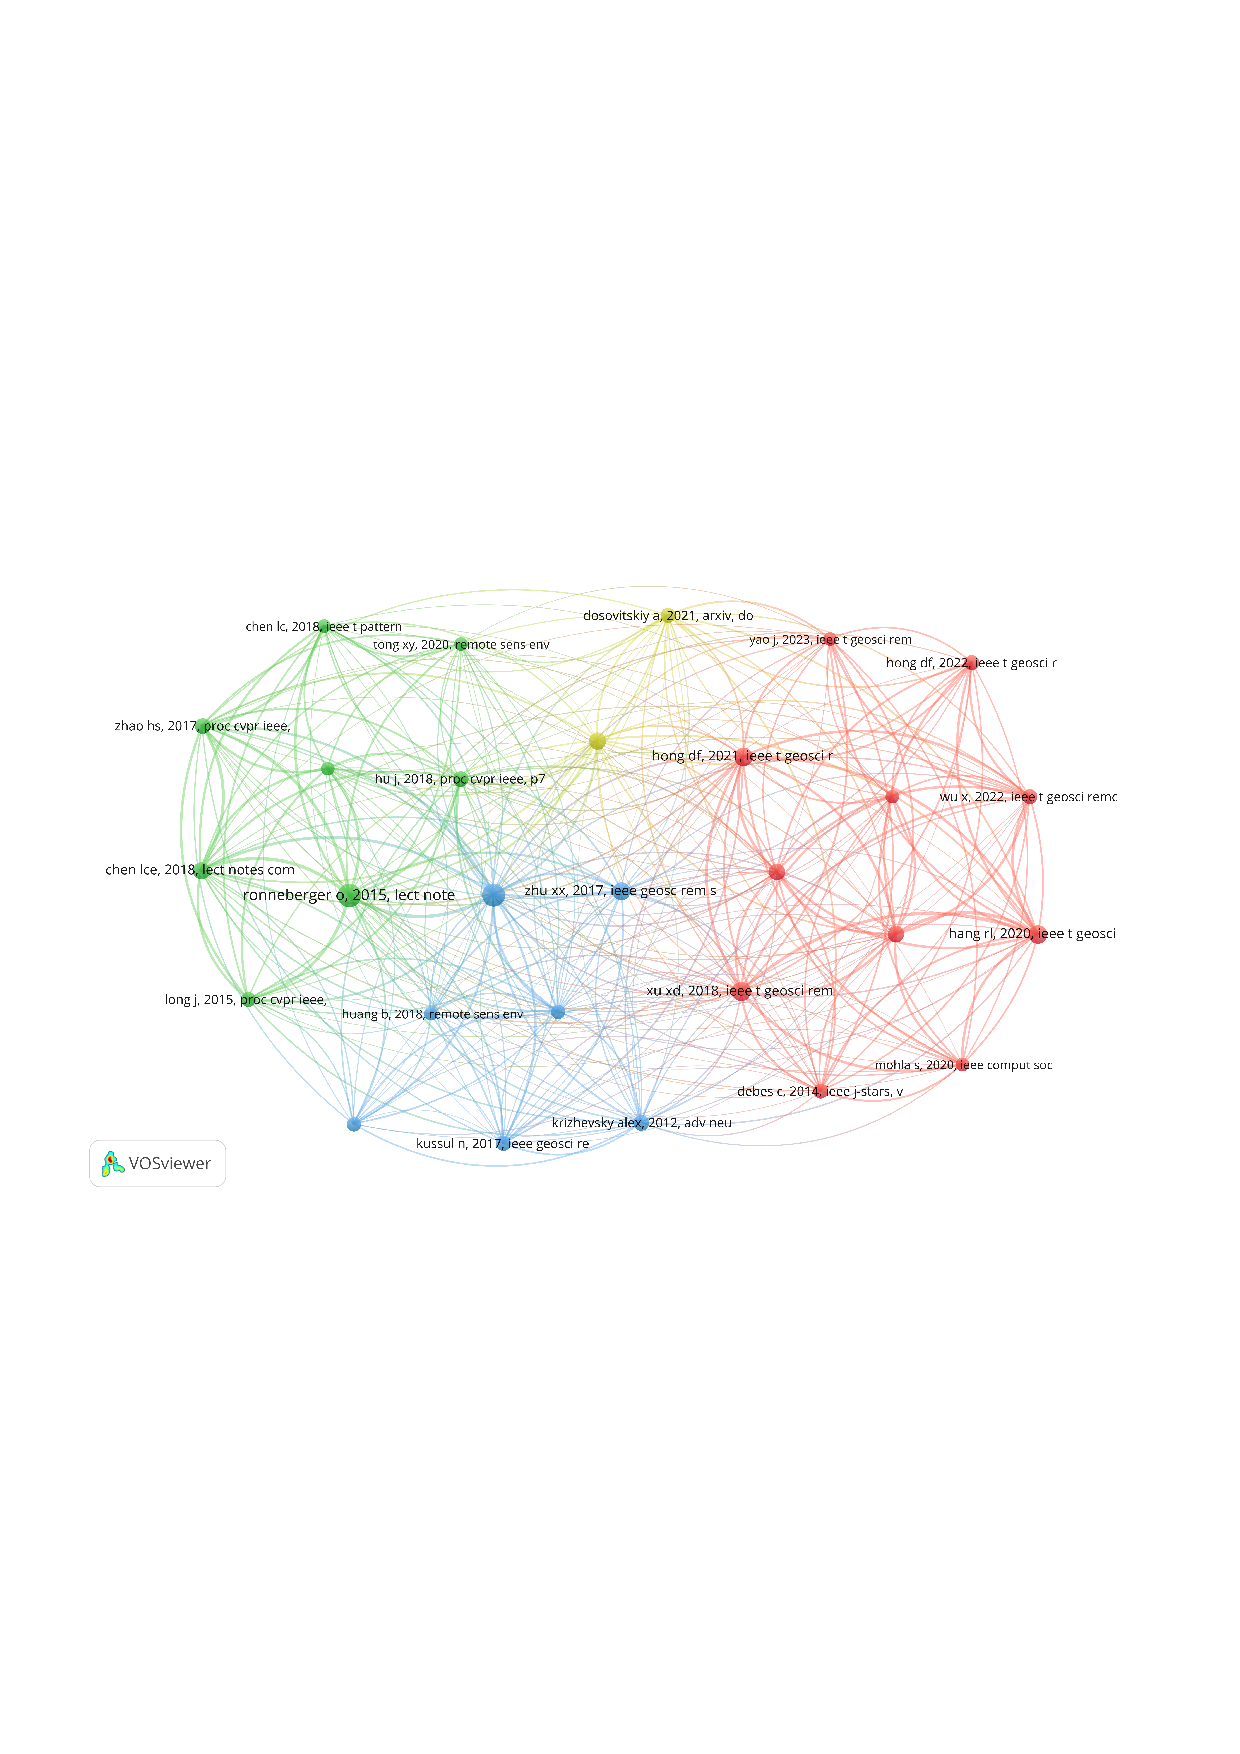
\includegraphics[width=0.98\linewidth]{Figures/picture_9.pdf}
	\caption{Document co-citation network revealing the intellectual structure of \DIFadd{the} \DIFadd{retrieved} LULC \DIFdel{research} \DIFadd{classification} \DIFadd{literature}\DIFadd{.} \DIFadd{Node} \DIFadd{size} \DIFadd{indicates} \DIFadd{citation} \DIFadd{prominence} \DIFadd{within} \DIFadd{the} \DIFadd{analysed} \DIFadd{network}\DIFadd{,} \DIFadd{colours} \DIFadd{indicate} \DIFadd{clusters}\DIFadd{,} \DIFadd{and} \DIFadd{links} \DIFadd{indicate} \DIFadd{co-citation} \DIFadd{relations}\DIFadd{.} \DIFadd{For} \DIFadd{readability}\DIFadd{,} \DIFadd{labels} \DIFadd{are} \DIFadd{displayed} \DIFadd{only} \DIFadd{for} \DIFadd{the} \DIFadd{more} \DIFadd{prominent} \DIFadd{nodes}\DIFadd{;} \DIFadd{all} \DIFadd{retained} \DIFadd{nodes} \DIFadd{contribute} \DIFadd{to} \DIFadd{network} \DIFadd{construction}.}
	\label{fig:intellectual_structure}
\end{figure}

\begin{enumerate}
	\item \textbf{Deep Learning Fundamentals (Blue Cluster):} This cluster represents the cornerstone of computer vision algorithms. Core nodes include Krizhevsky et al. (2012, AlexNet) and Simonyan \DIFdel{et} \DIFdel{al}\DIFdel{.} \DIFadd{and} \DIFadd{Zisserman} (2015, VGG) \citep{31, 32}. These landmark studies introduced the AlexNet architecture and VGG network, respectively. Although originating from general computer vision, they provided the foundational CNN architectures that serve as primary feature extractors for remote sensing imagery. The \DIFdel{highly} \DIFdel{cited} work by Marmanis et al. (2016) directly bridges this cluster with remote sensing, marking the successful transfer of ImageNet pre-trained models to Earth observation tasks.
	
	\item \textbf{Semantic Segmentation Paradigm (Green Cluster):} This cluster focuses on ``pixel-to-pixel'' classification methods, which are critical for LULC mapping. Key nodes include Long et al. (2015, FCN) {\hypersetup{citecolor=red}\color{red}\citep{ORIG33} } {\color{blue}\citep{33} }and Ronneberger et al. (2015, U-Net) \citep{34}. These studies established the ``encoder-decoder'' architecture, enabling end-to-end dense prediction. In the context of LULC, \DIFdel{this} \DIFdel{paradigm} \DIFdel{shifted} \DIFdel{the} \DIFdel{research} \DIFdel{focus} \DIFdel{from} \DIFadd{these} \DIFadd{methods} \DIFadd{support} \DIFadd{dense} \DIFadd{prediction} \DIFadd{and} \DIFadd{boundary} \DIFadd{delineation} \DIFadd{alongside} patch-based classification \DIFdel{to} \DIFdel{precise} \DIFdel{boundary} \DIFdel{delineation}.
	
	\item \textbf{Multi-source Data Fusion (Red Cluster):} \DIFdel{Dominated} \DIFadd{Including} \DIFadd{studies} by \DIFdel{scholars} \DIFdel{such} \DIFdel{as} Ghamisi P., Zhu X.X., and Hong D.F., this cluster represents the specific application of deep learning to heterogeneous remote sensing data. \DIFdel{This} \DIFdel{lineage} \DIFdel{originates} \DIFdel{from} \DIFdel{classical} \DIFdel{statistical} \DIFdel{modeling} \DIFdel{of} \DIFdel{sensor} \DIFdel{physics} \DIFdel{and} \DIFdel{the} \DIFdel{establishment} \DIFdel{of} \DIFdel{rigorous} \DIFdel{evaluation} \DIFdel{frameworks} \DIFdel{for} \DIFdel{pixel-level} \DIFdel{fusion} {\hypersetup{citecolor=red}\color{red}\citep{ORIG58}}\DIFdel{.} Unlike the general-algorithm clusters, this group specifically addresses fusion challenges involving hyperspectral \DIFadd{imagery} (HSI), LiDAR, and SAR data. The dense connections within this cluster highlight the intensive academic efforts in developing \DIFdel{specialized} \DIFadd{specialised} fusion modules to handle the unique physical attributes of remote sensing data.
	
	\item \textbf{Emerging Transformer Frontier (Yellow Cluster):} \DIFdel{Representing} \DIFdel{the} \DIFdel{latest} \DIFdel{paradigm} \DIFdel{shift}\DIFdel{,} This cluster \DIFdel{centers} \DIFadd{centres} on Dosovitskiy et al. (2021, Vision Transformer) \citep{35}. \DIFdel{It} \DIFdel{marks} \DIFdel{the} \DIFdel{transition} \DIFdel{from} \DIFdel{local} \DIFdel{convolutional} \DIFdel{operations} \DIFdel{to} \DIFdel{global} \DIFdel{attention} \DIFdel{mechanisms} \DIFadd{This} \DIFadd{work} \DIFadd{uses} \DIFadd{self-attention} \DIFadd{for} \DIFadd{interactions} \DIFadd{between} \DIFadd{image} \DIFadd{tokens}. The emergence of this cluster echoes \DIFdel{recent} \DIFdel{high-impact} papers such as Yao et al. (2023, ExViT), \DIFdel{indicating} \DIFdel{that} \DIFdel{the} \DIFdel{field} \DIFdel{is} \DIFdel{actively} \DIFdel{moving} \DIFdel{toward} \DIFdel{an} \DIFdel{era} \DIFdel{of} \DIFadd{reflecting} \DIFadd{interest} \DIFadd{in} \DIFadd{long-range} \DIFadd{spatial} \DIFadd{modelling} \DIFadd{rather} \DIFadd{than} \DIFadd{demonstrating} \DIFadd{a} \DIFadd{transition} \DIFadd{to} foundation models \DIFdel{capable} \DIFdel{of} \DIFdel{long-range} \DIFdel{spatial} \DIFdel{modeling} \DIFdel{of} \DIFdel{complex} \DIFdel{earth} \DIFdel{surfaces} \citep{36}.
\end{enumerate}

\subsection{Analysis of Emerging Research Methods}
Prior to the \DIFdel{dominance} \DIFadd{widespread} \DIFadd{use} of deep learning \DIFadd{in} \DIFadd{the} \DIFadd{literature} \DIFadd{reviewed} \DIFadd{here}, LULC research primarily relied on traditional machine learning algorithms and object-based analysis. As \DIFdel{summarized} \DIFadd{summarised} in Table~\ref{tab:traditional_methods}, SVM and RF have long been considered benchmark methods \DIFdel{due} \DIFdel{to} \DIFdel{their} \DIFdel{robustness} \DIFdel{with} \DIFdel{small} \DIFdel{samples} \DIFadd{for} \DIFadd{small-sample} and high-dimensional \DIFdel{data} \DIFadd{tasks}\DIFadd{,} \DIFadd{with} \DIFadd{performance} \DIFadd{depending} \DIFadd{on} \DIFadd{features} \DIFadd{and} \DIFadd{tuning}.

\begin{table}[!htbp]
	\centering
	\setlength{\belowcaptionskip}{5pt} 
	\caption{Traditional methods in LULC research.} 
		\label{tab:traditional_methods}
		\small 
		\setlength{\tabcolsep}{3pt}
		\renewcommand{\arraystretch}{1.4} 
		\begin{tabular}{@{} p{2.0cm} p{5.2cm} p{6.2cm} @{}} 
		\toprule
		\textbf{Method} & \textbf{Advantages} & \textbf{LULC Application Scenarios} \\ 
		\midrule
		SVM & \DIFadd{Can} \DIFadd{achieve} strong \DIFdel{generalization} \DIFadd{generalisation} with small samples. & \DIFdel{Fine-classification} \DIFadd{Fine-grained} \DIFadd{classification} with hyperspectral data. \\ \addlinespace[3pt]
		RF  & \DIFadd{Can} \DIFadd{achieve} high accuracy and stability; \DIFdel{resists} \DIFadd{can} \DIFadd{resist} overfitting. & Large-scale mapping on cloud platforms like \DIFadd{Google} \DIFadd{Earth} \DIFadd{Engine} \DIFadd{(}GEE\DIFadd{)}. \\ \addlinespace[3pt]
		\DIFadd{Artificial} \DIFadd{neural} \DIFadd{network} \DIFadd{(}ANN\DIFadd{)} & \DIFdel{Handles} \DIFadd{Can} \DIFadd{handle} non-linear relationships effectively. & \DIFadd{Classification} \DIFadd{of} \DIFadd{very} \DIFadd{high} \DIFadd{resolution} \DIFadd{(}VHR\DIFadd{)} imagery \DIFdel{to} \DIFdel{reduce} \DIFdel{pixel} \DIFdel{fragmentation}. \\ 
		\bottomrule
	\end{tabular}
\end{table}

\DIFadd{The} \DIFadd{archived} \DIFadd{second-stage} \DIFadd{content} \DIFadd{coding} \DIFadd{contains} \DIFadd{163} \DIFadd{records} \DIFadd{with} \DIFadd{an} \DIFadd{explicit} \DIFadd{and} \DIFadd{classifiable} \DIFadd{fusion} \DIFadd{operation}\DIFadd{.} \DIFadd{Among} \DIFadd{these} \DIFadd{records}\DIFadd{,} \DIFadd{131} \DIFadd{were} \DIFadd{assigned} to \DIFdel{further} \DIFdel{quantify} \DIFadd{feature-level-only} \DIFadd{fusion}\DIFadd{,} \DIFadd{18} \DIFadd{to} \DIFadd{hybrid} \DIFadd{fusion} \DIFadd{(}\DIFadd{12} \DIFadd{data--feature} \DIFadd{and} \DIFadd{six} \DIFadd{feature--decision} \DIFadd{combinations}\DIFadd{)}\DIFadd{,} \DIFadd{seven} \DIFadd{to} \DIFadd{data-level-only} \DIFadd{fusion}\DIFadd{,} \DIFadd{and} \DIFadd{seven} \DIFadd{to} \DIFadd{decision-level-only} \DIFadd{fusion}\DIFadd{.} \DIFadd{These} \DIFadd{counts} \DIFadd{describe} the \DIFdel{shift} \DIFdel{toward} \DIFdel{modern} \DIFdel{architectures}\DIFdel{,} \DIFdel{we} \DIFdel{analyzed} \DIFadd{criterion-defined} \DIFadd{fusion-level} \DIFadd{subset} \DIFadd{rather} \DIFadd{than} the distribution of \DIFdel{methodological} \DIFdel{approaches} \DIFdel{within} \DIFadd{fusion} \DIFadd{levels} \DIFadd{in} \DIFadd{all} \DIFadd{261} \DIFadd{bibliometric} \DIFadd{records}\DIFadd{.} The \DIFdel{sampled} \DIFdel{literature}\DIFdel{.} \DIFdel{Here}\DIFdel{,} \DIFdel{feature-level} \DIFdel{fusion} \DIFdel{has} \DIFdel{emerged} \DIFdel{as} \DIFdel{the} \DIFdel{absolute} \DIFdel{dominant} \DIFdel{paradigm}\DIFdel{,} \DIFdel{accounting} \DIFdel{for} \DIFdel{80}\DIFdel{.}\DIFdel{9} \DIFdel{of} \DIFdel{the} \DIFdel{studies}\DIFdel{.} \DIFdel{This} \DIFdel{is} \DIFdel{followed} \DIFdel{by} \DIFdel{hybrid} \DIFdel{Data}\DIFdel{+}\DIFdel{Feature} \DIFdel{fusion} \DIFdel{(}\DIFdel{7}\DIFdel{.}\DIFdel{4}\DIFdel{)} \DIFdel{and} \DIFdel{decision-level} \DIFdel{fusion} \DIFdel{(}\DIFdel{4}\DIFdel{.}\DIFdel{3}\DIFdel{)}\DIFdel{.} \DIFdel{This} \DIFdel{distribution} \DIFdel{underlines} \DIFdel{a} \DIFdel{significant} \DIFdel{shift} \DIFadd{other} \DIFadd{98} \DIFadd{records} \DIFadd{remained} in the \DIFdel{research} \DIFdel{community} \DIFdel{towards} \DIFdel{integrating} \DIFdel{high-level} \DIFdel{semantic} \DIFdel{features} \DIFdel{rather} \DIFdel{than} \DIFdel{relying} \DIFdel{on} \DIFdel{raw} \DIFdel{signal} \DIFdel{concatenation} \DIFadd{bibliometric} \DIFadd{corpus} \DIFadd{but} \DIFadd{were} \DIFadd{excluded} \DIFadd{from} \DIFadd{fusion-level} \DIFadd{counts}\DIFadd{,} \DIFadd{as} \DIFadd{described} \DIFadd{in} \DIFadd{Section}\DIFadd{~}{\color{blue}\ref{sec:fusion_coding}}. The \DIFdel{prevalence} \DIFadd{counts} \DIFadd{are} \DIFadd{not} \DIFadd{used} \DIFadd{to} \DIFadd{support} \DIFadd{field-level} \DIFadd{claims} \DIFadd{about} \DIFadd{the} \DIFadd{superiority} \DIFadd{or} \DIFadd{dominance} of \DIFdel{feature-level} \DIFadd{any} fusion \DIFdel{is} \DIFdel{deeply} \DIFdel{rooted} \DIFdel{in} \DIFdel{the} \DIFdel{surge} \DIFdel{of} \DIFdel{deep} \DIFdel{learning} \DIFdel{techniques} \DIFadd{level}.


As shown in the keyword density \DIFdel{visualization} \DIFadd{visualisation} (Fig.~\ref{fig:keyword_density}), the \DIFdel{absolute} \DIFdel{`}\DIFdel{`}\DIFdel{gravitational} \DIFdel{centers''} \DIFdel{of} \DIFadd{highest-density} \DIFadd{regions} \DIFadd{in} the \DIFdel{field} \DIFadd{retrieved} \DIFadd{corpus} are concentrated around ``deep learning'', ``fusion'', and ``CNN''. These nodes \DIFdel{form} \DIFdel{the} \DIFdel{core} \DIFdel{technological} \DIFdel{drivers}\DIFdel{,} \DIFdel{where} \DIFdel{multi-scale} \DIFadd{reflect} \DIFadd{attention} \DIFadd{to} \DIFadd{neural} feature extraction \DIFdel{through} \DIFdel{CNN} \DIFdel{has} \DIFdel{become} \DIFdel{the} \DIFdel{standard} \DIFdel{implementation} \DIFdel{for} \DIFdel{achieving} \DIFdel{the} \DIFdel{high-level} \DIFdel{semantic} \DIFdel{integration} \DIFdel{mentioned} \DIFadd{and} \DIFadd{fusion}. \DIFdel{Notably}\DIFdel{,} \DIFdel{while} Traditional methods like SVM appear as lower-density peripheral nodes, \DIFdel{the} \DIFdel{intense} \DIFdel{yellow} \DIFdel{clusters} \DIFdel{signify} \DIFdel{that} \DIFdel{the} \DIFdel{field} \DIFdel{has} \DIFdel{fully} \DIFdel{entered} \DIFdel{an} \DIFdel{era} \DIFdel{dominated} \DIFdel{by} \DIFdel{neural-based} \DIFdel{feature} \DIFadd{but} \DIFadd{this} \DIFadd{distribution} \DIFadd{is} \DIFadd{conditioned} \DIFadd{on} \DIFadd{a} \DIFadd{search} \DIFadd{requiring} \DIFadd{deep} \DIFadd{learning} \DIFadd{and} fusion \DIFadd{terms}\DIFadd{;} \DIFadd{it} \DIFadd{cannot} \DIFadd{establish} \DIFadd{their} \DIFadd{relative} \DIFadd{prevalence} \DIFadd{across} \DIFadd{LULC} \DIFadd{research}.

\begin{figure}[!htbp]
	\centering
	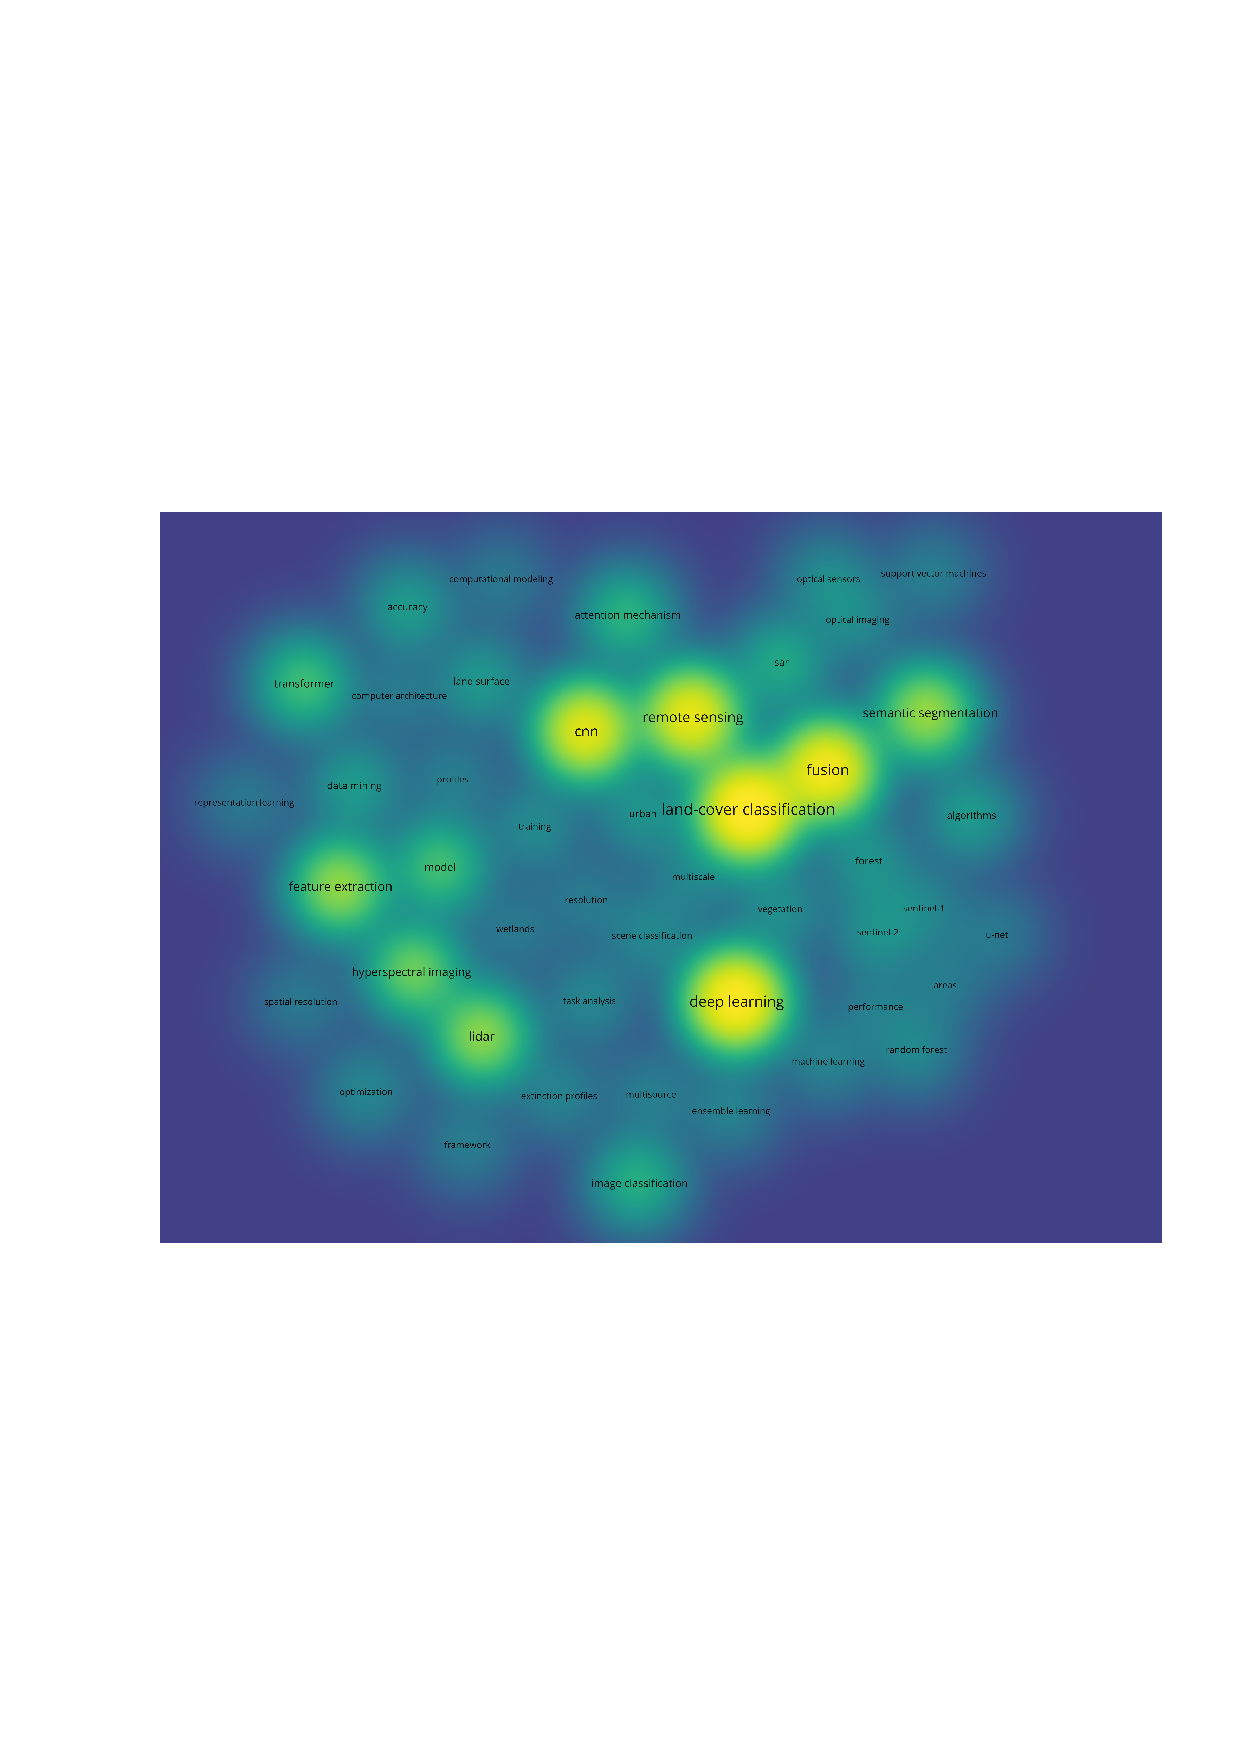
\includegraphics[width=1.0\columnwidth]{Figures/new_Relitu.pdf}
	\caption{Density \DIFdel{visualization} \DIFadd{visualisation} of keyword hotspots\DIFdel{,} \DIFdel{identifying} \DIFadd{in} the \DIFdel{core} \DIFdel{technological} \DIFdel{drivers} \DIFdel{within} \DIFdel{the} \DIFadd{retrieved} LULC \DIFdel{simulation} \DIFdel{domain} \DIFadd{classification} \DIFadd{literature}.}
	\label{fig:keyword_density}
\end{figure}

Currently, the \DIFdel{maturation} \DIFadd{evaluation} of these deep learning fusion models \DIFdel{is} \DIFadd{relies} heavily \DIFdel{based} on \DIFdel{robust} \DIFdel{validation} \DIFdel{through} benchmark datasets. The high-density focus on ``hyperspectral imaging'' and ``LiDAR'' in Fig.~\ref{fig:keyword_density} is directly reflected in the dataset \DIFdel{utilization} \DIFadd{utilisation} rankings. Our analysis (Fig.~\ref{fig:datasets_ranking}) reveals that Houston (25 studies) and Trento (15 studies) \DIFdel{remain} \DIFadd{were} the most prevalent benchmarks \DIFadd{in} \DIFadd{the} \DIFadd{included} \DIFadd{corpus}. This concentration highlights the community's reliance on \DIFdel{standardized} \DIFadd{standardised}, multi-modal data to evaluate the performance of feature-fusion architectures in complex urban and agricultural environments. \DIFadd{However}\DIFadd{,} \DIFadd{concentration} \DIFadd{on} \DIFadd{a} \DIFadd{few} \DIFadd{curated} \DIFadd{datasets} \DIFadd{limits} \DIFadd{conclusions} \DIFadd{about} \DIFadd{cross-region}\DIFadd{,} \DIFadd{large-area}\DIFadd{,} \DIFadd{and} \DIFadd{temporally} \DIFadd{dynamic} \DIFadd{mapping}\DIFadd{.}

\begin{figure}[!htbp]
	\centering
	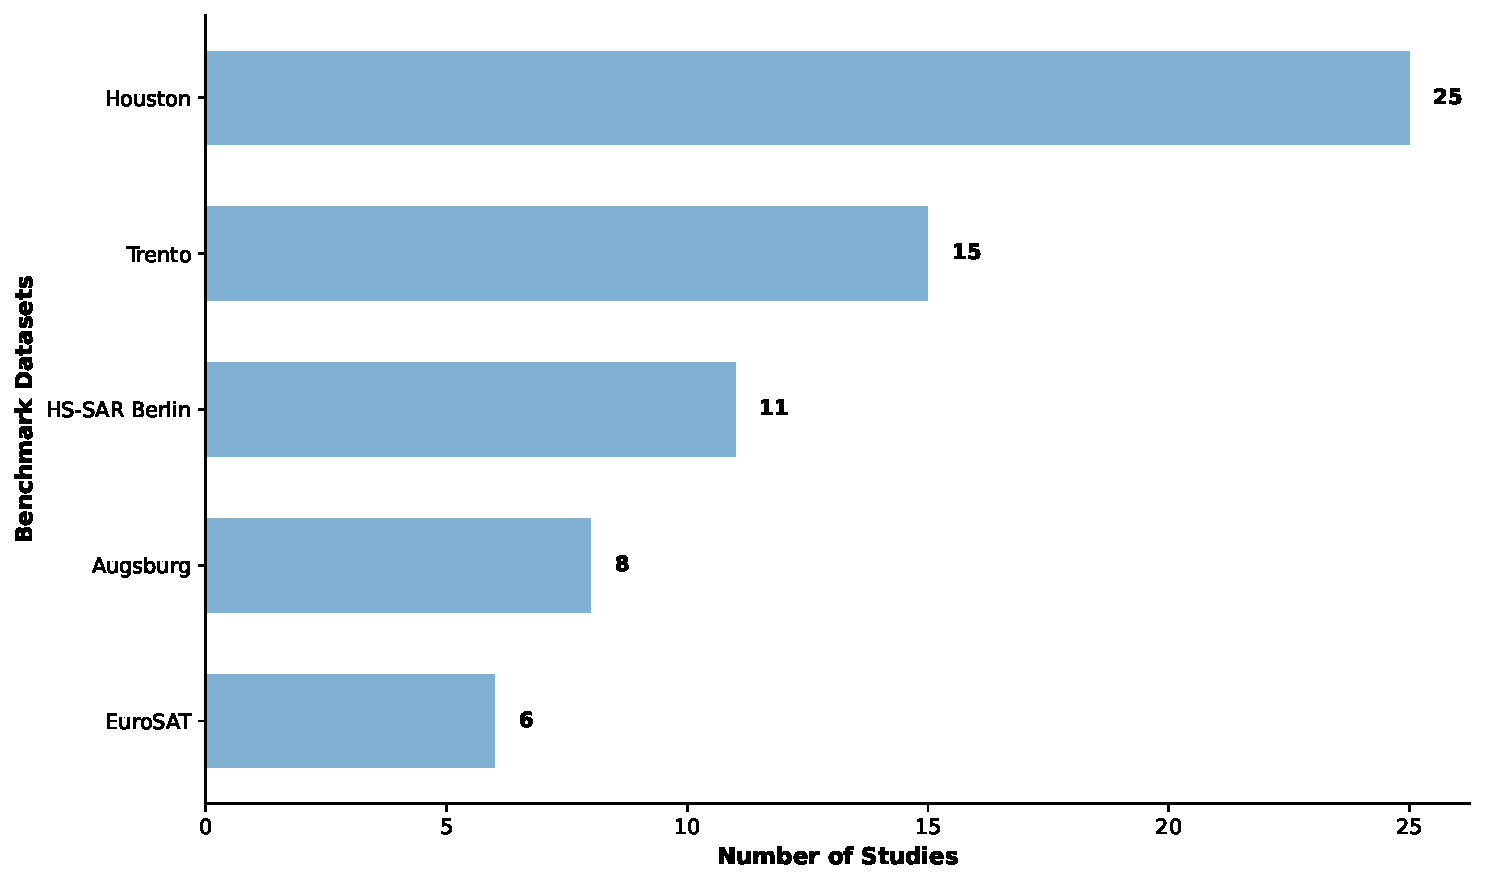
\includegraphics[width=1.0\columnwidth]{Figures/top_datasets_ranking.pdf}
	\caption{Frequency of \DIFdel{benchmark} datasets \DIFdel{utilized} \DIFadd{utilised} in the \DIFdel{analyzed} \DIFadd{analysed} LULC fusion studies. \DIFadd{EuroSAT} \DIFadd{is} \DIFadd{shown} \DIFadd{as} \DIFadd{a} \DIFadd{corpus-frequency} \DIFadd{observation}\DIFadd{;} \DIFadd{because} \DIFadd{it} \DIFadd{contains} \DIFadd{Sentinel-2} \DIFadd{multispectral} \DIFadd{imagery} \DIFadd{rather} \DIFadd{than} \DIFadd{multimodal} \DIFadd{data}\DIFadd{,} \DIFadd{it} \DIFadd{is} \DIFadd{not} \DIFadd{included} \DIFadd{in} \DIFadd{Table}\DIFadd{~}{\color{blue}\ref{tab:datasets_detail}}\DIFadd{.}}
	\label{fig:datasets_ranking}
\end{figure}

\begin{table}[!htbp]
	\centering
	\setlength{\belowcaptionskip}{8pt}
	\caption{Technical specifications of \DIFdel{the} \DIFdel{five} \DIFdel{most} \DIFdel{utilized} \DIFadd{representative} \DIFadd{multimodal} benchmark datasets \DIFadd{used} in LULC \DIFdel{fusion} \DIFdel{research} \DIFadd{classification}.}
	\label{tab:datasets_detail}
	\scriptsize
	\setlength{\tabcolsep}{3pt}
	\renewcommand{\arraystretch}{1.25}
	\begin{tabular}{@{} p{1.8cm} p{3.5cm} p{3.2cm} c p{3.5cm} @{}}
		\toprule
		\textbf{Dataset} & \textbf{Modalities (Sensors)} & \textbf{Resolution} & \textbf{Classes} & \textbf{Dimensions (px)} \\ 
		\midrule
Houston 2013 & HSI (144 bands) + LiDAR & 2.5 m & 15 & $349 \times 1905$ \\
Trento & HSI (\DIFdel{6}\hspace{0.33em}\DIFadd{63} bands) + LiDAR & 1.0 m & 6 & $600 \times 166$ \\
\textcolor{DIFdelcolor}{HS-SAR Berlin} & \textcolor{DIFdelcolor}{HSI + SAR (dual-pol)} & \textcolor{DIFdelcolor}{3.5 m} & \textcolor{DIFdelcolor}{8} & \textcolor{DIFdelcolor}{$1623 \times 1076$} \\
\textcolor{DIFaddcolor}{Berlin} & \textcolor{DIFaddcolor}{HSI (244 bands) + SAR} & \textcolor{DIFaddcolor}{30 m (HSI); 13--13.9 m (SAR)} & \textcolor{DIFaddcolor}{8} & \textcolor{DIFaddcolor}{$797 \times 220$ (HSI); $1723 \times 476$ (SAR)} \\
\textcolor{DIFdelcolor}{Augsburg} & \textcolor{DIFdelcolor}{SAR + HSI + DSM} & \textcolor{DIFdelcolor}{30m / 1m} & \textcolor{DIFdelcolor}{7} & \textcolor{DIFdelcolor}{$1528 \times 918$} \\
\textcolor{DIFaddcolor}{Augsburg} & \textcolor{DIFaddcolor}{HSI (180 bands) + SAR + digital surface model (DSM)} & \textcolor{DIFaddcolor}{30 m (co-registered products)} & \textcolor{DIFaddcolor}{7} & \textcolor{DIFaddcolor}{$332 \times 485$} \\
\textcolor{DIFdelcolor}{EuroSAT} & \textcolor{DIFdelcolor}{Multispectral (Sentinel-2)} & \textcolor{DIFdelcolor}{10 m} & \textcolor{DIFdelcolor}{10} & \textcolor{DIFdelcolor}{$64 \times 64$ (per patch)} \\
\textcolor{DIFaddcolor}{MUUFL Gulfport} & \textcolor{DIFaddcolor}{HSI (64 bands) + LiDAR} & \textcolor{DIFaddcolor}{1 m (co-registered grid)} & \textcolor{DIFaddcolor}{11} & \textcolor{DIFaddcolor}{$325 \times 220$} \\
\bottomrule
	\end{tabular}
\end{table}

As evidenced by the technical specifications in Table~\ref{tab:datasets_detail}, the integration of heterogeneous data requires different algorithmic strategies. The diversity in spatial resolution and spectral dimensionality across these benchmarks, particularly the HSI and LiDAR combinations in Houston and MUUFL \DIFadd{Gulfport}, has historically driven the evolution of fusion methodologies.  \DIFadd{EuroSAT} \DIFadd{is} \DIFadd{retained} \DIFadd{in} \DIFadd{Fig}\DIFadd{.}\DIFadd{~}{\color{blue}\ref{fig:datasets_ranking} }\DIFadd{only} \DIFadd{as} \DIFadd{a} \DIFadd{corpus-frequency} \DIFadd{observation} \DIFadd{and} \DIFadd{is} \DIFadd{excluded} \DIFadd{from} \DIFadd{Table}\DIFadd{~}{\color{blue}\ref{tab:datasets_detail} }\DIFadd{because} \DIFadd{it} \DIFadd{contains} \DIFadd{Sentinel-2} \DIFadd{multispectral} \DIFadd{imagery} \DIFadd{rather} \DIFadd{than} \DIFadd{multimodal} \DIFadd{observations}\DIFadd{.} \DIFadd{Trento}\DIFadd{,} \DIFadd{Berlin}\DIFadd{,} \DIFadd{Augsburg}\DIFadd{,} \DIFadd{and} \DIFadd{MUUFL} \DIFadd{specifications} \DIFadd{follow} \DIFadd{published} \DIFadd{benchmark} \DIFadd{descriptions} \DIFadd{and} \DIFadd{the} \DIFadd{official} \DIFadd{release} {\color{blue}\citep{duan2020multilevel,hong2021benchmarks,gader2013muufl,zare2018muufl}}\DIFadd{.}

Driven by this evidence, research typically \DIFdel{categorizes} \DIFadd{categorises} fusion technologies into three \DIFdel{progressive} \DIFdel{stages} \DIFadd{levels}: Data-level Fusion, Feature-level Fusion, and Decision-level Fusion, as illustrated in Fig.~\ref{fig:fusion_stages}. \DIFdel{The} \DIFdel{robust} \DIFdel{data} \DIFdel{structures} \DIFdel{provided} \DIFdel{by} These \DIFdel{benchmarks} \DIFdel{have} \DIFdel{specifically} \DIFdel{catalyzed} \DIFdel{the} \DIFdel{shift} \DIFdel{toward} \DIFdel{feature-level} \DIFadd{are} \DIFadd{alternative} \DIFadd{integration} \DIFadd{choices} \DIFadd{rather} \DIFadd{than} \DIFadd{a} \DIFadd{mandatory} \DIFadd{progression}\DIFadd{.} \DIFadd{Hybrid} fusion\DIFdel{,} \DIFdel{which} \DIFdel{uses} \DIFdel{deep} \DIFdel{learning} \DIFdel{to} \DIFdel{align} \DIFdel{complex} \DIFdel{semantic} \DIFdel{representations} \DIFdel{from} \DIFdel{different} \DIFdel{sensors} \DIFadd{combines} \DIFadd{explicit} \DIFadd{integration} \DIFadd{at} \DIFadd{two} \DIFadd{or} \DIFadd{more} \DIFadd{levels}.

\begin{figure}[!htbp]
	\centering
	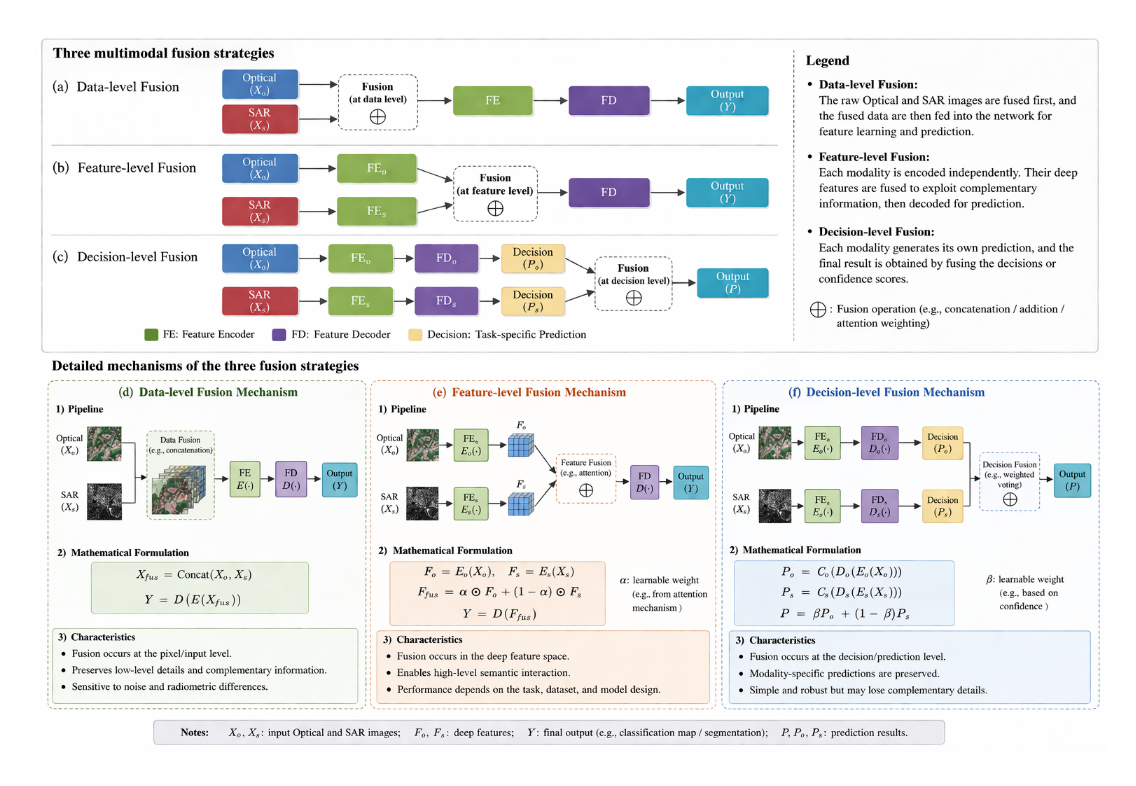
\includegraphics[width=1.0\columnwidth, trim=0 10 0 10, clip]{Figures/Fusion_Picture.pdf}
	\caption{Three \DIFdel{stages} \DIFdel{of} \DIFadd{principal} fusion \DIFdel{technology} \DIFadd{levels} \DIFadd{considered} in LULC \DIFadd{classification}: (a) data-level fusion, (b) feature-level fusion, and (c) decision-level fusion. \DIFadd{These} \DIFadd{levels} \DIFadd{represent} \DIFadd{alternative} \DIFadd{design} \DIFadd{choices} \DIFadd{rather} \DIFadd{than} \DIFadd{a} \DIFadd{mandatory} \DIFadd{progression}\DIFadd{.}}
	\label{fig:fusion_stages}
\end{figure}

\DIFadd{Table}\DIFadd{~}{\color{blue}\ref{tab:fusion_levels} }\DIFadd{compares} \DIFadd{the} \DIFadd{main} \DIFadd{design} \DIFadd{and} \DIFadd{evaluation} \DIFadd{implications} \DIFadd{of} \DIFadd{the} \DIFadd{four} \DIFadd{fusion} \DIFadd{levels}\DIFadd{.} \DIFadd{Fusion} \DIFadd{level} \DIFadd{is} \DIFadd{defined} \DIFadd{by} \DIFadd{the} \DIFadd{first} \DIFadd{stage} \DIFadd{at} \DIFadd{which} \DIFadd{modality-specific} \DIFadd{streams} \DIFadd{exchange} \DIFadd{information}\DIFadd{;} \DIFadd{hybrid} \DIFadd{fusion} \DIFadd{requires} \DIFadd{explicit} \DIFadd{fusion} \DIFadd{at} \DIFadd{two} \DIFadd{or} \DIFadd{more} \DIFadd{distinct} \DIFadd{stages}\DIFadd{.} \DIFadd{Representative} \DIFadd{implementations} \DIFadd{for} \DIFadd{each} \DIFadd{level} \DIFadd{are} \DIFadd{identified} \DIFadd{in} \DIFadd{the} \DIFadd{table} \DIFadd{note}\DIFadd{.} \DIFadd{Here} {\color{blue}$M$} \DIFadd{is} \DIFadd{the} \DIFadd{number} \DIFadd{of} \DIFadd{modalities}\DIFadd{,} {\color{blue}$C$} \DIFadd{the} \DIFadd{number} \DIFadd{of} \DIFadd{classes}\DIFadd{,} {\color{blue}$d_m$} \DIFadd{the} \DIFadd{input} \DIFadd{width} \DIFadd{of} \DIFadd{modality} {\color{blue}$m$}\DIFadd{,} {\color{blue}$N_i$} \DIFadd{and} {\color{blue}$N_j$} \DIFadd{the} \DIFadd{numbers} \DIFadd{of} \DIFadd{positions} \DIFadd{or} \DIFadd{tokens}\DIFadd{,} \DIFadd{and} {\color{blue}$d$} \DIFadd{the} \DIFadd{latent} \DIFadd{dimension}\DIFadd{.} \DIFadd{The} \DIFadd{complexity} \DIFadd{terms} \DIFadd{describe} \DIFadd{representative} \DIFadd{operators} \DIFadd{rather} \DIFadd{than} \DIFadd{complete} \DIFadd{implementations}\DIFadd{.} \DIFadd{Accuracy} \DIFadd{and} \DIFadd{measured} \DIFadd{runtime} \DIFadd{are} \DIFadd{not} \DIFadd{ranked} \DIFadd{across} \DIFadd{publications} \DIFadd{because} \DIFadd{datasets}\DIFadd{,} \DIFadd{hardware}\DIFadd{,} \DIFadd{training} \DIFadd{budgets}\DIFadd{,} \DIFadd{and} \DIFadd{evaluation} \DIFadd{protocols} \DIFadd{differ}\DIFadd{.}

\begin{table}[!htbp]
	\centering
	\color{DIFaddcolor}
	\caption{Design and evaluation considerations for multimodal LULC fusion levels.}
	\label{tab:fusion_levels}
	\footnotesize
	\setlength{\tabcolsep}{2pt}
	\renewcommand{\arraystretch}{1.18}
	\begin{tabular}{@{} >{\raggedright\arraybackslash}p{1.25cm} >{\raggedright\arraybackslash}p{2.90cm} >{\raggedright\arraybackslash}p{3.00cm} >{\raggedright\arraybackslash}p{2.65cm} >{\raggedright\arraybackslash}p{3.65cm} @{}}
		\toprule
		\textbf{Fusion level} & \textbf{Integration and data needs} & \textbf{Training and computation} & \textbf{Key risks} & \textbf{Minimum evidence and suitable conditions} \\
		\midrule
		Data-level & Combines co-registered inputs before representation learning. Grid concatenation requires spatial correspondence and sensor-appropriate normalisation. & Usually trained jointly. Concatenation increases encoder input width to $\sum_m d_m$; cost grows with source count and preprocessing. & Misregistration, acquisition-time mismatch, redundant or noisy bands, and dominance of a high-dimensional source. & Compare each source with concatenation and perturb registration and acquisition time. Most suitable when inputs are accurately aligned and low-level correspondence is important. \\
		\addlinespace[2pt]
		Feature-level & Combines intermediate modality-specific or shared representations. Resampling or learned alignment can accommodate some resolution differences, but semantic correspondence remains necessary. & Uses separate encoders and a fusion module. Dense pairwise cross-attention scales as $O(N_iN_jd)$ in time and $O(N_iN_j)$ in attention memory \citep{vaswani2017attention}. & Modality dominance, overfitting, alignment shift, and brittleness to missing or corrupted sources. & Require modality ablation, missing- and misaligned-source stress tests, and a compute-matched late-fusion baseline. Suitable when detailed cross-modal interaction is required. \\
		\addlinespace[2pt]
		Decision-level & Aggregates scores, probabilities, labels, or maps. Feature spaces need not match, but classes and spatial units must be compatible. & Branches may be trained independently. Simple score averaging adds $O(MC)$ operations beyond branch inference. & Miscalibration, correlated errors, incompatible taxonomies, and loss of fine cross-modal interaction. & Report branch performance, error correlation, calibration, and missing-branch tests. Suitable for ensembles and modular sensor pipelines. \\
		\addlinespace[2pt]
		Hybrid & Uses explicit fusion at two or more stages, such as feature interaction followed by score aggregation. & Architecture-dependent and jointly or sequentially trained. Report parameters, floating-point operations, memory, and latency. & Redundant paths, cross-stage co-adaptation, optimisation instability, error propagation, and unclear attribution of gains. & Require stage-wise ablation and compute-matched single-level baselines. Suitable when both fine cross-modal interaction and modular prediction are needed. \\
		\midrule
		\multicolumn{5}{@{}>{\raggedright\arraybackslash}p{13.45cm}@{}}{\scriptsize \textit{Note.} Representative implementations comprise data-level fusion \citep{6,37}, feature-level fusion \citep{23,41,zhang2023multimodal}, decision-level fusion \citep{55}, and hybrid feature--decision fusion \citep{hang2020coupled}. These references illustrate the respective fusion levels; the risks and minimum-evidence recommendations are the authors' synthesis and are not attributed in full to any individual study.} \\
		\bottomrule
	\end{tabular}
\end{table}

\DIFadd{The} \DIFadd{entries} \DIFadd{in} \DIFadd{Table}\DIFadd{~}{\color{blue}\ref{tab:fusion_levels} }\DIFadd{are} \DIFadd{conditional} \DIFadd{design} \DIFadd{expectations} \DIFadd{rather} \DIFadd{than} \DIFadd{universal} \DIFadd{rankings}\DIFadd{.} \DIFadd{The} \DIFadd{cited} \DIFadd{studies} \DIFadd{illustrate} \DIFadd{implementations} \DIFadd{of} \DIFadd{particular} \DIFadd{fusion} \DIFadd{levels} \DIFadd{but} \DIFadd{do} \DIFadd{not} \DIFadd{establish} \DIFadd{that} \DIFadd{one} \DIFadd{level} \DIFadd{is} \DIFadd{uniformly} \DIFadd{more} \DIFadd{accurate}\DIFadd{,} \DIFadd{efficient}\DIFadd{,} \DIFadd{robust}\DIFadd{,} \DIFadd{or} \DIFadd{interpretable}\DIFadd{.} \DIFadd{In} \DIFadd{hyperspectral} \DIFadd{classification}\DIFadd{,} \DIFadd{spatially} \DIFadd{overlapping} \DIFadd{sampling} \DIFadd{can} \DIFadd{inflate} \DIFadd{performance} \DIFadd{estimates} {\color{blue}\citep{liang2017sampling}}\DIFadd{;} \DIFadd{comparisons} \DIFadd{should} \DIFadd{therefore} \DIFadd{use} \DIFadd{identical} \DIFadd{preprocessing} \DIFadd{and} \DIFadd{geographically} \DIFadd{disjoint} \DIFadd{splits} \DIFadd{where} \DIFadd{possible}\DIFadd{.} \DIFadd{Temporal} \DIFadd{leakage}\DIFadd{,} \DIFadd{class} \DIFadd{imbalance}\DIFadd{,} \DIFadd{label} \DIFadd{uncertainty}\DIFadd{,} \DIFadd{and} \DIFadd{inconsistent} \DIFadd{preprocessing} \DIFadd{are} \DIFadd{likewise} \DIFadd{evaluation-wide} \DIFadd{threats}\DIFadd{.} \DIFadd{Comparative} \DIFadd{studies} \DIFadd{should} \DIFadd{include} \DIFadd{the} \DIFadd{strongest} \DIFadd{single-modality} \DIFadd{model}\DIFadd{,} \DIFadd{simple} \DIFadd{input} \DIFadd{concatenation}\DIFadd{,} \DIFadd{simple} \DIFadd{score} \DIFadd{averaging}\DIFadd{,} \DIFadd{and} \DIFadd{a} \DIFadd{parameter-} \DIFadd{or} \DIFadd{compute-matched} \DIFadd{baseline} \DIFadd{where} \DIFadd{applicable}\DIFadd{.}

\FloatBarrier

\subsection{\DIFadd{Data-Level} Fusion}
\DIFdel{Data}
\DIFadd{Data-level} fusion, often referred to as pixel-level or raw-level fusion, involves the direct integration of \DIFadd{co-registered} multimodal data sources, such as optical imagery, \DIFdel{LiDAR} \DIFdel{point} \DIFdel{clouds} \DIFadd{LiDAR-derived} \DIFadd{products}, and Synthetic Aperture Radar (SAR) \citep{57}. Bibliometric trends from 2016 to 2025 indicate that while keywords such as ``LiDAR'' and ``remote sensing'' \DIFdel{maintain} \DIFdel{significant} \DIFdel{research} \DIFdel{heat} \DIFadd{occur} \DIFadd{frequently} \DIFadd{in} \DIFadd{the} \DIFadd{retrieved} \DIFadd{corpus} \citep{38, 39}, \DIFdel{emerging} \DIFdel{focus} \DIFdel{has} \DIFdel{shifted} \DIFdel{toward} \DIFadd{studies} \DIFadd{investigate} the synergy of these sensors to \DIFdel{overcome} \DIFadd{address} individual spectral or structural limitations. The prominent status of LiDAR is attributed to its capacity to provide high-precision 3D coordinates and vegetation structure information, which \DIFdel{effectively} \DIFdel{compensates} \DIFdel{for} \DIFdel{the} \DIFdel{spectral} \DIFdel{saturation} \DIFdel{and} \DIFdel{cloud-cover} \DIFdel{vulnerabilities} \DIFdel{of} \DIFadd{can} \DIFadd{complement} optical \DIFadd{imagery} \DIFadd{from} sensors like Sentinel-2\DIFadd{;} \DIFadd{cloud-penetrating} \DIFadd{observations} \DIFadd{are} \DIFadd{provided} \DIFadd{by} \DIFadd{SAR} \DIFadd{rather} \DIFadd{than} \DIFadd{LiDAR} \citep{40}.

Despite its foundational importance, \DIFdel{data} \DIFadd{data-level} fusion faces persistent technical bottlenecks, particularly in multi-source spatial registration and heterogeneous noise suppression \citep{41}. \DIFdel{Our} \DIFdel{analysis} \DIFdel{suggests} \DIFdel{a} \DIFdel{paradigm} \DIFdel{shift} \DIFdel{in} \DIFadd{Statistical} \DIFadd{models} \DIFadd{of} \DIFadd{heterogeneous} \DIFadd{SAR} \DIFadd{returns} \DIFadd{illustrate} the \DIFdel{role} \DIFdel{of} \DIFdel{data} \DIFdel{fusion}\DIFdel{:} \DIFdel{it} \DIFdel{is} \DIFdel{no} \DIFdel{longer} \DIFdel{merely} \DIFdel{an} \DIFdel{end-to-end} \DIFdel{alignment} \DIFdel{task} \DIFdel{but} \DIFdel{has} \DIFdel{become} \DIFdel{an} \DIFdel{indispensable} \DIFdel{precursor} \DIFadd{need} \DIFadd{to} \DIFadd{account} for \DIFdel{advanced} \DIFdel{feature-level} \DIFdel{modeling} \DIFadd{sensor-specific} \DIFadd{noise} {\color{blue}\citep{58}}. High-quality fused inputs \DIFdel{are} \DIFdel{now} \DIFdel{critical} \DIFdel{for} \DIFdel{empowering} \DIFdel{deep} \DIFdel{learning} \DIFdel{architectures} \DIFdel{ranging} \DIFdel{from} \DIFdel{local} \DIFadd{can} \DIFadd{support} \DIFadd{subsequent} feature \DIFdel{oriented} \DIFdel{CNN} \DIFdel{to} \DIFdel{global} \DIFdel{context} \DIFdel{aware} \DIFdel{Transformer} \DIFadd{extraction} \DIFadd{by} \DIFadd{CNNs}\DIFadd{,} \DIFadd{Transformers}\DIFadd{,} and \DIFdel{the} \DIFdel{more} \DIFdel{recent} \DIFdel{linear} \DIFdel{complexity} \DIFdel{Mamba} \DIFadd{state-space} models \DIFdel{to} \DIFdel{achieve} \DIFdel{superior}\DIFadd{,} \DIFadd{but} \DIFadd{alignment} \DIFadd{alone} \DIFadd{does} \DIFadd{not} \DIFadd{ensure} \DIFadd{improved} \DIFadd{classification}\DIFadd{.} \DIFadd{Registration} accuracy \DIFdel{in} \DIFdel{complex} \DIFdel{LULC} \DIFdel{classification}\DIFadd{,} \DIFadd{source-specific} \DIFadd{noise}\DIFadd{,} \DIFadd{sensor} \DIFadd{complementarity}\DIFadd{,} and \DIFdel{simulation} \DIFdel{tasks}\DIFdel{.} \DIFdel{Consequently}\DIFdel{,} \DIFdel{the} \DIFdel{innovation} \DIFdel{in} \DIFdel{this} \DIFdel{domain} \DIFdel{is} \DIFdel{increasingly} \DIFdel{directed} \DIFdel{toward} \DIFdel{providing} \DIFadd{training} \DIFadd{conditions} \DIFadd{must} \DIFadd{be} \DIFadd{considered} \DIFadd{when} \DIFadd{preparing} ``model-ready'' multimodal inputs \DIFdel{that} \DIFdel{preserve} \DIFdel{both} \DIFdel{fine-grained} \DIFdel{textures} \DIFdel{and} \DIFdel{macro-scale} \DIFdel{spatial} \DIFdel{dependencies} \citep{23,cao2020urban}.


\clearpage
\subsection{Feature-Level Fusion and Technical Evolution}

\begin{table}[htb!]
	\centering
	\setlength{\belowcaptionskip}{5pt}
	\caption{Comparison of Deep Learning Models for Feature-level Fusion in LULC.}
	\label{tab:comparison_models}
	\scriptsize
	\setlength{\tabcolsep}{2pt}
	\renewcommand{\arraystretch}{1.4} % 稍微降低基础缩放，依靠 addlinespace 来提供自然的段落间隔
	\begin{tabular}{@{} >{\raggedright\arraybackslash}p{1.9cm} >{\raggedright\arraybackslash}p{2.25cm} >{\raggedright\arraybackslash}p{2.8cm} >{\raggedright\arraybackslash}p{3.0cm} >{\raggedright\arraybackslash}p{3.0cm} @{}}
		\toprule
		\textbf{Method} & \textbf{Role in Fusion} & \textbf{Advantages} & \textbf{Disadvantages} & \textbf{Recent Trend} \\ 
		\midrule
CNN & Backbone for local feature extraction. & Excels at texture/edge capture\DIFdel{;} \DIFdel{fast} \DIFdel{convergence}. & Limited receptive field; \DIFdel{lacks} \DIFdel{global} \DIFdel{context} \DIFadd{long-range} \DIFadd{interaction} \DIFadd{requires} \DIFadd{additional} \DIFadd{depth} \DIFadd{or} \DIFadd{modules}. & \DIFdel{Shifting} \DIFdel{toward}\hspace{0.33em}Hybrid CNN-Transformer architectures. \\
\addlinespace[0.8em]
Transformer & Global feature interaction via self-attention. & \DIFdel{Global} \DIFdel{receptive} \DIFdel{field}\hspace{0.33em}\DIFadd{Direct} \DIFadd{interaction} \DIFadd{between} \DIFadd{tokens}; \DIFdel{strong} \DIFadd{can} \DIFadd{support} cross-modal \DIFdel{interaction} \DIFadd{fusion}. & \DIFadd{Dense} \DIFadd{attention} \DIFadd{has} quadratic \DIFdel{complexity} \DIFadd{token-pair} \DIFadd{cost}; \DIFdel{high} data demand \DIFadd{is} \DIFadd{task-dependent}. & \DIFdel{Becoming} \DIFdel{the} \DIFdel{new} \DIFdel{SOTA}\DIFdel{;} \DIFdel{focus} \DIFdel{on} \DIFdel{efficient} \DIFdel{variants}\hspace{0.33em}\DIFadd{Windowed} \DIFadd{attention} (Swin\DIFdel{,}\DIFadd{)}\DIFadd{;} \DIFadd{multi-level} \DIFadd{fusion} \DIFadd{(}SoftFormer). \\
\addlinespace[0.8em]
Attention Mechanisms & Adaptive weight regulation module. & \DIFdel{Suppresses}\hspace{0.33em}\DIFadd{Can} \DIFadd{suppress} noise\DIFdel{;} \DIFdel{enhances} \DIFadd{and} \DIFadd{enhance} key features\DIFadd{;} \DIFadd{weights} \DIFadd{are} \DIFadd{not} \DIFadd{necessarily} \DIFadd{explanations}. & Increases computational overhead. & \DIFdel{Evolving} \DIFdel{toward}\hspace{0.33em}Cross-modal attention \DIFdel{for} \DIFdel{spatial} \DIFdel{misalignment}\DIFadd{;} \DIFadd{alignment} \DIFadd{still} \DIFadd{requires} \DIFadd{evaluation}. \\
\addlinespace[0.8em]
Mamba & \DIFdel{Efficient}\hspace{0.33em}Sequence and \DIFdel{global} \DIFdel{modeling} \DIFadd{long-range} \DIFadd{modelling}. & \DIFadd{Theoretically} linear \DIFdel{complexity} \DIFadd{sequence} \DIFadd{scaling}; \DIFdel{low} \DIFdel{memory} \DIFdel{consumption} \DIFadd{total} \DIFadd{cost} \DIFadd{is} \DIFadd{implementation-}\allowbreak\DIFadd{dependent}. & Early stage; \DIFdel{lack} \DIFdel{of} \DIFdel{pre-trained} \DIFdel{models} \DIFadd{limited} \DIFadd{2D} \DIFadd{multimodal} \DIFadd{and} \DIFadd{cross-region} \DIFadd{validation}. & Development of Spatiotemporal frameworks (e.g., Geo-Mamba). \\
\bottomrule
	\end{tabular}
\par\smallskip\begin{minipage}{0.98\textwidth}\scriptsize\textit{References by method:} CNN \citep{2, 8, 29, 56}; Transformer \citep{7, 35, 36, bazi2021vision, liu2024softformer}; Attention Mechanisms \citep{46, 47, zhang2023multimodal}; Mamba {\hypersetup{citecolor=red}\color{red}\citep{5,49,53,he2024foundation}} {\color{blue}\citep{5,49,53}}.\end{minipage}
\end{table}
\FloatBarrier

Feature-level fusion integrates abstract features at the intermediate layers of a model (such as feature maps extracted via CNN or Transformer), \DIFdel{striking} \DIFdel{an} \DIFdel{optimal} \DIFadd{with} \DIFadd{a} balance between information preservation and computational efficiency \DIFadd{that} \DIFadd{depends} \DIFadd{on} \DIFadd{the} \DIFadd{model} \DIFadd{and} \DIFadd{task}. \DIFadd{Within} \DIFadd{the} \DIFadd{retrieved} \DIFadd{corpus}\DIFadd{,} bibliometric analysis reveals that ``CNN'', ``deep learning'', and ``feature extraction'' are \DIFadd{among} the highest-frequency keywords, alongside emerging terms such as ``Transformer'', ``attention mechanism'', ``representation learning'', and ``semantic segmentation''.

Deep Learning (DL): \DIFdel{As} \DIFdel{the} \DIFdel{foundation} \DIFdel{of} \DIFdel{the} \DIFdel{modern} \DIFdel{technical} \DIFdel{ecosystem}\DIFdel{,} DL provides an end-to-end framework for feature-level fusion, enabling the unified implementation of automated feature extraction and decision-making. In LULC research, DL models automatically mine multi-dimensional spectral, spatial, and textural features, \DIFdel{overcoming} \DIFdel{the} \DIFdel{bottlenecks} \DIFdel{of} \DIFadd{reducing} \DIFadd{dependence} \DIFadd{on} manual feature engineering. This \DIFdel{has} \DIFdel{established} \DIFadd{supports} \DIFadd{the} \DIFadd{use} \DIFadd{of} feature-level fusion \DIFdel{as} \DIFdel{a} \DIFdel{mainstream} \DIFdel{strategy} \DIFadd{in} \DIFadd{the} \DIFadd{reviewed} \DIFadd{studies} \citep{42, 43}. Notably, the study ``Deep Learning Earth Observation Classification Using ImageNet Pretrained Networks'' \citep{28} \DIFdel{has} \DIFdel{reached}\hspace{0.33em}\DIFadd{had} a TGCS of 492 \DIFadd{at} \DIFadd{the} \DIFadd{time} \DIFadd{of} \DIFadd{data} \DIFadd{collection}, reflecting the intense research focus on DL-driven methodologies.

\medskip % 增加段落间距
CNN (Convolutional Neural Network): \DIFdel{CNN} \DIFadd{CNNs} served as the core tools for early feature-level fusion. They excel at capturing local spatial features, such as building textures and vegetation patch structures. By extracting and fusing local features from multi-source data (e.g., optical and SAR) through channel concatenation or weighted summation, \DIFdel{CNN} \DIFdel{significantly} \DIFdel{enhance} \DIFadd{CNNs} \DIFadd{can} \DIFadd{improve} classification accuracy \DIFdel{in} \DIFdel{complex} \DIFdel{heterogeneous} \DIFdel{surfaces}\DIFadd{,} \DIFadd{depending} \DIFadd{on} \DIFadd{data} \DIFadd{alignment}\DIFadd{,} \DIFadd{training}\DIFadd{,} \DIFadd{and} \DIFadd{evaluation} \DIFadd{conditions} \citep{41}.

\medskip
Transformer: This architecture has seen a rapid surge in popularity \DIFadd{in} \DIFadd{the} \DIFadd{retrieved} \DIFadd{literature}. \DIFdel{In} \DIFadd{The} 2023\DIFdel{,} \DIFdel{the} study ``Extended Vision Transformer (ExViT) for Land Use and Land Cover Classification'' \citep{36} achieved a TGCS of 312 \DIFadd{at} \DIFadd{the} \DIFadd{time} \DIFadd{of} \DIFadd{data} \DIFadd{collection}. By \DIFdel{utilizing} \DIFadd{utilising} self-attention mechanisms, \DIFdel{Transformer} \DIFdel{transcend} \DIFdel{the} \DIFdel{local} \DIFdel{receptive} \DIFdel{field} \DIFdel{limitations} \DIFdel{of} \DIFdel{CNN}\DIFdel{,} \DIFdel{capturing} \DIFadd{Transformers} \DIFadd{can} \DIFadd{capture} long-range spatial dependencies \DIFdel{such} \DIFdel{as} \DIFdel{large-scale} \DIFdel{urban} \DIFdel{expansion} \DIFdel{patterns} \DIFadd{beyond} \DIFadd{local} \DIFadd{convolutional} \DIFadd{receptive} \DIFadd{fields}\DIFadd{,} \DIFadd{although} \DIFadd{benefits} \DIFadd{depend} \DIFadd{on} \DIFadd{training} \DIFadd{data}\DIFadd{,} \DIFadd{tokenisation}\DIFadd{,} \DIFadd{spatial} \DIFadd{scale}\DIFadd{,} and \DIFdel{watershed-scale} \DIFdel{connectivity} \DIFadd{computational} \DIFadd{resources} \citep{45}.

\medskip
Feature Extraction and Attention Mechanisms: These represent the core technical phases of fusion. Feature extraction is the prerequisite, converting raw multi-source data (optical, SAR, LiDAR) into discriminative abstract representations. Meanwhile, the attention mechanism \DIFdel{acts} \DIFdel{as} \DIFdel{an} \DIFdel{intelligent} \DIFdel{regulator}\DIFdel{,} automatically \DIFdel{learning} \DIFadd{learns} weights to \DIFdel{prioritize} \DIFadd{prioritise} features most relevant to LULC tasks, such as building edges or specific vegetation signatures \citep{46, 47}. \DIFadd{Attention} \DIFadd{weights} \DIFadd{alone} \DIFadd{do} \DIFadd{not} \DIFadd{establish} \DIFadd{causal} \DIFadd{explanations}\DIFadd{;} \DIFadd{modality} \DIFadd{ablation} \DIFadd{and} \DIFadd{matched} \DIFadd{fusion} \DIFadd{baselines} \DIFadd{are} \DIFadd{needed} \DIFadd{to} \DIFadd{assess} \DIFadd{their} \DIFadd{contribution}\DIFadd{.}

\medskip
Semantic Segmentation: This is \DIFdel{the} \DIFdel{most} \DIFadd{a} prevalent application scenario for feature fusion. LULC research requires not only type identification but also the precise delineation of spatial boundaries. By integrating complementary information, feature fusion produces refined segmentation results for roads, buildings, and green spaces, \DIFdel{meeting} \DIFdel{the} \DIFdel{demand} \DIFdel{for} \DIFdel{`}\DIFdel{`}\DIFdel{precision} \DIFdel{geoscience''} \DIFadd{with} \DIFadd{results} \DIFadd{dependent} \DIFadd{on} \DIFadd{resolution}\DIFadd{,} \DIFadd{label} \DIFadd{definitions}\DIFadd{,} \DIFadd{and} \DIFadd{evaluation} \DIFadd{design} \citep{45, 48}.

Of particular note is the rapid emergence of the \textbf{Mamba} architecture. Although it currently appears with low frequency (only 4 times) in the keyword co-occurrence network {\hypersetup{citecolor=red}\color{red}\citep{49,5,51,52}}, \DIFdel{it} \DIFdel{is} \DIFdel{positioning} \DIFdel{itself} \DIFadd{its} \DIFadd{role} as \DIFdel{the} \DIFdel{next-generation} \DIFadd{a} backbone \DIFdel{following} \DIFdel{CNN} \DIFdel{and} \DIFadd{for} \DIFadd{LULC} \DIFadd{fusion} \DIFadd{remains} \DIFadd{under} \DIFadd{evaluation}\DIFadd{.} \DIFadd{Dense} Transformer\DIFdel{.} \DIFdel{While} \DIFdel{Transformer} \DIFdel{possess} \DIFdel{superior} \DIFdel{global} \DIFdel{modeling} \DIFdel{capabilities} \DIFadd{self-attention} \DIFadd{permits} \DIFadd{long-range} \DIFadd{interaction}, \DIFdel{their} \DIFdel{computational} \DIFdel{complexity} \DIFadd{but} \DIFadd{its} \DIFadd{pairwise} \DIFadd{interaction} \DIFadd{cost} grows quadratically with \DIFdel{image} \DIFdel{resolution} \DIFadd{token} \DIFadd{count}. In contrast, Mamba introduces a \textit{Selective Scan} mechanism \citep{53}, \DIFdel{achieving} \DIFdel{a} \DIFdel{global} \DIFdel{receptive} \DIFdel{field} with \DIFadd{theoretically} linear \DIFdel{complexity} \DIFadd{scaling} \DIFadd{in} \DIFadd{sequence} \DIFadd{length}\DIFadd{;} \DIFadd{end-to-end} \DIFadd{cost} \DIFadd{also} \DIFadd{depends} \DIFadd{on} \DIFadd{spatial} \DIFadd{scanning}\DIFadd{,} \DIFadd{encoders}\DIFadd{,} \DIFadd{and} \DIFadd{implementation}. Recent studies, such as ``Geo-Mamba'' \citep{49} and ``Semi-Mamba'' \citep{51}, illustrate Mamba's \DIFdel{potential} \DIFdel{in} \DIFdel{breaking} \DIFadd{feasibility}\DIFadd{,} \DIFadd{not} \DIFadd{a} \DIFadd{demonstrated} \DIFadd{solution} \DIFadd{to} the accuracy-efficiency bottleneck\DIFadd{.} \DIFadd{Further} \DIFadd{multimodal} \DIFadd{fusion} \DIFadd{implementations} \DIFadd{have} \DIFadd{also} \DIFadd{been} \DIFadd{reported} {\color{blue}\citep{5,52}}. However, as an architecture proposed in late 2023, its application in LULC remains in its infancy and requires further empirical validation \DIFadd{across} \DIFadd{2D} \DIFadd{multimodal}\DIFadd{,} \DIFadd{cross-region}\DIFadd{,} \DIFadd{and} \DIFadd{cross-sensor} \DIFadd{settings}.

In summary, feature-level fusion has developed into diverse technical lineages. To clearly illustrate the positioning and evolution of different deep learning architectures, Table~\ref{tab:comparison_models} compares the characteristics of mainstream models and key components. \DIFadd{These} \DIFadd{approaches} \DIFadd{offer} \DIFadd{different} \DIFadd{local}\DIFadd{,} \DIFadd{long-range}\DIFadd{,} \DIFadd{and} \DIFadd{computational} \DIFadd{properties}\DIFadd{;} \DIFadd{their} \DIFadd{relative} \DIFadd{suitability} \DIFadd{depends} \DIFadd{on} the \DIFdel{technical} \DIFdel{focus} \DIFdel{is} \DIFdel{shifting} \DIFdel{from} \DIFdel{local-centric} \DIFdel{CNN} \DIFdel{toward} \DIFdel{global-centric} \DIFdel{Transformer} \DIFadd{task} and \DIFdel{efficiency-oriented} \DIFdel{architectures} \DIFdel{like} \DIFdel{Mamba} \DIFadd{evaluation} \DIFadd{protocol}.


\subsection{Decision-Level Fusion}
Decision-level fusion, also known as late fusion, represents a high-level integration strategy where independent classification \DIFdel{or} \DIFdel{simulation} outputs from multiple sub-models are combined to reach a final consensus {\hypersetup{citecolor=red}\color{red}\citep{ORIGPu2023DecisionFusion}} {\color{blue}\citep{55}}. \DIFdel{Bibliometric} \DIFdel{data} \DIFdel{identifies} \DIFdel{keywords} \DIFdel{such} \DIFdel{as} Ensemble learning\DIFdel{,} \DIFdel{`}\DIFdel{`}\DIFdel{Random} \DIFdel{Forest''}\DIFdel{,} and \DIFdel{`}\DIFdel{`} voting \DIFdel{strategies''} \DIFdel{as} \DIFdel{the} \DIFdel{primary} \DIFadd{strategies} \DIFadd{provide} methodological \DIFdel{pillars} \DIFdel{of} \DIFadd{foundations} \DIFadd{for} this stage \citep{55}. Despite its foundational role in traditional machine learning, our analysis shows that \DIFdel{its} \DIFdel{research} \DIFdel{heat} \DIFadd{it} \DIFadd{occurs} \DIFadd{less} \DIFadd{frequently} \DIFadd{than} \DIFadd{feature-level} \DIFadd{approaches} in the \DIFdel{LULC} \DIFdel{domain} \DIFdel{has} \DIFdel{remained} \DIFdel{relatively} \DIFdel{low} \DIFdel{compared} \DIFdel{to} \DIFdel{feature-level} \DIFdel{approaches} \DIFadd{archived} \DIFadd{fusion-content} \DIFadd{subset}\DIFadd{,} \DIFadd{without} \DIFadd{implying} \DIFadd{inferior} \DIFadd{performance}.

The primary limitation of decision-level fusion lies in its ``information decoupling'' nature: by processing each data source independently, it \DIFdel{often} \DIFdel{fails} \DIFdel{to} \DIFadd{may} \DIFadd{not} capture \DIFdel{the} \DIFdel{intricate}\DIFdel{,} \DIFdel{deep-level} \DIFadd{low-level} complementary relationships and cross-modal correlations \DIFdel{inherent} \DIFdel{in} \DIFdel{multi-source} \DIFdel{datasets} {\hypersetup{citecolor=red}\color{red}\citep{ORIG6}}\DIFdel{.} \DIFdel{This} \DIFdel{can} \DIFdel{lead} \DIFadd{available} to \DIFdel{a} \DIFdel{loss} \DIFdel{of} \DIFdel{fine-grained} \DIFdel{spatial-spectral} \DIFdel{dependencies}\DIFdel{,} \DIFdel{resulting} \DIFdel{in} \DIFdel{lower} \DIFdel{overall} \DIFdel{accuracy} \DIFdel{and} \DIFdel{a} \DIFdel{lack} \DIFdel{of} \DIFdel{interpretability} \DIFdel{regarding} \DIFdel{the} \DIFdel{underlying} \DIFdel{driving} \DIFdel{mechanisms} \DIFdel{of} \DIFdel{LULC} \DIFdel{changes} \DIFadd{jointly} \DIFadd{learned} \DIFadd{representations} {\color{blue}\citep{6}}. However, \DIFdel{recent} \DIFdel{trends} \DIFdel{suggest} \DIFdel{a} \DIFdel{niche} \DIFdel{resurgence} \DIFdel{of} \DIFdel{decision-level} \DIFdel{fusion} \DIFdel{in} \DIFdel{scenarios} \DIFdel{requiring} \DIFdel{high} \DIFdel{model} \DIFdel{reliability} \DIFadd{combining} \DIFadd{independent} \DIFadd{models} \DIFadd{permits} \DIFadd{modular} \DIFadd{replacement} \DIFadd{and} \DIFadd{separate} \DIFadd{validation}. \DIFdel{By} \DIFdel{leveraging} \DIFdel{diverse} \DIFdel{architectures}\DIFdel{,} \DIFdel{such} \DIFdel{as} \DIFdel{combining} \DIFdel{the} \DIFdel{local} \DIFdel{spatial} \DIFdel{biases} \DIFdel{of} \DIFdel{CNN} \DIFdel{with} \DIFdel{the} \DIFdel{global} \DIFdel{dependencies} \DIFdel{of} \DIFdel{Transformer} {\hypersetup{citecolor=red}\color{red}\citep{bazi2021vision}}\DIFdel{,} Decision fusion \DIFdel{acts} \DIFdel{as} \DIFdel{a} \DIFdel{robust} \DIFdel{ensemble} \DIFdel{layer} \DIFdel{that} \DIFdel{mitigates} \DIFdel{the} \DIFdel{risk} \DIFdel{of} \DIFdel{single-model} \DIFdel{over-fitting} {\hypersetup{citecolor=red}\color{red}\citep{belgiu2016random}}\DIFdel{.} \DIFdel{Thus}\DIFdel{,} \DIFdel{while} \DIFdel{no} \DIFdel{longer} \DIFdel{the} \DIFdel{primary} \DIFdel{driver} \DIFdel{of} \DIFdel{algorithmic} \DIFdel{speed}\DIFdel{,} \DIFdel{it} \DIFdel{remains} \DIFdel{a} \DIFdel{critical} \DIFdel{tool} \DIFdel{for} \DIFadd{can} \DIFadd{support} uncertainty estimation and multi-model verification {\color{blue}\citep{55,kampffmeyer2018urban}}\DIFadd{,} \DIFadd{but} \DIFadd{correlated} \DIFadd{branch} \DIFadd{errors} \DIFadd{and} \DIFadd{poorly} \DIFadd{calibrated} \DIFadd{probabilities} \DIFadd{can} \DIFadd{limit} \DIFadd{its} \DIFadd{value}\DIFadd{.} \DIFadd{Missing-modality} \DIFadd{robustness} \DIFadd{requires} \DIFadd{an} \DIFadd{aggregation} \DIFadd{rule} \DIFadd{designed} \DIFadd{for} \DIFadd{variable} \DIFadd{source} \DIFadd{availability}\DIFadd{;} \DIFadd{it} \DIFadd{is} \DIFadd{not} \DIFadd{guaranteed} \DIFadd{by} \DIFadd{late} \DIFadd{fusion} \DIFadd{alone}\DIFadd{.}


\subsection{\DIFadd{Learning} \DIFadd{Strategies} \DIFadd{Beyond} \DIFadd{Architecture} \DIFadd{Design}}

\DIFadd{The} \DIFadd{preceding} \DIFadd{sections} \DIFadd{have} \DIFadd{examined} \DIFadd{fusion} \DIFadd{at} \DIFadd{the} \DIFadd{data}\DIFadd{,} \DIFadd{feature}\DIFadd{,} \DIFadd{and} \DIFadd{decision} \DIFadd{levels} \DIFadd{and} \DIFadd{the} \DIFadd{architectures} \DIFadd{used} \DIFadd{to} \DIFadd{implement} \DIFadd{it}\DIFadd{.} \DIFadd{Beyond} \DIFadd{these} \DIFadd{design} \DIFadd{choices}\DIFadd{,} \DIFadd{learning} \DIFadd{strategies} \DIFadd{also} \DIFadd{influence} \DIFadd{the} \DIFadd{effectiveness} \DIFadd{of} \DIFadd{multimodal} \DIFadd{LULC} \DIFadd{classification}\DIFadd{.} \DIFadd{The} \DIFadd{learning} \DIFadd{strategy} \DIFadd{determines} \DIFadd{how} \DIFadd{supervision} \DIFadd{is} \DIFadd{obtained}\DIFadd{,} \DIFadd{how} \DIFadd{modalities} \DIFadd{are} \DIFadd{aligned}\DIFadd{,} \DIFadd{and} \DIFadd{whether} \DIFadd{a} \DIFadd{trained} \DIFadd{model} \DIFadd{remains} \DIFadd{reliable} \DIFadd{outside} \DIFadd{the} \DIFadd{training} \DIFadd{distribution}\DIFadd{.} \DIFadd{Self-supervised} \DIFadd{pretraining} \DIFadd{can} \DIFadd{exploit} \DIFadd{unlabelled} \DIFadd{Earth} \DIFadd{observation} \DIFadd{archives} \DIFadd{by} \DIFadd{reconstructing} \DIFadd{masked} \DIFadd{inputs} \DIFadd{or} \DIFadd{learning} \DIFadd{invariant} \DIFadd{representations} \DIFadd{before} \DIFadd{task-specific} \DIFadd{fine-tuning}\DIFadd{.} \DIFadd{For} \DIFadd{example}\DIFadd{,} \DIFadd{SatMAE} \DIFadd{adapts} \DIFadd{masked} \DIFadd{autoencoding} \DIFadd{to} \DIFadd{multispectral} \DIFadd{and} \DIFadd{temporal} \DIFadd{satellite} \DIFadd{imagery}\DIFadd{,} \DIFadd{illustrating} \DIFadd{how} \DIFadd{spectral} \DIFadd{groups} \DIFadd{and} \DIFadd{acquisition} \DIFadd{time} \DIFadd{can} \DIFadd{be} \DIFadd{incorporated} \DIFadd{into} \DIFadd{pretraining} \DIFadd{rather} \DIFadd{than} \DIFadd{treated} \DIFadd{as} \DIFadd{ordinary} \DIFadd{colour} \DIFadd{channels} {\color{blue}\citep{cong2022satmae}}\DIFadd{.} \DIFadd{Such} \DIFadd{pretraining} \DIFadd{may} \DIFadd{reduce} \DIFadd{label} \DIFadd{requirements}\DIFadd{,} \DIFadd{but} \DIFadd{improvements} \DIFadd{must} \DIFadd{be} \DIFadd{tested} \DIFadd{against} \DIFadd{training} \DIFadd{from} \DIFadd{scratch} \DIFadd{under} \DIFadd{identical} \DIFadd{data}\DIFadd{,} \DIFadd{augmentation}\DIFadd{,} \DIFadd{and} \DIFadd{compute} \DIFadd{budgets}\DIFadd{.}

\DIFadd{Federated} \DIFadd{learning} \DIFadd{can} \DIFadd{support} \DIFadd{training} \DIFadd{across} \DIFadd{separate} \DIFadd{clients} \DIFadd{without} \DIFadd{centralising} \DIFadd{their} \DIFadd{raw} \DIFadd{data}\DIFadd{;} \DIFadd{FedDiff} \DIFadd{investigates} \DIFadd{diffusion-driven} \DIFadd{learning} \DIFadd{for} \DIFadd{multiple} \DIFadd{modalities} \DIFadd{and} \DIFadd{clients} {\color{blue}\citep{li2024feddiff}}\DIFadd{.} \DIFadd{Domain} \DIFadd{adaptation} \DIFadd{and} \DIFadd{domain} \DIFadd{generalisation} \DIFadd{address} \DIFadd{changes} in \DIFdel{high-precision} \DIFadd{geography}\DIFadd{,} \DIFadd{season}\DIFadd{,} \DIFadd{sensor}\DIFadd{,} \DIFadd{resolution}\DIFadd{,} \DIFadd{and} \DIFadd{class} \DIFadd{prevalence}\DIFadd{.} \DIFadd{Adaptation} \DIFadd{methods} \DIFadd{use} \DIFadd{information} \DIFadd{from} \DIFadd{a} \DIFadd{target} \DIFadd{domain}\DIFadd{,} \DIFadd{whereas} \DIFadd{generalisation} \DIFadd{methods} \DIFadd{aim} \DIFadd{to} \DIFadd{perform} \DIFadd{on} \DIFadd{unseen} \DIFadd{domains} \DIFadd{without} \DIFadd{target-domain} \DIFadd{training}\DIFadd{.} \DIFadd{Both} \DIFadd{require} \DIFadd{spatially} \DIFadd{separated} \DIFadd{and} \DIFadd{temporally} \DIFadd{separated} \DIFadd{evaluation}\DIFadd{;} \DIFadd{random} \DIFadd{patch} \DIFadd{splits} \DIFadd{can} \DIFadd{overestimate} \DIFadd{transfer} \DIFadd{when} \DIFadd{nearby} \DIFadd{samples} \DIFadd{share} \DIFadd{landscape} \DIFadd{context}\DIFadd{.} \DIFadd{Semi-supervised} \DIFadd{learning} \DIFadd{can} \DIFadd{combine} \DIFadd{limited} \DIFadd{labels} \DIFadd{with} \DIFadd{unlabelled} \DIFadd{observations}\DIFadd{,} \DIFadd{while} \DIFadd{class-balanced} \DIFadd{sampling}\DIFadd{,} \DIFadd{cost-sensitive} \DIFadd{objectives}\DIFadd{,} \DIFadd{and} \DIFadd{calibrated} \DIFadd{uncertainty} \DIFadd{estimates} \DIFadd{can} \DIFadd{address} \DIFadd{rare} \DIFadd{classes} \DIFadd{and} \DIFadd{ambiguous} \DIFadd{boundaries}\DIFadd{.} \DIFadd{For} \DIFadd{multimodal} \DIFadd{systems}\DIFadd{,} \DIFadd{evaluation} \DIFadd{should} \DIFadd{also} \DIFadd{include} \DIFadd{missing-source}\DIFadd{,} \DIFadd{corrupted-source}\DIFadd{,} \DIFadd{and} \DIFadd{asynchronous-acquisition} \DIFadd{conditions} \DIFadd{rather} \DIFadd{than} \DIFadd{assuming} \DIFadd{that} \DIFadd{every} \DIFadd{modality} \DIFadd{is} \DIFadd{available} \DIFadd{and} \DIFadd{perfectly} \DIFadd{registered} {\color{blue}\citep{kampffmeyer2018urban}}\DIFadd{.}

\DIFadd{Efficiency} \DIFadd{is} \DIFadd{likewise} \DIFadd{a} \DIFadd{learning} \DIFadd{and} \DIFadd{deployment} \DIFadd{issue}\DIFadd{,} \DIFadd{not} \DIFadd{merely} \DIFadd{an} \DIFadd{architectural} \DIFadd{label}\DIFadd{.} \DIFadd{A} \DIFadd{recent} \DIFadd{long-term} \DIFadd{wetland} \DIFadd{study} \DIFadd{used} \DIFadd{lightweight} \DIFadd{attention-conditional} \DIFadd{convolution} \DIFadd{to} \DIFadd{reduce} \DIFadd{model} \DIFadd{cost} \DIFadd{while} \DIFadd{retaining} \DIFadd{task-specific} \DIFadd{temporal} \DIFadd{modelling} {\color{blue}\citep{yin2026lacc}}\DIFadd{.} \DIFadd{Lightweight} \DIFadd{land-target} \DIFadd{detection} {\color{blue}\citep{wang2024cgbiyolo} }\DIFadd{and} \DIFadd{dual-branch} \DIFadd{infrared} \DIFadd{target} \DIFadd{enhancement} {\color{blue}\citep{wang2025dabfnet} }\DIFadd{provide} \DIFadd{potentially} \DIFadd{transferable} \DIFadd{ideas} \DIFadd{for} \DIFadd{compact} \DIFadd{backbones} \DIFadd{and} \DIFadd{branch} \DIFadd{interaction}\DIFadd{,} \DIFadd{but} \DIFadd{their} \DIFadd{detection} \DIFadd{objectives} \DIFadd{differ} \DIFadd{from} LULC \DIFadd{classification}\DIFadd{.} \DIFadd{Their} \DIFadd{reported} \DIFadd{results} \DIFadd{therefore} \DIFadd{cannot} \DIFadd{be} \DIFadd{used} \DIFadd{as} \DIFadd{direct} \DIFadd{evidence} \DIFadd{of} \DIFadd{classification} \DIFadd{performance}\DIFadd{.}

\DIFadd{Recent} \DIFadd{applications} \DIFadd{illustrate} \DIFadd{several} \DIFadd{adjacent} \DIFadd{design} \DIFadd{directions}\DIFadd{:} \DIFadd{global-scale} \DIFadd{SAR} \DIFadd{inference} \DIFadd{for} \DIFadd{iceberg} \DIFadd{detection} {\color{blue}\citep{xie2026iceberg}}\DIFadd{;} \DIFadd{Transformer--hypergraph} \DIFadd{aggregation} \DIFadd{and} \DIFadd{cross-view} \DIFadd{filtering} \DIFadd{for} \DIFadd{unmanned} \DIFadd{aerial} \DIFadd{vehicle} \DIFadd{(}\DIFadd{UAV}\DIFadd{)} \DIFadd{localisation} {\color{blue}\citep{huang2026htgl,su2026cpfl}}\DIFadd{;} \DIFadd{hybrid} \DIFadd{physical} \DIFadd{and} \DIFadd{data-driven} \DIFadd{retrieval} \DIFadd{of} \DIFadd{land-surface} \DIFadd{temperature} \DIFadd{and} \DIFadd{emissivity} {\color{blue}\citep{wang2024lst}}\DIFadd{;} \DIFadd{and} \DIFadd{the} \DIFadd{coupling} \DIFadd{of} \DIFadd{compressed} \DIFadd{sensing} \DIFadd{with} \DIFadd{deep} \DIFadd{learning} \DIFadd{for} \DIFadd{polarisation} \DIFadd{super-resolution} {\color{blue}\citep{wu2026polarization}}\DIFadd{.} \DIFadd{These} tasks \DIFadd{are} \DIFadd{not} \DIFadd{LULC} \DIFadd{classification} \DIFadd{benchmarks}. \DIFadd{They} \DIFadd{are} \DIFadd{cited} \DIFadd{to} \DIFadd{identify} \DIFadd{transferable} \DIFadd{questions---global} \DIFadd{deployment}\DIFadd{,} \DIFadd{physics-aware} \DIFadd{learning}\DIFadd{,} \DIFadd{efficient} \DIFadd{feature} \DIFadd{aggregation}\DIFadd{,} \DIFadd{and} \DIFadd{sensing--model} \DIFadd{co-design---that} \DIFadd{require} \DIFadd{separate} \DIFadd{validation} \DIFadd{in} \DIFadd{LULC} \DIFadd{settings}\DIFadd{.}

\subsection{\DIFadd{Remote} \DIFadd{Sensing} \DIFadd{Foundation} \DIFadd{Models} \DIFadd{and} \DIFadd{Multimodal} \DIFadd{Pre-training}}

\DIFadd{Remote} \DIFadd{sensing} \DIFadd{foundation} \DIFadd{models} \DIFadd{are} \DIFadd{generally} \DIFadd{understood} \DIFadd{as} \DIFadd{models} \DIFadd{pretrained} \DIFadd{on} \DIFadd{large} \DIFadd{and} \DIFadd{diverse} \DIFadd{Earth} \DIFadd{observation} \DIFadd{corpora} \DIFadd{and} \DIFadd{subsequently} \DIFadd{adapted} \DIFadd{to} \DIFadd{multiple} \DIFadd{downstream} \DIFadd{tasks} {\color{blue}\citep{cong2022satmae,liu2024remoteclip}}\DIFadd{.} \DIFadd{They} \DIFadd{differ} \DIFadd{from} \DIFadd{a} \DIFadd{task-specific} \DIFadd{pretrained} \DIFadd{network} \DIFadd{in} \DIFadd{intended} \DIFadd{breadth}\DIFadd{,} \DIFadd{scale}\DIFadd{,} \DIFadd{and} \DIFadd{transfer}\DIFadd{,} \DIFadd{although} \DIFadd{the} \DIFadd{boundary} \DIFadd{is} \DIFadd{not} \DIFadd{always} \DIFadd{sharp}\DIFadd{.} \DIFadd{Multimodal} \DIFadd{foundation} \DIFadd{models} \DIFadd{seek} \DIFadd{representations} \DIFadd{that} \DIFadd{can} \DIFadd{connect} \DIFadd{different} \DIFadd{sensors} \DIFadd{or} \DIFadd{data} \DIFadd{types}\DIFadd{,} \DIFadd{while} \DIFadd{vision--language} \DIFadd{models} \DIFadd{additionally} \DIFadd{align} \DIFadd{imagery} \DIFadd{with} \DIFadd{text}\DIFadd{.} \DIFadd{This} \DIFadd{terminology} \DIFadd{distinguishes} \DIFadd{the} \DIFadd{model} \DIFadd{class} \DIFadd{from} \DIFadd{the} \DIFadd{broader} \DIFadd{process} \DIFadd{of} \DIFadd{multi-source} \DIFadd{fusion}\DIFadd{.}

\DIFadd{Current} \DIFadd{work} \DIFadd{spans} \DIFadd{several} \DIFadd{complementary} \DIFadd{approaches}\DIFadd{.} \DIFadd{SatMAE} \DIFadd{demonstrates} \DIFadd{self-supervised} \DIFadd{pretraining} \DIFadd{for} \DIFadd{temporal} \DIFadd{and} \DIFadd{multispectral} \DIFadd{satellite} \DIFadd{data} {\color{blue}\citep{cong2022satmae}}\DIFadd{.} \DIFadd{RemoteCLIP} \DIFadd{aligns} \DIFadd{remote} \DIFadd{sensing} \DIFadd{imagery} \DIFadd{and} \DIFadd{language}\DIFadd{,} \DIFadd{enabling} \DIFadd{zero-shot} \DIFadd{or} \DIFadd{transfer-oriented} \DIFadd{use} \DIFadd{of} \DIFadd{semantic} \DIFadd{text} \DIFadd{supervision} {\color{blue}\citep{liu2024remoteclip}}\DIFadd{.} \DIFadd{Foundation-model-based} \DIFadd{multimodal} \DIFadd{classification} \DIFadd{has} \DIFadd{also} \DIFadd{been} \DIFadd{investigated} \DIFadd{for} \DIFadd{heterogeneous} \DIFadd{remote} \DIFadd{sensing} \DIFadd{data} {\color{blue}\citep{he2024foundation}}\DIFadd{,} \DIFadd{and} \DIFadd{a} \DIFadd{unified} \DIFadd{multimodal} \DIFadd{fine-tuning} \DIFadd{framework} \DIFadd{has} \DIFadd{been} \DIFadd{evaluated} \DIFadd{for} \DIFadd{remote} \DIFadd{sensing} \DIFadd{semantic} \DIFadd{segmentation} {\color{blue}\citep{ma2025multimodal}}\DIFadd{.} \DIFadd{Collectively}\DIFadd{,} \DIFadd{these} \DIFadd{studies} \DIFadd{indicate} \DIFadd{that} \DIFadd{pretraining} \DIFadd{can} \DIFadd{support} \DIFadd{transferable} \DIFadd{representations}\DIFadd{,} \DIFadd{but} \DIFadd{they} \DIFadd{do} \DIFadd{not} \DIFadd{establish} \DIFadd{one} \DIFadd{universal} \DIFadd{model} \DIFadd{or} \DIFadd{adaptation} \DIFadd{strategy} \DIFadd{for} \DIFadd{LULC} \DIFadd{classification}\DIFadd{.}

\DIFadd{Several} \DIFadd{unresolved} \DIFadd{issues} \DIFadd{limit} \DIFadd{stronger} \DIFadd{conclusions}\DIFadd{.} \DIFadd{Pretraining} \DIFadd{archives} \DIFadd{are} \DIFadd{geographically} \DIFadd{and} \DIFadd{temporally} \DIFadd{imbalanced}\DIFadd{;} \DIFadd{sensor}\DIFadd{,} \DIFadd{resolution}\DIFadd{,} \DIFadd{and} \DIFadd{label} \DIFadd{taxonomies} \DIFadd{differ} \DIFadd{across} \DIFadd{downstream} \DIFadd{datasets}\DIFadd{;} \DIFadd{and} \DIFadd{large} \DIFadd{models} \DIFadd{impose} \DIFadd{substantial} \DIFadd{training} \DIFadd{and} \DIFadd{inference} \DIFadd{costs}\DIFadd{.} \DIFadd{Apparent} \DIFadd{transfer} \DIFadd{gains} \DIFadd{can} \DIFadd{also} \DIFadd{be} \DIFadd{inflated} \DIFadd{by} \DIFadd{geographic} \DIFadd{overlap} \DIFadd{or} \DIFadd{near-duplicate} \DIFadd{imagery} \DIFadd{between} \DIFadd{pretraining} \DIFadd{and} \DIFadd{evaluation} \DIFadd{data}\DIFadd{.} \DIFadd{Future} \DIFadd{comparisons} \DIFadd{should} \DIFadd{disclose} \DIFadd{pretraining} \DIFadd{sources}\DIFadd{,} \DIFadd{check} \DIFadd{spatial} \DIFadd{and} \DIFadd{temporal} \DIFadd{leakage}\DIFadd{,} \DIFadd{match} \DIFadd{compute} \DIFadd{budgets}\DIFadd{,} \DIFadd{report} \DIFadd{per-class} \DIFadd{and} \DIFadd{calibration} \DIFadd{metrics}\DIFadd{,} \DIFadd{and} \DIFadd{compare} \DIFadd{full} \DIFadd{fine-tuning} \DIFadd{with} \DIFadd{parameter-efficient} \DIFadd{and} \DIFadd{frozen-encoder} \DIFadd{baselines}\DIFadd{.} \DIFadd{Multimodal} \DIFadd{evaluation} \DIFadd{should} \DIFadd{further} \DIFadd{test} \DIFadd{whether} \DIFadd{gains} \DIFadd{persist} \DIFadd{when} \DIFadd{a} \DIFadd{source} \DIFadd{is} \DIFadd{missing}\DIFadd{,} \DIFadd{degraded}\DIFadd{,} \DIFadd{or} \DIFadd{acquired} \DIFadd{at} \DIFadd{a} \DIFadd{different} \DIFadd{time}\DIFadd{.}

\section{Challenges in LULC Studies}
Based on the bibliometric analysis, a distinct contrast emerges: while algorithmic keywords such as \textit{Deep Learning}, \textit{Transformer}, and \textit{Fusion} \DIFdel{exhibit} \DIFdel{extremely} \DIFdel{high} \DIFdel{heat} \DIFadd{occur} \DIFadd{frequently} \DIFadd{in} \DIFadd{the} \DIFadd{retrieved} \DIFadd{corpus}, terms related to \textit{Data Quality}, \textit{Uncertainty Analysis}, and \textit{Error Propagation} remain relatively \DIFdel{marginalized} \DIFadd{marginalised}. This \DIFdel{suggests} \DIFdel{that} \DIFdel{current} \DIFdel{research} \DIFdel{emphasis} \DIFdel{leans} \DIFdel{heavily} \DIFdel{toward} \DIFdel{architectural} \DIFdel{innovation} \DIFadd{contrast} \DIFadd{motivates} \DIFadd{discussion} \DIFadd{of} \DIFadd{data} \DIFadd{reliability}, \DIFdel{potentially} \DIFdel{overlooking} \DIFadd{although} \DIFadd{keyword} \DIFadd{frequency} \DIFadd{does} \DIFadd{not} \DIFadd{measure} the \DIFdel{reliability} \DIFadd{practical} \DIFadd{importance} of \DIFdel{the} \DIFdel{underlying} \DIFdel{data} \DIFadd{a} \DIFadd{problem}. In LULC studies, data reliability is paramount; it serves as the foundation for deep learning models. However, the acquisition and integration of high-quality data still face severe challenges.

\subsection{Data-Level Challenges}

In the following, we \DIFdel{categorize} \DIFadd{categorise} the challenges associated \DIFdel{to} \DIFadd{with} the data in \DIFdel{three} \DIFadd{four} aspects:

\begin{enumerate}
	\item \textbf{Intrinsic Quality and Uncertainty:} Raw data quality is a persistent issue. Optical imagery is frequently obscured by cloud cover and lighting variations; SAR imagery suffers from inherent speckle noise; and LiDAR point clouds often contain outliers. \DIFdel{Deep} \DIFdel{learning} \DIFdel{models}\DIFdel{,} \DIFdel{particularly} \DIFdel{Transformer}\DIFdel{,} \DIFdel{are} \DIFdel{highly} \DIFdel{sensitive} \DIFdel{to} \DIFdel{noise}\DIFdel{,} \DIFdel{and} Errors in raw data can be \DIFadd{propagated} \DIFadd{or} amplified \DIFadd{by} \DIFadd{deep} \DIFadd{learning} \DIFadd{models} during feature extraction, leading to distorted classification results\DIFadd{.} \DIFadd{Uncertainty} \DIFadd{in} \DIFadd{land-use} \DIFadd{inputs} \DIFadd{can} \DIFadd{also} \DIFadd{affect} \DIFadd{downstream} \DIFadd{conclusions} \DIFadd{across} \DIFadd{spatial} \DIFadd{scales} {\color{blue}\citep{li2026landuncertainty}}.
	\item \textbf{Spatiotemporal Inconsistency:} This represents a core physical barrier to effective fusion. Optical, SAR, and LiDAR data possess natural discrepancies in spatial resolution, observation angles, and imaging times. \DIFdel{Existing} \DIFdel{registration} \DIFdel{algorithms} \DIFdel{struggle} \DIFdel{to} \DIFdel{eliminate} \DIFadd{Residual} sub-pixel offsets\DIFdel{,} and \DIFdel{such} \DIFdel{spatial} \DIFdel{misalignments} \DIFadd{acquisition-time} \DIFadd{differences} can lead models to learn incorrect feature correspondences. Furthermore, radiometric drift in long-term monitoring may trigger ``pseudo-change'' misinterpretations. \DIFadd{Acquisition} \DIFadd{dates}\DIFadd{,} \DIFadd{registration} \DIFadd{accuracy}\DIFadd{,} \DIFadd{resampling}\DIFadd{,} \DIFadd{and} \DIFadd{sensitivity} \DIFadd{to} \DIFadd{temporal} \DIFadd{offsets} \DIFadd{should} \DIFadd{therefore} \DIFadd{be} \DIFadd{reported}\DIFadd{.}
	\item \textbf{Scarcity \DIFadd{and} \DIFadd{Imbalance} of High-Quality Annotations:} The development of supervised learning is bottlenecked by the lack of \DIFdel{labeled} \DIFadd{labelled} samples \citep{56}. LULC tasks require precise pixel-level annotation, which demands extensive expert knowledge and is time-consuming. In complex mixed-pixel regions, subjective inconsistencies in manual \DIFdel{labeling} \DIFadd{labelling} can lead to model overfitting, limiting applications in large-scale scenarios. \DIFadd{Rare} \DIFadd{classes} \DIFadd{and} \DIFadd{inconsistent} \DIFadd{label} \DIFadd{taxonomies} \DIFadd{can} \DIFadd{also} \DIFadd{bias} \DIFadd{overall} \DIFadd{accuracy} \DIFadd{towards} \DIFadd{common} \DIFadd{classes}\DIFadd{;} \DIFadd{per-class} \DIFadd{results} \DIFadd{and} \DIFadd{class-balanced} \DIFadd{evaluation} \DIFadd{are} \DIFadd{needed}\DIFadd{.}
	\item \textbf{\DIFadd{Limited} \DIFadd{benchmark} \DIFadd{representativeness}\DIFadd{:}} \DIFadd{Houston}\DIFadd{,} \DIFadd{Trento}\DIFadd{,} \DIFadd{MUUFL} \DIFadd{Gulfport}\DIFadd{,} \DIFadd{Berlin}\DIFadd{,} \DIFadd{and} \DIFadd{Augsburg} \DIFadd{are} \DIFadd{valuable} \DIFadd{controlled} \DIFadd{benchmarks}\DIFadd{,} \DIFadd{but} \DIFadd{their} \DIFadd{geographic} \DIFadd{extent}\DIFadd{,} \DIFadd{sensor} \DIFadd{combinations}\DIFadd{,} \DIFadd{and} \DIFadd{class} \DIFadd{schemes} \DIFadd{do} \DIFadd{not} \DIFadd{represent} \DIFadd{every} \DIFadd{operational} \DIFadd{setting}\DIFadd{.} \DIFadd{Results} \DIFadd{from} \DIFadd{random} \DIFadd{within-scene} \DIFadd{splits} \DIFadd{should} \DIFadd{not} \DIFadd{be} \DIFadd{assumed} \DIFadd{to} \DIFadd{transfer} \DIFadd{to} \DIFadd{new} \DIFadd{regions}\DIFadd{,} \DIFadd{seasons}\DIFadd{,} \DIFadd{or} \DIFadd{sensors}\DIFadd{.} \DIFadd{Cross-region} \DIFadd{and} \DIFadd{temporal} \DIFadd{hold-out} \DIFadd{evaluation} \DIFadd{is} \DIFadd{needed} \DIFadd{to} \DIFadd{measure} \DIFadd{this} \DIFadd{gap}\DIFadd{.}
\end{enumerate}


\subsection{Algorithm-Level Challenges}

In the following, we \DIFdel{categorize} \DIFadd{categorise} the challenges associated with algorithms into \DIFdel{three} \DIFadd{four} aspects, setting the stage for the subsequent discussion of potential remedies.


\begin{enumerate}
	\item \textbf{Semantic Gap in Multi-modal Features:} There is a \DIFdel{significant} distribution difference between the spectral features \DIFdel{(}\DIFdel{chemical} \DIFdel{attributes}\DIFdel{)} of optical imagery and the structural features \DIFdel{(}\DIFdel{physical} \DIFdel{attributes}\DIFdel{)} of SAR/LiDAR. \DIFdel{Current} \DIFdel{mainstream} \DIFdel{fusion} \DIFdel{methods}\DIFdel{,} \DIFdel{such} \DIFdel{as} Simple channel concatenation or weighted summation\DIFdel{,} \DIFdel{lack} \DIFadd{does} \DIFadd{not} \DIFadd{itself} \DIFadd{provide} adaptive feature alignment \DIFdel{mechanisms}. This makes it difficult to fully exploit the complementarity between heterogeneous data, \DIFdel{resulting} \DIFdel{in} \DIFdel{the} \DIFdel{loss} \DIFdel{of} \DIFadd{potentially} \DIFadd{losing} critical information.
	
	\item \textbf{Lack of Interpretability:} \DIFdel{Despite} \DIFdel{their} \DIFdel{high} \DIFdel{accuracy}\DIFdel{,} \DIFdel{CNN} \DIFadd{CNNs} and \DIFdel{Transformer} \DIFadd{Transformers} are often viewed as black boxes. It is difficult to intuitively reveal the physical mechanisms behind classification decisions, for instance, whether the model relies on LiDAR height info or optical texture. This opacity makes it challenging to quantify the contribution of different \DIFdel{driving} \DIFdel{factors} \DIFadd{modalities} to LULC \DIFdel{changes} \DIFadd{predictions}, weakening the persuasiveness of geographical explanations. \DIFadd{Modality} \DIFadd{ablation}\DIFadd{,} \DIFadd{counterfactual} \DIFadd{masking}\DIFadd{,} \DIFadd{attribution} \DIFadd{stability}\DIFadd{,} \DIFadd{and} \DIFadd{probability} \DIFadd{calibration} \DIFadd{provide} \DIFadd{complementary} \DIFadd{evaluation} \DIFadd{evidence}\DIFadd{.}
	
	\item \textbf{Insufficient \DIFdel{Generalization} \DIFadd{Generalisation}:} \DIFdel{Most} \DIFdel{existing} \DIFdel{models} \DIFdel{follow} \DIFdel{the} \DIFdel{`}\DIFdel{`}\DIFdel{Independent} \DIFdel{and} \DIFdel{Identically} \DIFdel{Distributed''} \DIFdel{(}\DIFdel{IID}\DIFdel{)} \DIFdel{assumption} \DIFadd{Random} \DIFadd{within-scene} \DIFadd{training}\DIFadd{/}\DIFadd{test} \DIFadd{splits} \DIFadd{do} \DIFadd{not} \DIFadd{establish} \DIFadd{generalisation} \DIFadd{to} \DIFadd{new} \DIFadd{regions}. However, real-world LULC scenarios (e.g., from urban to mountainous areas) exhibit significant \textit{Domain Shift}. Models trained in specific regions often suffer performance degradation when migrated to heterogeneous new areas or time periods, hindering the goal of ``train once, apply globally''. \DIFadd{Geographically} \DIFadd{and} \DIFadd{temporally} \DIFadd{disjoint} \DIFadd{tests} \DIFadd{are} \DIFadd{therefore} \DIFadd{needed} \DIFadd{to} \DIFadd{measure} \DIFadd{transfer}\DIFadd{.} 
	\item \textbf{\DIFadd{Efficiency} \DIFadd{and} \DIFadd{operational} \DIFadd{constraints}\DIFadd{:}} \DIFadd{Model} \DIFadd{size}\DIFadd{,} \DIFadd{memory} \DIFadd{use}\DIFadd{,} \DIFadd{latency}\DIFadd{,} \DIFadd{energy} \DIFadd{consumption}\DIFadd{,} \DIFadd{and} \DIFadd{preprocessing} \DIFadd{cost} \DIFadd{affect} \DIFadd{whether} \DIFadd{a} \DIFadd{method} \DIFadd{can} \DIFadd{be} \DIFadd{deployed} \DIFadd{at} \DIFadd{national} \DIFadd{or} \DIFadd{global} \DIFadd{scale}\DIFadd{.} \DIFadd{Theoretical} \DIFadd{linear} \DIFadd{sequence} \DIFadd{scaling} \DIFadd{in} \DIFadd{state-space} \DIFadd{models} \DIFadd{is} \DIFadd{promising}\DIFadd{,} \DIFadd{but} \DIFadd{end-to-end} \DIFadd{cost} \DIFadd{also} \DIFadd{includes} \DIFadd{multimodal} \DIFadd{encoders}\DIFadd{,} \DIFadd{image} \DIFadd{tiling}\DIFadd{,} \DIFadd{data} \DIFadd{transfer}\DIFadd{,} \DIFadd{and} \DIFadd{post-processing}\DIFadd{.} \DIFadd{Comparisons} \DIFadd{should} \DIFadd{report} \DIFadd{parameters}\DIFadd{,} \DIFadd{floating-point} \DIFadd{operations} \DIFadd{or} \DIFadd{measured} \DIFadd{latency}\DIFadd{,} \DIFadd{memory}\DIFadd{,} \DIFadd{hardware}\DIFadd{,} \DIFadd{input} \DIFadd{size}\DIFadd{,} \DIFadd{and} \DIFadd{accuracy} \DIFadd{under} \DIFadd{the} \DIFadd{same} \DIFadd{protocol}\DIFadd{.}
\end{enumerate}


\section{\DIFadd{Reproducibility} \DIFadd{and} \DIFadd{Open} \DIFadd{Science}}

\DIFadd{Supporting} \DIFadd{materials} \DIFadd{for} \DIFadd{this} \DIFadd{review} \DIFadd{are} \DIFadd{available} \DIFadd{at} {\color{blue}\url{https://github.com/cj1102/DL-LULC-Fusion-Review}}\DIFadd{.} \DIFadd{They} \DIFadd{include} \DIFadd{the} \DIFadd{261-record} \DIFadd{bibliometric} \DIFadd{input}\DIFadd{,} \DIFadd{search} \DIFadd{and} \DIFadd{cleaning} \DIFadd{documentation}\DIFadd{,} \DIFadd{retained} \DIFadd{network} \DIFadd{outputs}\DIFadd{,} \DIFadd{the} \DIFadd{fusion-coding} \DIFadd{protocol}\DIFadd{,} \DIFadd{and} \DIFadd{the} \DIFadd{163} \DIFadd{record-level} \DIFadd{fusion} \DIFadd{assignments}\DIFadd{.} \DIFadd{Detailed} \DIFadd{methodological} \DIFadd{notes} \DIFadd{document} \DIFadd{corpus} \DIFadd{reconciliation} \DIFadd{and} \DIFadd{the} \DIFadd{evidence} \DIFadd{and} \DIFadd{limitations} \DIFadd{associated} \DIFadd{with} \DIFadd{the} \DIFadd{retained} \DIFadd{VOSviewer} \DIFadd{settings}\DIFadd{.}

\DIFadd{For} \DIFadd{future} \DIFadd{comparative} \DIFadd{studies}\DIFadd{,} \DIFadd{reproducible} \DIFadd{reporting} \DIFadd{should} \DIFadd{include} \DIFadd{public} \DIFadd{benchmark} \DIFadd{identifiers}\DIFadd{,} \DIFadd{geographically} \DIFadd{and} \DIFadd{temporally} \DIFadd{disjoint} \DIFadd{splits}\DIFadd{,} \DIFadd{class} \DIFadd{definitions}\DIFadd{,} \DIFadd{random} \DIFadd{seeds}\DIFadd{,} \DIFadd{preprocessing} \DIFadd{and} \DIFadd{registration} \DIFadd{procedures}\DIFadd{,} \DIFadd{model} \DIFadd{code} \DIFadd{and} \DIFadd{configuration} \DIFadd{files}\DIFadd{,} \DIFadd{parameters} \DIFadd{or} \DIFadd{measured} \DIFadd{computational} \DIFadd{cost}\DIFadd{,} \DIFadd{per-class} \DIFadd{and} \DIFadd{calibration} \DIFadd{metrics}\DIFadd{,} \DIFadd{and} \DIFadd{missing-} \DIFadd{or} \DIFadd{corrupted-modality} \DIFadd{tests}\DIFadd{.} \DIFadd{Reusable} \DIFadd{review} \DIFadd{packages} \DIFadd{should} \DIFadd{also} \DIFadd{provide} \DIFadd{persistent} \DIFadd{identifiers}\DIFadd{,} \DIFadd{executable} \DIFadd{retrieval} \DIFadd{instructions}\DIFadd{,} \DIFadd{screening} \DIFadd{logs}\DIFadd{,} \DIFadd{and} \DIFadd{analysis-ready} \DIFadd{tables}\DIFadd{.}

\section{Conclusion}
Based on the Web of Science Core Collection, this study \DIFdel{utilizes} \DIFadd{utilises} bibliometric and network analysis methods to \DIFdel{systematically} review the application of deep learning (DL) and multi-source data fusion in LULC \DIFdel{simulation} \DIFadd{classification} from 2006 to 2025. Analysis of 261 \DIFdel{core} publications reveals that since 2016, \DIFdel{research} \DIFadd{publication} activity has \DIFdel{grown} \DIFdel{exponentially}\DIFdel{,} \DIFdel{marking} \DIFdel{a} \DIFdel{decisive} \DIFdel{shift} \DIFdel{in} \DIFadd{increased} \DIFadd{within} \DIFadd{this} \DIFadd{predefined} \DIFadd{intersection}\DIFadd{.} \DIFadd{Because} the \DIFdel{methodological} \DIFdel{landscape}\DIFdel{.} \DIFadd{search} \DIFadd{required} \DIFadd{both} deep learning \DIFdel{has} \DIFdel{thoroughly} \DIFadd{and} \DIFadd{fusion} \DIFadd{terms}\DIFadd{,} \DIFadd{it} \DIFadd{cannot} \DIFadd{establish} \DIFadd{that} \DIFadd{deep} \DIFadd{learning} replaced traditional machine learning\DIFdel{,}\DIFdel{such} \DIFdel{as} \DIFdel{SVM} \DIFdel{and} \DIFdel{Random} \DIFdel{Forest} \DIFdel{as} \DIFdel{the} \DIFadd{or} \DIFadd{that} \DIFadd{fusion} \DIFadd{became} dominant \DIFdel{paradigm}\DIFdel{,} \DIFdel{demonstrating} \DIFdel{superior} \DIFdel{performance} \DIFdel{in} \DIFdel{handling} \DIFdel{the} \DIFdel{complexities} \DIFdel{of} \DIFdel{remote} \DIFdel{sensing} \DIFdel{big} \DIFdel{data} \DIFadd{across} \DIFadd{LULC} \DIFadd{research}. \DIFdel{From} \DIFdel{a} \DIFdel{global} \DIFdel{perspective}\DIFdel{,} China and Germany \DIFdel{have} \DIFdel{emerged} \DIFdel{as} \DIFadd{rank} \DIFadd{among} the \DIFdel{primary} \DIFdel{hubs} \DIFdel{of} \DIFadd{top} \DIFadd{three} \DIFadd{countries} \DIFadd{by} \DIFadd{publication} \DIFadd{count}\DIFadd{,} \DIFadd{TLCS}\DIFadd{,} \DIFadd{and} \DIFadd{TGCS} \DIFadd{within} \DIFadd{the} \DIFadd{retrieved} \DIFadd{corpus}\DIFadd{;} \DIFadd{these} \DIFadd{metrics} \DIFadd{do} \DIFadd{not} \DIFadd{measure} \DIFadd{national} innovation\DIFdel{,} \DIFdel{leading} \DIFdel{in} \DIFdel{both} \DIFdel{publication} \DIFdel{volume} \DIFdel{and} \DIFdel{long-term} \DIFdel{citation} \DIFdel{impact} \DIFadd{capacity}.

The technical evolution \DIFdel{analyzed} \DIFadd{analysed} in this review \DIFdel{underscores} \DIFdel{a} \DIFdel{fundamental} \DIFdel{transition} \DIFdel{from} \DIFdel{single-source} \DIFdel{data} \DIFdel{processing} \DIFdel{to} \DIFadd{concerns} heterogeneous multi-source fusion \DIFadd{within} \DIFadd{the} \DIFadd{selected} \DIFadd{corpus}. Feature-level fusion, which leverages sophisticated neural architectures to integrate the complementary spectral, structural, and textural information from optical imagery, SAR, and LiDAR, \DIFdel{has} \DIFdel{established} \DIFdel{itself} \DIFdel{as} \DIFadd{is} \DIFadd{a} \DIFadd{strategy} \DIFadd{whose} \DIFadd{robustness} \DIFadd{and} \DIFadd{versatility} \DIFadd{depend} \DIFadd{on} \DIFadd{alignment}\DIFadd{,} \DIFadd{sample} \DIFadd{availability}\DIFadd{,} \DIFadd{computation}\DIFadd{,} \DIFadd{and} the \DIFdel{most} \DIFdel{robust} \DIFdel{and} \DIFdel{versatile} \DIFdel{strategy} \DIFadd{intended} \DIFadd{application}. We observed \DIFdel{a} \DIFdel{clear} \DIFdel{evolutionary} \DIFdel{trajectory}\DIFdel{:} \DIFdel{the} \DIFdel{field} \DIFdel{is} \DIFdel{rapidly} \DIFdel{moving} \DIFdel{from} \DIFadd{research} \DIFadd{on} \DIFadd{both} the local feature centric approach of CNN \DIFdel{to} \DIFadd{and} global context aware \DIFdel{modeling} \DIFadd{modelling} enabled by Transformer and attention mechanisms. Furthermore, the emergence of State Space Models (e.g., Mamba) \DIFdel{hints} \DIFdel{at} \DIFdel{a} \DIFdel{future} \DIFdel{shift} \DIFdel{toward} \DIFdel{architectures} \DIFdel{that} \DIFdel{balance} \DIFdel{high-order} \DIFdel{spatial} \DIFdel{modeling} \DIFdel{with} \DIFdel{linear} \DIFdel{computational} \DIFdel{efficiency} \DIFadd{offers} \DIFadd{theoretically} \DIFadd{favourable} \DIFadd{sequence} \DIFadd{scaling}\DIFadd{,} \DIFadd{but} \DIFadd{its} \DIFadd{2D} \DIFadd{multimodal} \DIFadd{and} \DIFadd{cross-region} \DIFadd{performance} \DIFadd{remains} \DIFadd{insufficiently} \DIFadd{validated}.

However, the transition to ``Deep Fusion'' is not without critical bottlenecks. Despite \DIFdel{achieving} \DIFdel{record-breaking} \DIFdel{classification} \DIFdel{accuracies} \DIFadd{advances} \DIFadd{in} \DIFadd{model} \DIFadd{design}, significant challenges remain regarding data reliability and model robustness. The spatiotemporal inconsistencies between multi-modal sensors continue to introduce ``pseudo-changes'' in \DIFdel{simulation} \DIFdel{results} \DIFadd{fused} \DIFadd{observations}. Moreover, the ``black box'' nature of current \DIFdel{state-of-the-art} models limits their utility in decision-making processes where geographical interpretability is essential. The high dependence on massive \DIFdel{labeled} \DIFadd{labelled} datasets also hinders the \DIFdel{generalization} \DIFadd{generalisation} of these models to regions where ground-truth data \DIFdel{is} \DIFadd{are} scarce\DIFadd{.} \DIFadd{Small} \DIFadd{benchmark} \DIFadd{datasets} \DIFadd{do} \DIFadd{not} \DIFadd{by} \DIFadd{themselves} \DIFadd{validate} \DIFadd{global} \DIFadd{or} \DIFadd{temporally} \DIFadd{dynamic} \DIFadd{mapping}.

Looking forward, this study identifies three critical directions for future LULC research. First, the integration of Explainable Artificial Intelligence (XAI) is paramount. Future frameworks must move beyond black box predictions. Incorporating XAI into multi-source fusion models \DIFdel{will} \DIFadd{can} allow researchers to quantify the specific contributions of various features, thereby bridging the current gap between deep learning outputs and traditional geographical process understanding. Second, there is an urgent need for \DIFdel{General} Remote Sensing Foundation Models. To address the persistent scarcity of high-quality ground truth annotations, \DIFdel{developing} large-scale foundation models \DIFdel{that} \DIFdel{can} \DIFdel{be} \DIFdel{effectively} \DIFdel{fine-tuned} \DIFdel{via} \DIFadd{may} \DIFadd{support} few-shot \DIFadd{adaptation} or zero-shot \DIFdel{learning} \DIFdel{will} \DIFdel{be} \DIFdel{essential} \DIFdel{for} \DIFdel{achieving} \DIFdel{robust} \DIFdel{global} \DIFdel{scale} \DIFdel{monitoring} \DIFadd{transfer}\DIFadd{,} \DIFadd{but} \DIFadd{their} \DIFadd{geographic} \DIFadd{bias}\DIFadd{,} \DIFadd{leakage} \DIFadd{risks}\DIFadd{,} \DIFadd{computational} \DIFadd{cost}\DIFadd{,} \DIFadd{and} \DIFadd{cross-region} \DIFadd{reliability} \DIFadd{require} \DIFadd{evaluation}. Third, advancing Intelligent Data Governance and \DIFdel{Harmonization} \DIFadd{Harmonisation} remains a core technical requirement. Advanced registration and \DIFdel{normalization} \DIFadd{normalisation} algorithms are needed to resolve the physical discrepancies between heterogeneous sensors. This \DIFdel{ensures} \DIFdel{that} \DIFadd{can} \DIFadd{help} multi-source fusion \DIFdel{occurs} \DIFdel{on} \DIFadd{use} ``model-ready'' data \DIFdel{that} \DIFdel{preserves} \DIFdel{critical} \DIFdel{fine-grained} \DIFdel{textures} while \DIFdel{eliminating} \DIFadd{limiting} spatiotemporal \DIFdel{noise} \DIFadd{inconsistency}\DIFadd{.} \DIFadd{Priorities} \DIFadd{also} \DIFadd{include} \DIFadd{uncertainty} \DIFadd{calibration}\DIFadd{,} \DIFadd{domain} \DIFadd{adaptation} \DIFadd{and} \DIFadd{generalisation}\DIFadd{,} \DIFadd{continual} \DIFadd{learning}\DIFadd{,} \DIFadd{and} \DIFadd{standardised} \DIFadd{geographic} \DIFadd{and} \DIFadd{temporal} \DIFadd{evaluation} \DIFadd{protocols}.

In summary, the integration of deep learning and multi-source fusion has \DIFdel{opened} \DIFdel{a} \DIFdel{new} \DIFdel{era} \DIFadd{expanded} \DIFadd{the} \DIFadd{available} \DIFadd{approaches} for LULC \DIFdel{research} \DIFadd{classification}. While the field has made remarkable strides in technical complexity, future breakthroughs will depend on a holistic balance between model accuracy, physical interpretability, and cross scene \DIFdel{generalization} \DIFadd{generalisation}. Such advancements \DIFdel{will} \DIFadd{can} provide more reliable, evidence-based scientific support for global environmental monitoring and sustainable land resource management.


\bibliographystyle{apacite}
\input{main_diff_references.tex}

\end{document}
